% start document on a A4 paper with default text sice 12pt
% maybe change it to twoside
\documentclass[a4paper,11pt]{article}

% import the preamble
% general settings
\usepackage[utf8]{inputenc}
\usepackage[ngerman,english]{babel} % german because of Zusammenfassung
\usepackage[T1]{fontenc} 
\usepackage{hyperref}			% for all hyperlinks (also cites)
\usepackage[acronym, nomain]{glossaries} % generate glossaries (for example acronyms) before txfonts!
\usepackage{amsthm}
\usepackage{amssymb}
\usepackage{parskip}		% space between paragraphs
\usepackage{txfonts}            % times new roman
\usepackage{xcolor}				% more colors
\usepackage{enumitem}			% customizable enumerates/itemizes
\usepackage{algorithm}
\usepackage{algpseudocode} %pseudocode
\usepackage{lipsum} % fill text
\usepackage{tabularx}
\usepackage{stmaryrd}
\usepackage{float}
\usepackage{csquotes}
\usepackage{layout}
\usepackage{textcomp} % for prime symbol command: \textquotesingle

% geometry for margin control and footer control (fancyhdr)
% [showframe] for debugging
% [outer=3cm,inner=4cm,bindingoffset=6mm]
% [width=150mm,top=25mm,bottom=25mm,bindingoffset=6mm]
\usepackage[%
	a4paper,%
	%bindingoffset=1.5cm,% offset for binding
	%marginparwidth=1cm,
	width=418pt,
	inner=3.4cm,
	%showframe % debugging
	]{geometry}
\setlength{\headheight}{14pt}
\usepackage{fancyhdr}
%\pagestyle{fancy} % not in general but after the content table

% setup graphics
\usepackage{graphicx}           % for all images
\usepackage{subfig}             % for subfloats (titlepage images)
\usepackage{wrapfig}			% wrapping text around figures
\graphicspath{ {./images/} }    % set the default path for graphics

% http://mirror.utexas.edu/ctan/macros/latex/contrib/adjustbox/adjustbox.pdf
\usepackage[export]{adjustbox}  % for vertical align of images

% own styles
\usepackage{styles/thesistitle} % define preamble variable subtitle
\usepackage{styles/DLMF/DLMFmath}
\usepackage{styles/DLMF/DRMFfcns}

% loading late is better...
\usepackage{cleveref}			% better references, should be loaded last
%\crefname{section}{§}{§§}
%\crefformat{section}{§#2#1#3}

% bibliography
\usepackage[
	backend		= biber,
	style		= authoryear-ibid,
	giveninits	= true, % initials for first names
	natbib		= true,
	url			= false,
	isbn		= false,
	doi			= false,
	eprint		= false,
	maxbibnames	= 99,
	minbibnames	= 3
]{biblatex}

\DeclareNameAlias{sortname}{last-first}

\addbibresource{./bibliography/Bibliography.bib}

% ---------------------- DEFINITIONS ---------------------- %
% define hyperlink colors
\hypersetup{
	%draft		= true,% deleted all links and colors of links! Printing mode
	pdftitle	= {Semantic Preserving Bijective Mappings for Representations of Special Functions in Computer Algebra Systems and Word Processors - Exemplified using the DLMF/DRMF, the Word Processor LaTeX and the Computer Algebra Systems Maple and Mathematica},
	pdfsubject={Master's Thesis in Mathematics, Technische Universität Berlin, July 2017.},
	pdfauthor	= {Andr\'e Greiner-Petter},
	pdfcreator	= {Andr\'e Greiner-Petter},
	pdfkeywords	= {Special Functions, LaTeX, Translation},
    colorlinks, 	% instead of color borders, color the string
    linkcolor	= {red!50!black}, %{red!0!black} <- print
    citecolor	= {blue!50!black},%{blue!0!black} <- print
    urlcolor	= {blue!70!black}
}

% replace "Contents" by "Table of Contents" in babel-english
\addto\captionsenglish{
  \renewcommand{\contentsname}%
    {Table of Contents}%
}

% allow line breaks in URLs in bibliography
\apptocmd{\UrlBreaks}{\do\f\do\m}{}{}
\setcounter{biburllcpenalty}{9000}% Kleinbuchstaben
\setcounter{biburlucpenalty}{9000}% Großbuchstaben

% --------------- DEFINE HEADER AND FOOTER ---------------- %
% The fancyhdr package lets us add things in the left (L), right (R) and centre (C) of the header or footer and also lets us specify a different arrangement depending on whether its on an odd (O) or even (E) page.
% For instance \fancyhead[RO,LE]{Section \thesection}
\fancyhead{} %reset
\fancyhead[LE,RO]{\leftmark}
\fancyhead[RE,LO]{Section \thechapter.\thesection}
\fancyfoot{} % reset
\fancyfoot[LE,RO]{\thepage}

% --------------- ALGORITHM DEFINITIONS ---------------- %
\renewcommand{\algorithmicrequire}{\textbf{Input:}} % rename require to input
\renewcommand{\algorithmicensure}{\textbf{Output:}} % rename ensure to output
\newcommand{\NULL}{\textbf{null}}
\renewcommand{\Return}{\textbf{return}}

% --------------------- NEW COMMANDS ---------------------- %
\newcommand{\DLMF}{DLMF}
\newcommand{\DRMF}{DRMF}
\newcommand{\CAS}{CAS}
\newcommand{\Maple}{Maple}
\newcommand{\Mathematica}{Mathematica}
\newcommand{\Macro}{\DLMF/\DRMF{} \LaTeX{} macro}
\newcommand{\MLP}{MLP}
\newcommand{\JOBAD}{{\tt JOBAD}}

\newcommand{\tbs}{\textbackslash}

\newcommand{\langTex}{\mathfrak{sL}}
\newcommand{\langMaple}{\mathfrak{M}_{aple}}
\newcommand{\langMathe}{\mathfrak{M}_{athematica}}

\newcommand{\inertF}{\texttt{InertForm}}

%\newcommand{\1D}{\texttt{1-D}}

\newcommand{\raw}[1]{\texttt{#1}}
\newcommand{\trans}[3]{\mathrm{tr}_{#2}^{#1}\left(#3\right)}

\newcommand{\sTeX}{{\raisebox{-.5ex}S\kern-.5ex\TeX}}

\newcommand{\todo}[1]{{\color{red}\textbf{#1}}}

\newcommand{\tableRowSpace}{\rule{0pt}{0.9\normalbaselineskip}}

\newcommand{\aSingleQuote}{\hspace{0.03cm}\textquotesingle\hspace{0.03cm}}

\newcommand{\tempEnvCitation}{}
\newcommand{\tempEnvSpacing}{}
\newenvironment{myQuote}[2][-0.4cm]%
{%
	\begin{quote}
	\renewcommand{\tempEnvCitation}{#2}
	\renewcommand{\tempEnvSpacing}{#1}
	\itshape
}%
{%
	\vspace{\tempEnvSpacing}
	\begin{flushright}
		\rule{6cm}{0.4pt}\\[-2pt]
		\tempEnvCitation{}
	\end{flushright}%
	\end{quote}
}

\newcommand*{\myRuleTextFill}[2]{%
  \makebox[#1]{%
    \leaders\hrule height \dimexpr 8.2pt\relax depth \dimexpr -7pt\relax \hfill% Left rule
    \enskip{#2}\enskip% Text (and surrounding spaces)
    \leaders\hrule height \dimexpr 8.2pt\relax depth \dimexpr -7pt\relax \hfill\kern0pt}% Right rule
}

\def\myRuleFill{\leavevmode\leaders\hrule height \dimexpr 8.2pt\relax depth \dimexpr -7pt\hfill\kern0pt}

\newtheoremstyle{defTheoStyle}
	{6pt} % Space above
	{2pt} % Space below
	{\itshape} % Body font
	{} % Indent amount
	{\bfseries} % Theorem head font
	{} % Punctuation after theorem head
	{\newline} % Space after theorem head
	{\thmname{#1} \thmnumber{#2}: {\normalfont\textit{(#3)}}} % Threaom head spec (can be left empty, meaning 'normal')
	
\newtheoremstyle{defExampStyle}
	{6pt} % Space above
	{2pt} % Space below
	{\itshape} % Body font
	{} % Indent amount
	{\bfseries} % Theorem head font
	{} % Punctuation after theorem head
	{\newline} % Space after theorem head
	{\thmname{#1} \thmnumber{#2}:} % Threaom head spec (can be left empty, meaning 'normal')

\theoremstyle{defTheoStyle}
\newtheorem{definition}{Definition}[chapter]
\newtheorem{theorem}{Theorem}[chapter]
\theoremstyle{defExampStyle}
\newtheorem{example}{Example}[chapter]

% do not vertically extend pages
\raggedbottom

% -------------------- DEFINE ACRONYMS ----------------------- %
\newacronym{dlmf}{DLMF}{Digital Library of Mathematical Functions}
\newacronym{drmf}{DRMF}{Digital Repository of Mathematical Formulae}
\newacronym{cas}{CAS}{Computer Algebra System}
\newacronym{mlp}{MLP}{Mathematical Language Parser}
\newacronym{mlp-pt}{PT}{MLP-Parse Tree}
\newacronym{bnf}{BNF}{Backus-Naur Form}
\newacronym{p2c}{P2C}{Presentation-To-Computation}
\newacronym{nlp}{NLP}{Natural Language Processing}
\newacronym{pom}{POM}{Part-of-Math}
\newacronym{csv}{CSV}{Comma-Separated Values}
\newacronym{json}{JSON}{JavaScript Object Notation}
\newacronym{teo}{TEO}{Translated Expression Object}
\newacronym{pol}{NPN}{Normal Polish Notation}
\newacronym{rpol}{RPN}{Reverse Polish Notation}
\newacronym{dag}{DAG}{Directed Acyclic Graph}
\newacronym{api}{API}{Application Programming Interface}
\newacronym{mathml}{MathML}{Mathematical Markup Language}
\newacronym{oop}{OOP}{Object-Oriented Programming}
\newacronym{cdf}{CDF}{Computable Document Format}
\newacronym{mathML}{MathML}{Mathematical Markup Language}
\newacronym{cfsf}{CFSF}{Continued Fractions for Special Functions}
\newacronym{ecf}{eCF}{Encoding Continued Fraction Knowledge}
\newacronym{nist}{NIST}{National Institute of Standards and Technology}
\newacronym{vmext}{VMEXT}{Visualizing Mathematical Expression Trees}
\newacronym{opsf}{OPSF}{Orthogonal Polynomials and Special Functions}
\newacronym{wp}{WP}{Word Processor}
\newacronym{stem}{STEM}{Science, Technology, Engineering and Mathematics}
\newacronym{gui}{GUI}{Graphical User Interface}
\newacronym{omdoc}{OMDoc}{Open Mathematical Documents}
\makeglossaries

% --------------------- TODO BEFORE RELEASE --------------------- %
%
% other margins? https://www.sharelatex.com/blog/2013/08/06/thesis-series-pt2.html
%
% --------------------- TODO BEFORE RELEASE --------------------- %

% adding all information
\title{
    Semantic Preserving Bijective Mappings for Representations of Special Functions between Computer Algebra Systems and Word Processors
}
%\subtitle{
%    Exemplified using the DLMF/DRMF, the Word Processor \LaTeX\ and the Computer Algebra %Systems Maple and Mathematica
%}
\author{Andr\'e Greiner-Petter}

\affil{
	Information Science Group, University of Konstanz, Germany\\
	\url{andre.greiner-petter@t-online.de}
}

\date{} % omitting the date in maketitle... strange right? but it works...

% ------------------------- START DOCUMENT ------------------------- %
\begin{document}
\maketitle
\begin{abstract}
\glsresetall
\noindent
This paper presents a translation tool between representations of semantically enriched mathematical formulae in a \gls*{wp} and its corresponding representations in a \gls*{cas}. The representatives for the \gls*{cas} are \Maple{} and \Mathematica{}, while the representative \gls*{wp} is \LaTeX.
%
The \gls*{nist} in the U.S.~has developed a set of semantic \LaTeX{} macros for \gls*{opsf}. The \gls*{dlmf} use these semantic macros to provide a semantically enhanced mathematical online compendium. This kind of semantic macros provides exclusive access to the semantic information of the functions. However, even if the semantics of a representation of one formula is unique, it does not need to match the semantics in another representation for the same formula. While some distinctions are obvious, such as syntactical characteristics, others are more difficult to examine, such as differences in definitions, which leads to error-prone manual translations.
This paper presents an automatic translation system and discusses the problems and suggests solutions. 
%
Furthermore, this paper introduces new evaluation approaches for the developed translation tool. 
With the help of the automatic translation tool, the evaluation experiments were able to discover errors in the \gls*{dlmf} and in the \gls*{cas} Maple.
\end{abstract}
\glsresetall

%\tableofcontents
%\newpage

%\setcounter{page}{1}
%\pagenumbering{arabic}
%\pagestyle{fancy}
%\glsresetall

\section{Introduction}
A typical workflow of a scientist who writes a scientific publication is to use a \gls*{wp} to write the paper and one or more \gls*{cas} for verification, analysis and visualization. Especially in the \gls*{stem} literature, \LaTeX\footnote{Note that technically \LaTeX{} is not a \gls*{wp} (\url{https://www.latex-project.org/about/}, seen 07/2017) like \textit{Microsoft Word}. However, since \LaTeX{} (an extension of \TeX) is the de facto standard for writing articles in \gls*{stem}, and we only focus on mathematical writing in this paper, we have categorize \LaTeX{} as a \gls*{wp} as well.} has become the de facto standard for writing scientific publications over the past 30 years~\parencites{Knuth}[559]{DigitalTypo}{LATEX:Standard}. \LaTeX{} enables printing of mathematical formulae in a structure similar to handwritten style. For example, consider the specific Jacobi polynomial~\parencite[18.3 in table 1]{NIST:DLMF}
\begin{equation}\label{eq:P}
P_n^{(\alpha , \beta)}(\cos(a\Theta)),
\end{equation}
where $\alpha, \beta > -1$, and $n$ is a nonnegative integer. 
This mathematical expression is written in \LaTeX{} as
\begin{equation*}
\verb|P_n^{(\alpha,\beta)}(\cos(a\Theta))|.
\end{equation*}

While \LaTeX{} focuses on displaying mathematics, a \gls*{cas} concentrates on computations and user friendly syntax. Especially important for a CAS is to embed unambiguous semantic information within the input. Each system uses different representations and syntax in consequence. Hence, a writer needs to constantly translate mathematical expressions from one representation to another and back again. Table~\ref{tab:JacobiP-usecase} shows four different representations for~(\ref{eq:P}).

\begin{table}[ht]
	\centering
	\begin{tabular}{ll}
		\hline
		Systems & Representations \\
		\hline
		\hline
		Generic \LaTeX\ & \verb|P_n^{(\alpha,\beta)}(\cos(a\Theta))| \\ 
		Semantic \LaTeX\ & \verb|\JacobiP{\alpha}{\beta}{n}@{\cos@{a\Theta}}| \\
		\Maple & \verb|JacobiP(n,alpha,beta,cos(a*Theta))| \\ 
		\Mathematica & \verb|JacobiP[n,\[Alpha],\[Beta],Cos[a \[CapitalTheta]]]|\\
		\hline
	\end{tabular}
	\caption{Different representations for~\eqref{eq:P}. Generic \LaTeX{} is the default \LaTeX{} expression; semantic \LaTeX{} uses special semantic macros to embed semantic information; and \gls*{cas} representations are unique to themselves.}
	\label{tab:JacobiP-usecase}
\end{table}

Translations from generic \LaTeX{} to \gls*{cas} are difficult to realize since the full semantic information is not easily constructed from the input. Bruce Miller at the \gls*{nist} has created a set of semantic \LaTeX{} macros~\parencite{DLMF:Macros}. Each macro ties specific character sequences to a well-defined mathematical object and is linked with the corresponding definition in the \gls*{dlmf}. The \gls*{drmf} is an outgrowth of the \gls*{dlmf} with the goal to facilitate interaction among a community of mathematicians and scientists~\parencites{DRMF:14}{DRMF:15}. The \gls*{drmf} extends the set of semantic macros. These macros embed necessary semantic information into \LaTeX{} expressions. One example of such a macro is given Table~\ref{tab:JacobiP-usecase} for the semantic \LaTeX{} representation for the Jacobi polynomial. The macros provide isolated access to important parts of the mathematical function, such as the arguments. 

Even with embedded semantic information, a translation between systems can be difficult. A typical example of complex problems occur for multivalued functions~\parencite{AISC:MultivaluedFunctions}. A \gls*{cas} usually defines \textit{branch cuts} to compute principal values of multivalued functions~\parencite{Maple:Cuts}, which makes the implementation of a theoretically continued function to a discontinuous presentation of it. In general, positioning branch cuts follows conventions, but can be positioned arbitrarily in many cases. Communicating and explaining the decision of defined branch cuts is a critical issue for \gls*{cas} and can vary between various systems~\parencite{Branches:acot}. Figure~\ref{fig:acot-cut-compare} illustrates two examples of different branch cut positioning for the inverse trigonometric arccotangent function. While \Maple{} defines the branch cut at ${[-\iunit\infty, -\iunit]}$, ${[\iunit,\iunit\infty]}$ (Figure~\ref{fig:acot-cut1}), \Mathematica{} defines the branch cut at ${[-\iunit, \iunit]}$ (Figure~\ref{fig:acot-cut2}).

\begin{figure}[ht]
    \centering
    \subfloat[The real part of arccotangent with a branch cut at ${[-\iunit\infty, -\iunit]}$, ${[\iunit,\iunit\infty]}$.]{%
        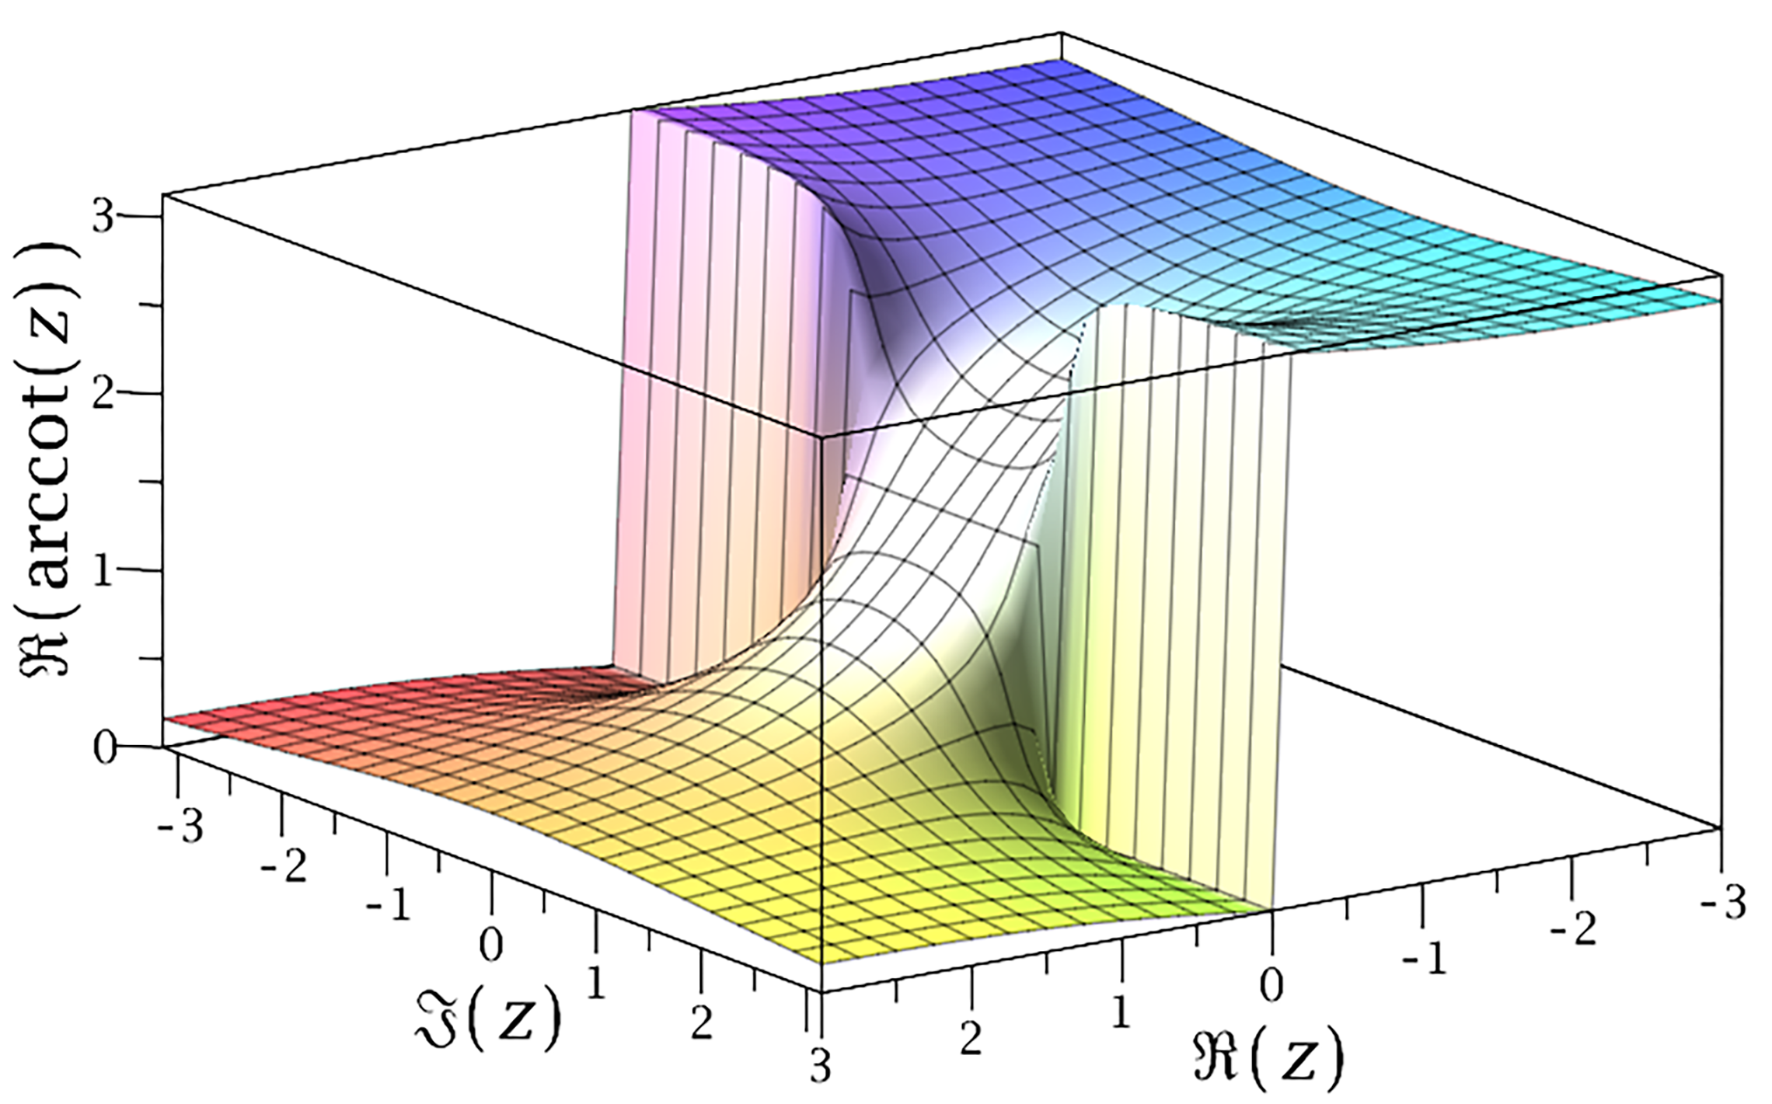
\includegraphics[width=0.45\textwidth]{acotCut1.png}
        \label{fig:acot-cut1}%
    }
    \hspace{0.5cm}
    \subfloat[The real part of arccotangent with a branch cut at ${[-\iunit, \iunit]}$.]{%
        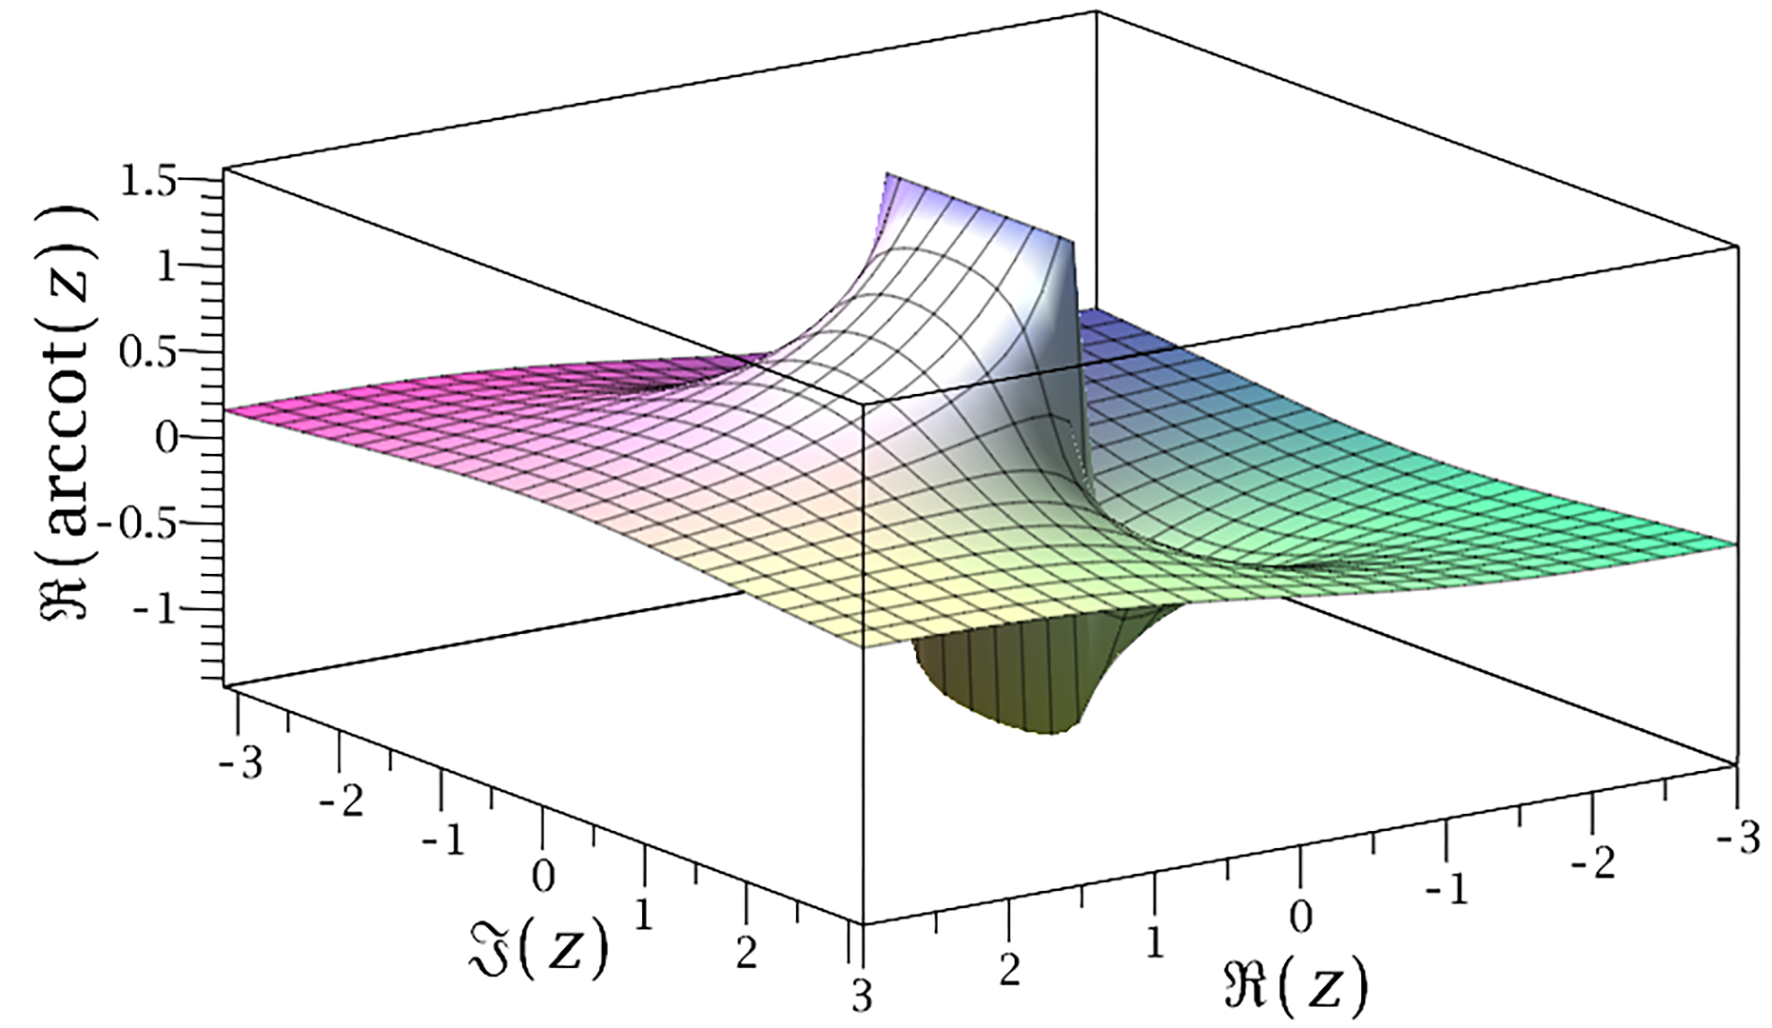
\includegraphics[width=0.45\textwidth]{acotCut2.png}
        \label{fig:acot-cut2}%
    }
    \caption{Two plots for the real part of the arccotangent function with a branch cut at $[-\iunit\infty, -\iunit]$, $[\iunit,\iunit\infty]$ in Figure~\protect\subref{fig:acot-cut1} and at $[-\iunit, \iunit]$ in Figure~\protect\subref{fig:acot-cut2}, respectively. (Plotted with \Maple{} 2016)}
    \label{fig:acot-cut-compare}
\end{figure}

Hence, a \gls*{cas} user needs to fully understand the properties and special definitions (such as the position of branch cuts) in the \gls*{cas} to avoid mistakes during a translation~\parencite{Maple:Cuts}. In consequence, a manual translation process is not only laborious, but also prone to errors. Note that this general problem has been named to automatic \gls*{p2c} conversion~\parencite{POM-Tagger}.

This article presents a new approach for automatic \gls*{p2c} and vice versa conversions. Translations from presentational to computational (computational to presentational) systems are called forward (backward) translations. A forward translation is denoted with an arrow with the target system language above the arrow. For example,
\begin{equation*}
t \overset{\langMaple}{\mapsto} c,
\end{equation*}
where $t$ is an expression in the \LaTeX{} language and $c$ is an element of the \Maple{} language $\langMaple$. As we will see later in this article, we need to compare mathematical concepts between systems. This is impossible from a mathematical point of view. Consider the irrational mathematical constant $e$, known as Euler's number. The theoretical construct for this symbol cannot be mathematically equivalent to the value \verb|exp(0)| in \Maple, caused by computational and implementational limitations. Instead of using the term \textit{equivalent}, we introduce a \textit{appropriate} and \textit{inappropriate} translations. We call a translation such as
\begin{equation}\label{eq:cos-def}
\verb|\cos@{z}| \overset{\langMaple}{\mapsto} \verb|cos(z)|
\end{equation}
as \textit{appropriate}, while a translation such as
\begin{equation}
\verb|\cos@{z}| \overset{\langMaple}{\mapsto} \verb|sin(z)|
\end{equation}
as \textit{inappropriate}. Note that it is not always as easy as in this example to decide if a translation is appropriate or not. Therefore, this article also presents several validation techniques to automatically verify if a translation is appropriate or inappropriate. In addition to this terminology, we introduce \textit{direct translations}. Later in the paper, we will explain that a translation from one specific mathematical object to its \textit{appropriate} counterpart in the other system is not always possible. We call a translation to the \textit{appropriate} counterpart \textit{direct}. For example, the translation~(\ref{eq:cos-def}) is \textit{direct}, while a translation to the definition of the cosine function
\begin{equation*}
\verb|\cos@{z}| \overset{\langMaple}{\mapsto} \verb|(exp(I*z)+exp(-I*z))/2|
\end{equation*}
is not a \textit{direct} translation.

Note that partial results of this paper have been published in~\parencite{CICM:Paper}.


%\section{Background \& Related Work}\label{ch:background}
%Before we start to explain the translation process, we need to introduce some basic information. We will see that it is not as easy as it seems to explain what semantic information is, that there can be hidden complexity even behind simple mathematical expressions, and why we need grammar to understand mathematics. All this requires a comprehensive introduction.

In this chapter we will lay the foundation to understand the complexity and our solutions in this project. The first section~\ref{sec:related-work} talks about the ideas and problems of related work. In the following section~\ref{sec:math-background}, we will give an introduction to complex analysis, branch cuts and special functions in general. Sections~\ref{sec:dlmf} and \ref{sec:semantics} will introduce the \gls{dlmf} and semantic \LaTeX, which is the most important part for our translations to \gls{cas}. Section~\ref{sec:cas} will give a brief introduction to \gls{cas} and mainly discusses \Maple{} and \Mathematica. The \gls{mlp} is another important part of the translation process, because it gives us the opportunity to parse mathematical expressions. Section~\ref{sec:mlp} explains how this works and why this is so important for a translator. This chapter finishes then with some extra definitions for the rest of the thesis.

Later on we will focus on the translation process between mathematical expressions in semantic \LaTeX{} and in \gls{cas}, where the source of semantic \LaTeX{} is the \gls{dlmf} and the source for \gls{cas} expressions is the corresponding \gls{cas}. Because there is no umbrella term for those representations from different sources, we hereafter call them \textit{systems}. A translation between semantic \LaTeX{} and \Maple{} is therefore in general a translation between two different systems.
%\section{Related Work}\label{sec:related-work}
Since \LaTeX{} became the de facto standard for writing papers in mathematics, most of the \gls*{cas} provide simple functions to import and export mathematical \LaTeX{} expressions%
\footnote{The selected \gls*{cas} Maple, Mathematica, Matlab, and SageMath provide import and/or export functions for \LaTeX:\\
Maple, \url{http://www.maplesoft.com/support/help/Maple/view.aspx?path=latex} seen 06/2017;\\
Mathematica, \url{https://reference.wolfram.com/language/tutorial/GeneratingAndImportingTeX.html} seen 06/2017;\\
Matlab, \url{https://www.mathworks.com/help/symbolic/latex.html} seen 06/2017;\\
SageMath, \url{http://doc.sagemath.org/html/en/tutorial/latex.html} seen 06/2017}. %
Those tools have two essential problems. They are only able to import simple mathematical expressions, where the semantics are unique. For example, the internal \LaTeX{} macro \verb|\frac| always indicates a fraction. However, for more complex expressions, e.g., the Jacobi polynomial in \cref{tab:JacobiP-usecase}, the import functions fail. The second problem appears in the export tools. Mathematical expressions in \gls*{cas} are fully semantic, otherwise the \gls*{cas} wouldn't be able to compute or evaluate the expressions. During the export process, the semantic information gets lost, because generic \LaTeX{} is not able to carry semantic information. In consequence of these two problems, an exported expression cannot be imported to the same system again in most cases (except those simple expressions described above). Our tool should solve these problems and provide round trip translations between \LaTeX{} and \gls*{cas}.

The semantics must be well known before an expression can be translated. There are two naiv approaches to solve that problem: (1) someone could specify the semantic information during the writing process (pre-defined semantics) or (2) the translator can find out the right semantic information in general mathematical expressions before it translates the expression. So called \textit{interactive documents}\footnote{There is no adequate definition what interactive documents are. However, this name is widely used to describe electronic document formats that allow interactivity to change the content in real time.}, such as the \gls*{cdf}~\parencite{CDF:Wolfram} by Wolfram Research or the \textit{worksheets} by \Maple{}, try to solve this problem with approach (2) and allow to embed semantic information into the input. Those complex document formats require specialized tools to show and work with the documents (Wolfram CDF Player, or \Maple{} for the \textit{worksheets}). The \JOBAD{} architecture~\parencite{JOBAD:orig} is able to create web based interactive documents and uses \gls*{omdoc}~\parencite{OMDoc} to carry semantics. The documents can be viewed and edited in the browser. Those \JOBAD{-documents} also allow to perform computations during \gls*{cas}. This gives the opportunity to calculate, compute and change mathematical expressions directly in the document. The translation performs in the background, invisible for the user. Similar to the \JOBAD{} architecture other interactive web documents exist, such as \textit{MathDox}~\parencite{MathDox} and \textit{The Planetary System}~\parencite{Planetary}. All of them demonstrate the potential for the education system.

%All of these systems carry semantic information. Most of them create their own way to make this possible. The web based documents mostly use standardized ways, such as the content \gls*{mathML}, a specialization of \gls*{mathML}~\parencite{MathML}, that focuses on the semantics of an expression rather than any particular rendering for the expression. Since \LaTeX{} is the de facto standard to write mathematical expressions in documents there are projects to extend \LaTeX{} in a way that enable to carry the semantic information directly in \LaTeX. There are two known projects that created a semantic version of \LaTeX: \sTeX{}~\parencite{sTeX} developed by Michael Kohlhase and the \Macro s developed by Bruce Miller. Our translator uses the \Macro s rather than \sTeX. A full explanation of this decision will be given in \cref{sec:semantics}.

%However, \textit{interactive documents}, web based or not, have an essential problem: all of them create an entire new document format. We want to create an independent lite translation tool for \LaTeX. Once we achieve this goal, an integration into \textit{interactive documents} might be possible, besides many other possible applications.

Another approach tries to avoid translation problems by allow computations directly via the \LaTeX{} compiler, e.g., \textit{LaTeXCalc}~\parencite{LatexCalc}. Those packages are limited to the possibilities of the compiler and therefore not as powerful as \gls*{cas}. A workaround for this case is \textit{sagetex}~\parencite{Sagetex}, which is a \LaTeX{} package interface for the open source \gls*{cas} \textit{sage}\footnote{An abbreviation for \textit{SageMath}.}. This package allows \textit{sage} commands in \TeX{-}files and uses \textit{sage} in the background to compute the commands. In this scenario, a writer still needs to manually translate expressions to the syntax of \textit{sage}.

%Obviously, the first example is not as powerful as a \gls*{cas} would be. However, \textit{sagetex} does not really solve our problem of the scientific workflow. The writer still needs to translate expressions manually. The only difference is that the author can write computations directly into the \TeX -file. However, these approaches have the potential for a powerful combination with our translation tool.

%In summary, today's translation tools are either specialized for one specific \gls*{cas} (such as the import and export functions of the \gls*{cas}) or they completely avoid the translation process by creating a new document format (such as \textit{interactive documents}). Our goal is to provide a lite translation tool for mathematical \LaTeX{} expressions and multiple \gls*{cas}.

There exists two approaches that allow to embed semantic information within \LaTeX{} expressions by using custom macros. Namely, \sTeX{}~\parencite{sTeX} developed by Kohlhase and the \Macro s developed by Miller~\parencite{DLMF:Macros}. This paper shows that it is possible to develop a context-free translation tool using the semantic macros introduced by these two projects. \sTeX{} aims to embed semantic information for general mathematics with a comprehensive set of macros. The macro set developed by Miller introduces new macros for special functions, orthogonal polynomials, and mathematical constants. Each of these macros ties specific character sequences to a well-defined mathematical object and is linked with the corresponding definition in the \gls*{dlmf} or \gls*{drmf}. Therefore, we call these semantic macros \Macro s. These semantic macros are internally used in the \gls*{dlmf} and the \gls*{drmf}. Because of the linked definitions to the \gls*{dlmf} and the special macros for functions and mathematical constants this paper using the \Macro s for performing translations to \gls*{cas} instead of using \sTeX.
%%\section{Mathematical Background}\label{sec:math-background}
%To understand the following chapters in the thesis, we need a brief introduction in complex analysis and multivalued functions. The following mathematical introduction is based on the book \textit{Introduction to Complex Analysis} by H.~A.~Priestley~\parencite{ComplexAna:Intro}.

%A complex number $z \in \Complex$ is specified by a two real numbers $x$ and $y$ as $z = x+y\iunit$, with $\iunit$ as the imaginary unit, which is defined as a solution of $\iunit^2 = -1$. The two real numbers are called the real part $x = \Re(z)$ and the imaginary part $y = \Im(z)$ of $z$. It is convenient to represent complex numbers as points in a $\Real^2$ plane, which is called \textbf{complex plane}. We identify $z = x+y\iunit$ as $(x,y) \in \Real^2$ in the complex plane. It is sometimes useful to represent complex numbers by polar coordinates and write $x = r\cos@@{\phi}$ and $y = r\sin@@{\phi}$, with $r \geq 0$ and $\phi \in \Real$. Since $\cos@@{\phi}+\sin@@{\phi}\iunit$ can be written as $\expe^{\iunit\phi}$, we write $z = x+y\iunit$ in polar coordinates as $z = r\expe^{\iunit\phi}$. The angle $\phi$ is often called the \textbf{phase} (or argument) of $z$ and $r$ is the absolute value of $z$. Similar to $\Re(z)$ for the real part and $\Im(z)$ for the imaginary part of $z$, we can access $r = |z|$ and $\phi = \ph@{z}$.\footnote{Note that the phase of $z$ is often called the \textbf{argument} of $z$. Therefore, in CAS the phase function is often the \texttt{argument} function.}

%\begin{figure}[ht]
%    \centering
%    \subfloat[Four color phase mapping.]{%
%        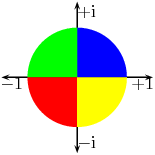
\includegraphics[width=0.28\textwidth]{dlmfColorMap.png}
%        \label{fig:four-color}%
%    }
%    \hspace{0.4cm}
%    \subfloat[Continues phase mapping in \DLMF.]{%
%        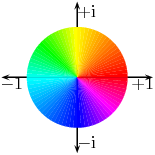
\includegraphics[width=0.28\textwidth]{dlmfColorMapCont.png}
%        \label{fig:cont-color}%
%    }
%    \hspace{0.4cm}
%    \subfloat[Continues phase mapping in \Maple.]{%
%        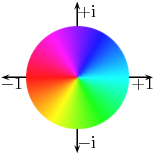
\includegraphics[width=0.28\textwidth]{mapleColorMap.png}
%        \label{fig:maple-color}%
%    }
%    \caption{Three different domain coloring methods. Mappings~\protect\subref{fig:four-color} and \protect\subref{fig:cont-color} used in the \DLMF{} (Source: \DLMF{~}\parencite{NIST:DLMF} in help page, \textit{About Color Map}). Mapping~\protect\subref{fig:maple-color} is the default coloring map in \Maple.}
%    \label{fig:domain-coloring}
%\end{figure}

%Since the same basic arithmetical rules apply in $\Complex$ as in $\Real$, we will not introduce all arithmetical rules for complex numbers here. However, another interesting part are plots of complex functions. Consider a function $f: \Complex \mapsto \Complex$. This can be considered as $f: \Real^2 \mapsto \Real^2$, which shows us four real dimensions that need to be displayed in a three-dimensional space. The most common solution to plot those four dimensions is called domain coloring. With this technique, each value in the complex plane is represented by a color. There is no standard method to map complex values to colors. A simple method is to map a unique color for each of the quadrants in the complex plane (used in the DLMF). Another variation are continues phase mappings, which use color wheels. In those cases, $\phi$ represents the hue and optionally $r$ defines the intensity of the hue. The second variation is mostly used in \gls{cas}, but there is no standard for the orientation of the color wheel. Figure~\ref{fig:domain-coloring} draws three different examples.

%This thesis mostly focus on the \gls{cas} \Maple, therefore all of the following complex plots use the default color map in \Maple{~}\ref{fig:maple-color}.

%A three-dimensional plot of a complex function, such as $f$ from above, usually maps the real and imaginary part of the variable to the $x$ and $y$ axes, while the height is defined by the absolute value of the complex variable $|z|$. Figure~\ref{fig:cylinderU} demonstrates a complex plot of the parabolic cylinder function $U(a,z)$~\parencite[(12.2i)]{NIST:DLMF} in \Maple. 

%\begin{figure}[ht]
%	\centering
%	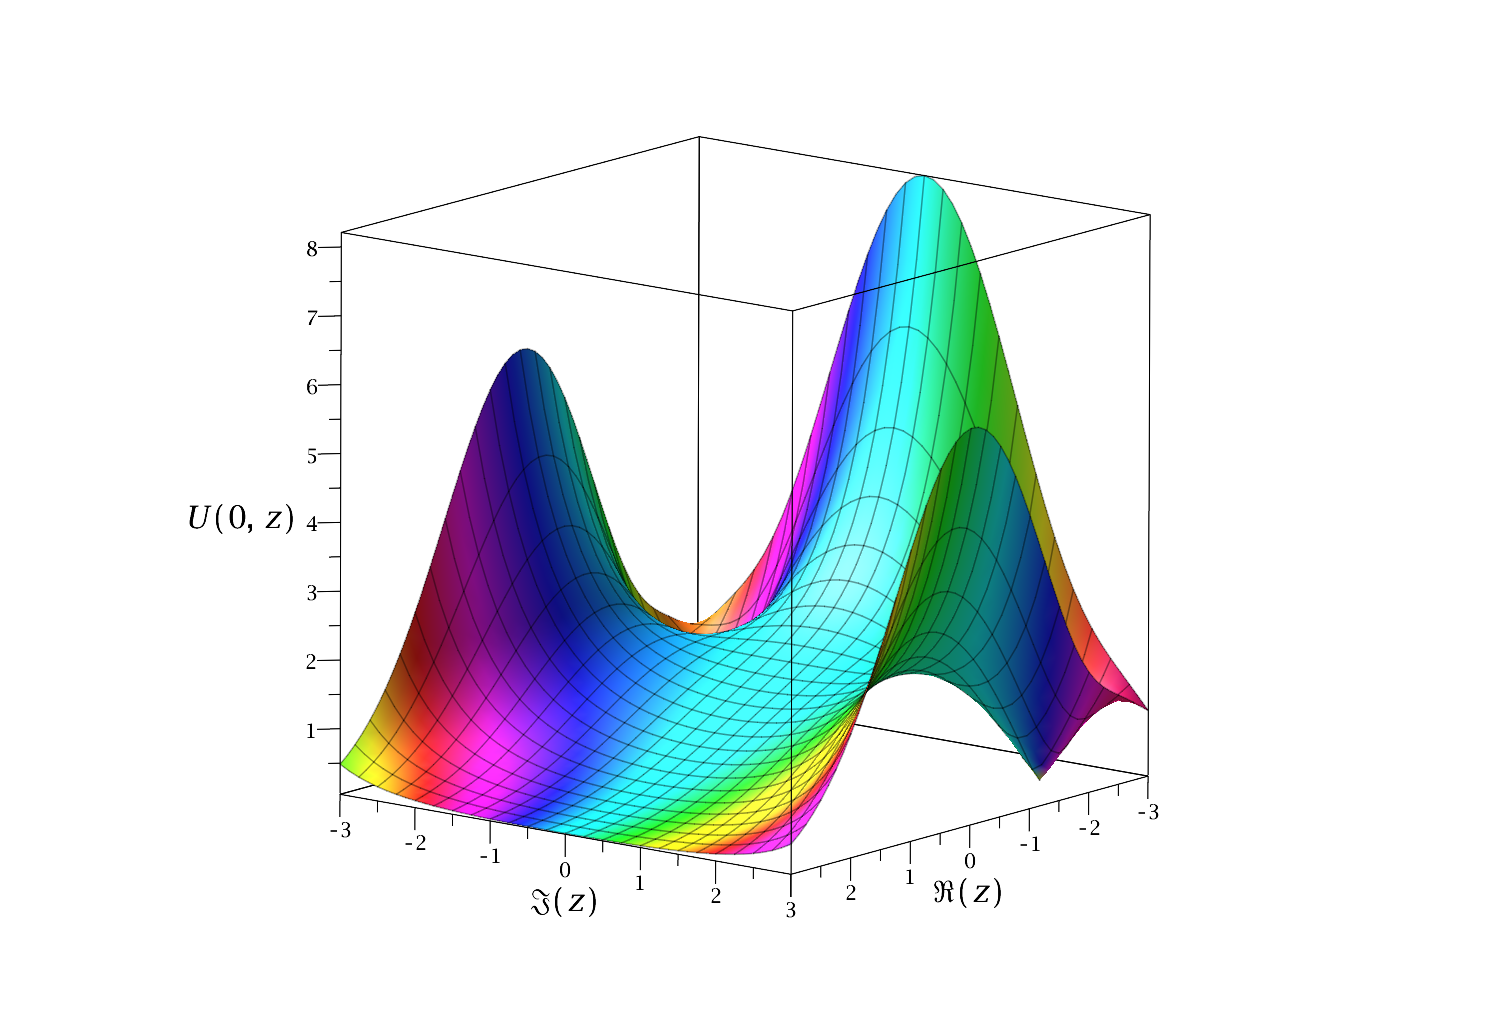
\includegraphics[width=0.8\textwidth]{cylinderUPlot.png}
%	\caption{A 3-dimensional complex plot of the parabolic cylinder function $U(a,z)$ at $a=0$ plotted by \Maple.~\parencite[(12.2i)]{NIST:DLMF}}
%	\label{fig:cylinderU}
%\end{figure}

%Another way to plot such complex functions is to plot the real and imaginary parts of the solution separately. Figure~\ref{fig:cylinderUSplit} illustrates this plotting method for the parabolic cylinder function again. 

%Note that for real function plots, such separate plots for the imaginary and real values of a complex function, will use a color map as well. In that case, the color map is just an adornment and has nothing to do with complex color maps. Figure~\ref{fig:cylinderUSplit} illustrates the separate plots for real and imaginary values for the parabolic cylinder function again.

%\begin{figure}[!htp]
%    \centering
%    \subfloat[Plot of the real value of $\ParabolicU@{0}{z}$.]{%
%        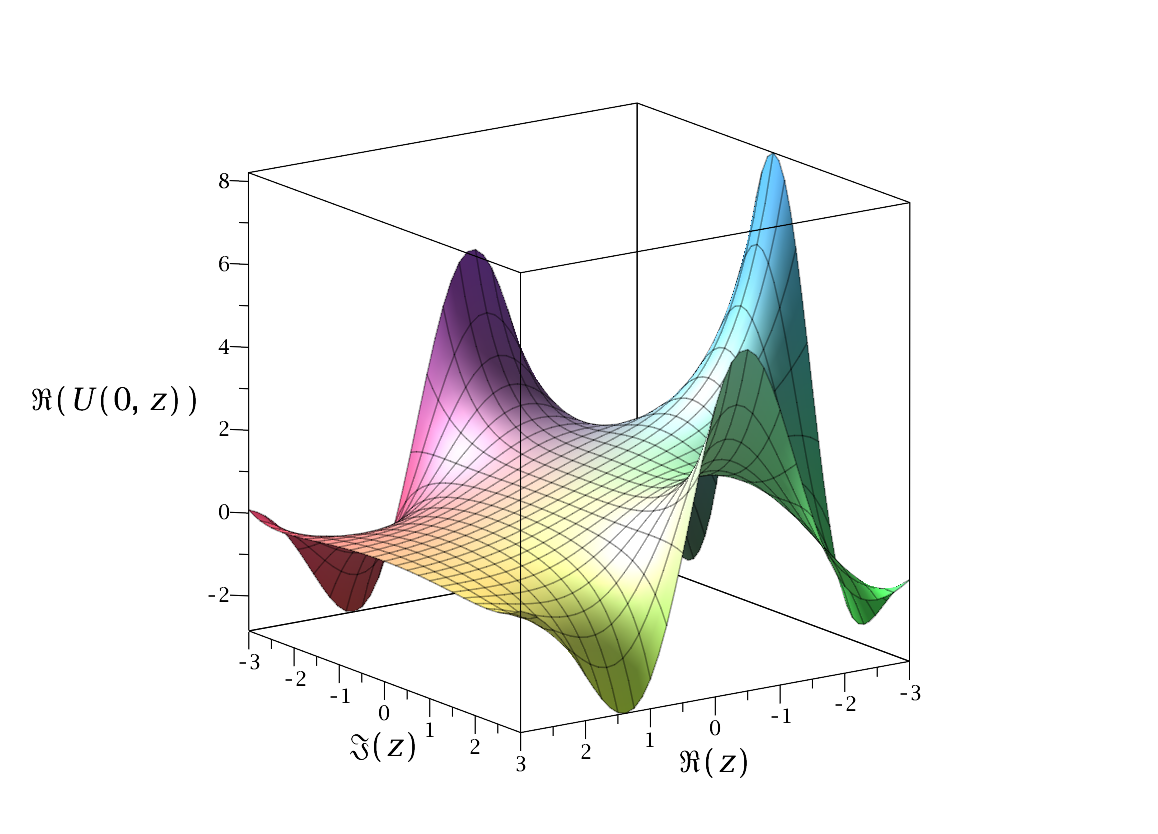
\includegraphics[width=0.8\textwidth]{cylinderURe.png}
%        \label{fig:cylinderURe}%
%    }
%    \vspace{-0.1cm}
%    \subfloat[Plot of the imaginary value of $\ParabolicU@{0}{z}$.]{%
%        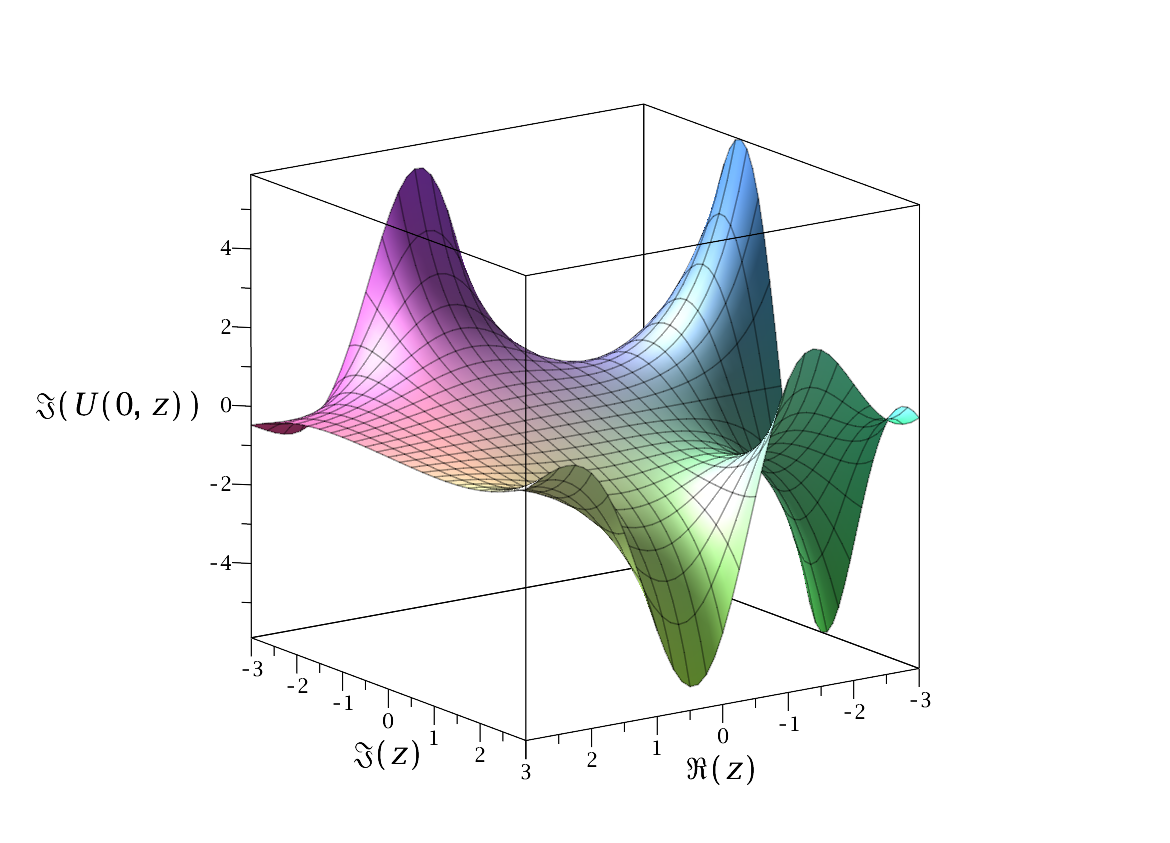
\includegraphics[width=0.8\textwidth]{cylinderUIm.png}
%        \label{fig:cylinderUIm}%
%    }
%    \caption{Separately plot of the real~\protect\subref{fig:cylinderURe} and imaginary~\protect\subref{fig:cylinderUIm} part of the parabolic cylinder function $U(a,z)$ at $a=0$.}
%    \label{fig:cylinderUSplit}
%\end{figure}

%\subsection{Multivalued Functions}
%The following definitions for multivalued functions are based on \textit{Complex Variables}~\parencite{ComplexVariables} by M.~J.~Ablowitz and A.~S.~Fokas.

%Unlike a typical\footnote{In lack of a better word to distinguish single-valued and multivalued functions, we call single-valued functions here typical functions, because these functions are best known.} function, multivalued functions associate not only one output to any particular input, but a whole set of output values. A real-valued example is the square root function, which associates for each positive real number two real square roots. For example\footnote{Note that the radical sign $\sqrt{}$\ is defined for the principal square roots, which are the unique non-negative square roots. Therefore, $\sqrt{4}$ is always $2$, and not $-2$. However, the solutions of the square root of a positive number $a$ are $\left\{+\sqrt{a},-\sqrt{a}\right\}$.}, the solution of $4^{\frac{1}{2}}$ is $\{+2,-2\}$.

%Consider now the natural logarithm with complex arguments and $z = r\expe^{\iunit\phi}$ in polar coordinates. Since it is the natural logarithm, $\ln@{z} = \ln@{r} + \iunit\phi$ and the imaginary part is just $\phi$. Let $r = 1$, so that $z$ is on the unit circle for all $\phi$. Let be $z_1$ the complex number for $\phi = 0$ and $z_2$ the complex number for $\phi = 2\cpi$. Obviously $z_1 = z_2$ but $\ln@{z_1} \neq \ln@{z_2}$. Therefore, the natural logarithm is also multivalued and has an infinite number of solutions for $\ln@{z}$. 

The center of the circle we choose (in that case the origin) is called branch point.

\begin{definition}[Branch Point]
A point $p$ is a \textbf{branch point} if the multivalued function $w(z)$ is discontinuous upon traversing an arbitrarily small circuit around $p$.
\end{definition}

The complex square root function has also a branch point in the origin. Consider
\begin{equation}
\sqrt{z} = \sqrt{r} \expe^{\frac{\iunit\phi}{2}},\quad \text{with } r \geq 0, \phi \in \Real.
\end{equation}
Indeed, at $\phi = 2\cpi$, the square root of $z$ is $\sqrt{r}\expe^{\iunit\cpi} = -\sqrt{r}$, but at $\phi = 0$ it is $\sqrt{r}$. Because $r$ was arbitrary, the origin is also a branch point of the complex square root function. Another branch point is $z = \infty$.

There exist two approaches to analytically study multivalued functions. One approach is to express the multivalued function as a single-valued function.

\subsubsection{Branch Cuts}\label{subsec:branch-cuts}
Consider a multivalued function in a restricted region and choose for every argument a value, such that the resulting function in the region is continues and single-valued. This regional function of the multivalued function is called \textbf{branch} of the multivalued function. 

Consider the complex square root function again. If we cut out the region between both branch points, namely $(0, \infty)$, the function is continues and single-valued. This region is one branch of the function and the cut region $(0, \infty)$ is called \textbf{branch cut}. Another branch of the function can be reached by further increasing $\phi$, such that $\phi \in [2\cpi, 4\cpi)$. At $\phi = 4\cpi$ the square root function returns the same result as for $\phi=0$. Therefore, $\phi \in [4\cpi, 6\cpi)$ is again on the first branch. We can define a branch cut for the complex logarithm as well. As already mentioned, the complex logarithm has an infinite number of branches. Each of these branches can be reached by increasing or decreasing $\phi$ with a multiple of $2\cpi$. Consider $\phi+n2\cpi$ with an integer number $n$. The branch for $n=0$ is called the \textbf{principal branch}.

Defining branch cuts to allow analytic computations on the principal branches is a common task for \gls{cas}~\parencite{Maple:Cuts}. Unfortunately, the position of the branch cuts is not well-defined. Indeed, consider $\phi \in [-\cpi,\cpi)$ instead of $\phi \in [0,2\cpi)$ and define the branch cut at $(-\infty, 0)$; than the branch is also continues and single-valued. 

In general a branch cut is a curve which ends can be possibly open, half-open or closed. A branch cut can be also defined in a more complicated shape (e.g. spirals). Most of the multivalued functions have standard, convenient positions for the branch cuts, which are commonly accepted. The branch cut at $(-\infty, 0]$ for the complex square root function is one of those standard positions. However, the positions can vary from system to system~\parencite{Branches:acot}.

Figure~\ref{fig:sqrtBranch} draws the principal branch of the imaginary part of the complex square root function in \Maple.
 
\begin{figure}[ht]
	\centering
	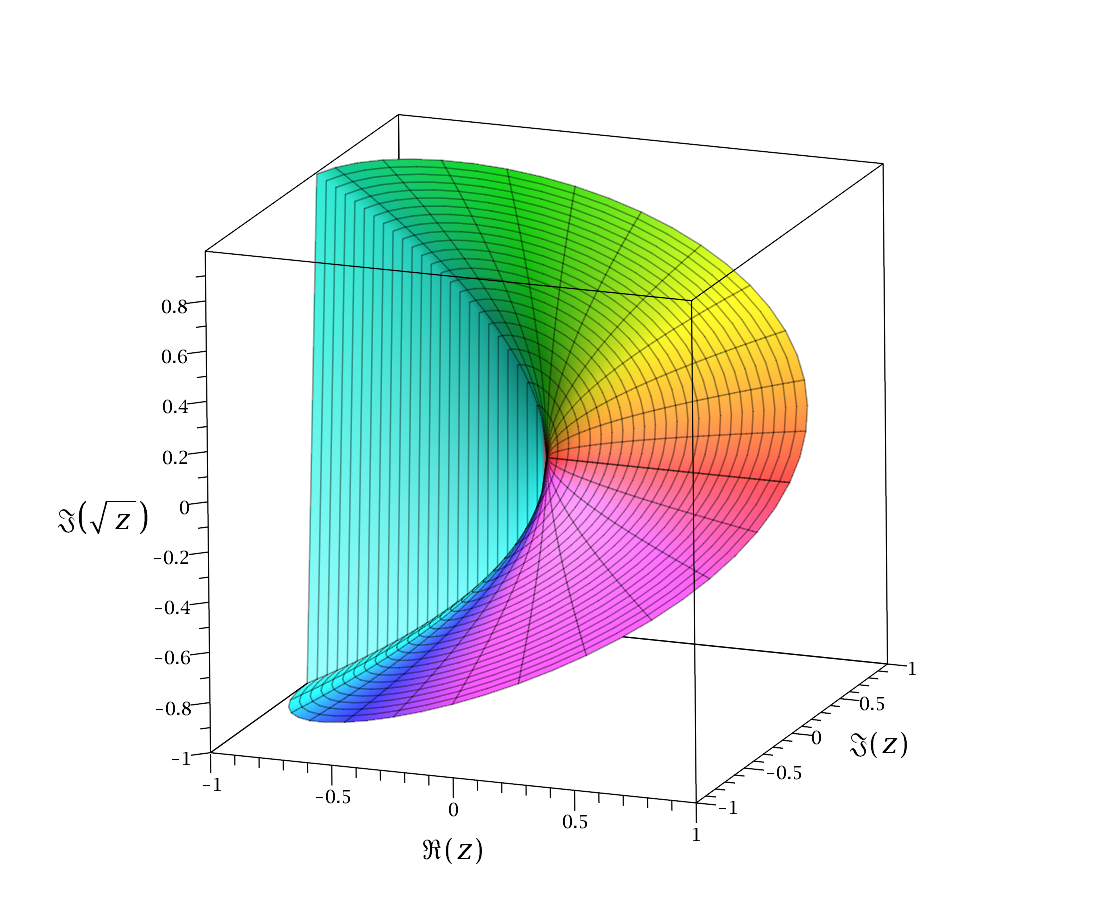
\includegraphics[width=0.65\textwidth]{sqrtBranch.png}
	\caption{The imaginary part of the complex square root function with a branch cut at $(-\infty, 0)$. The resulted function is continues and single-valued for $\phi \in (-\cpi, \cpi)$.}
	\label{fig:sqrtBranch}
\end{figure}

The plot of the principal branch for the complex logarithm looks similar. The branch cut for the logarithm is in \Maple{} defined at $(-\infty,0)$. Figure~\ref{fig:lnBranch} illustrates the principal branch of the imaginary part of the logarithm.

\begin{figure}[H]
	\centering
	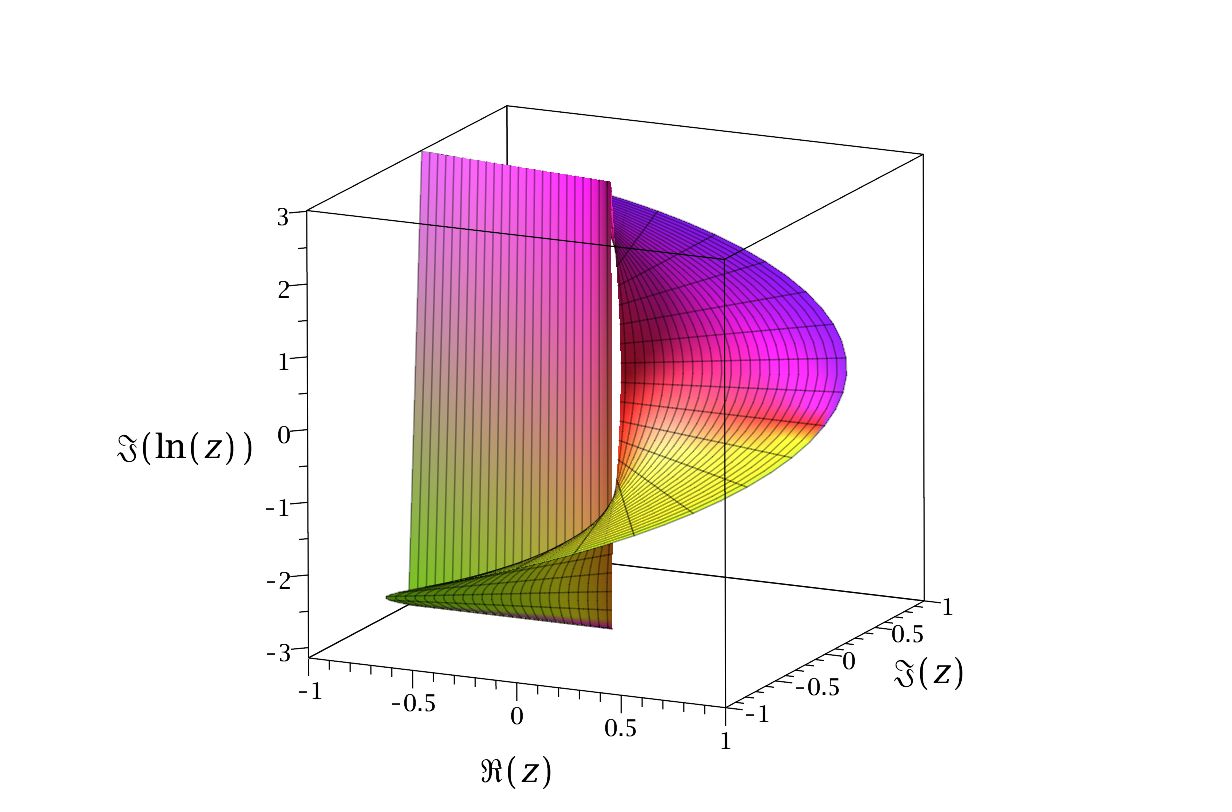
\includegraphics[width=0.75\textwidth]{lnBranch.png}
	\caption{The imaginary part of the complex logarithm with a branch cut at $(-\infty, 0]$. The resulted function is continues and single-valued for $\phi \in (-\cpi, \cpi)$.}
	\label{fig:lnBranch}
\end{figure}

Note that in complex plots, a branch cut can also be located in the color map, we were talking about above. In the next example, we use the notation $\pm 0$ to come arbitrarily close to the branch cut from the \textit{upper} and \textit{lower} side. We presume the one-side limits is a well known notation and define
\begin{align}
-0 &:= \underset{x\nearrow 0}{\lim}x,\\
+0 &:= \underset{x\searrow 0}{\lim}x.
\end{align}

The natural logarithm $\ln@{z}$ has a branch cut at $(-\infty,0]$. We have the following values for the \textit{upper side} and \textit{lower side} of the branch cut at $\ln@{-1}$
\begin{align}
\ln@{-1+\iunit 0} &=\hphantom{-}\iunit \cpi,\label{eq:ln-up}\\
\ln@{-1-\iunit 0} &= -\iunit \cpi.\label{eq:ln-down}
\end{align}

Figure~\ref{fig:ln-compl-comp} shows two plots of the natural logarithm. The value of (\ref{eq:ln-up}) is represented by a shade of purple and (\ref{eq:ln-down}) is represented by a shade of green, with \Maple's continues phase color map from figure~\ref{fig:maple-color}. The branch cut can be seen by the changing of the color from purple directly to green on $(-\infty,0]$. The colors are counterparts of each other in the used color map.

\begin{figure}[!htp]
    \centering
    \subfloat[The complex plot for the natural logarithm $\ln@{z}$. The values of $\ln@{z}$ are visualized by colors. The coloring method is the continues phase mapping from \Maple.]{%
        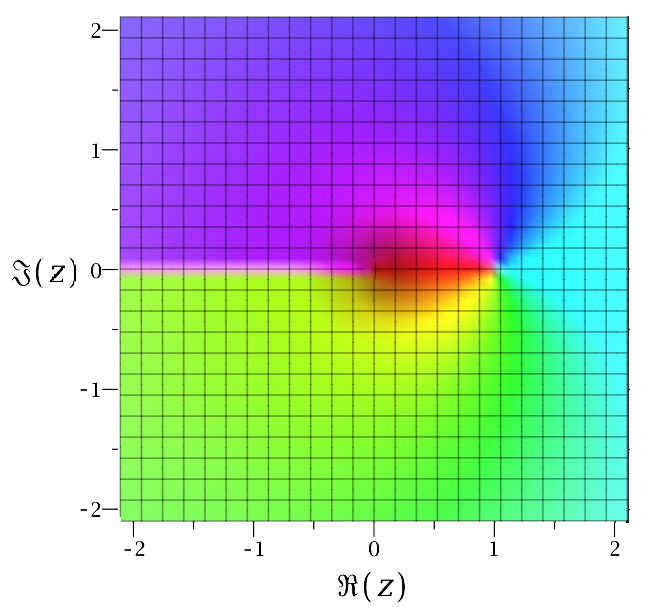
\includegraphics[width=0.4\textwidth]{lnComp1.png}
        \label{fig:ln-color}%
    }
    \hspace{0.5cm}
    \subfloat[The complex plot for the natural logarithm $\ln@{z}$. The height is the absolute value. The coloring method is the continues phase mapping from \Maple.]{%
        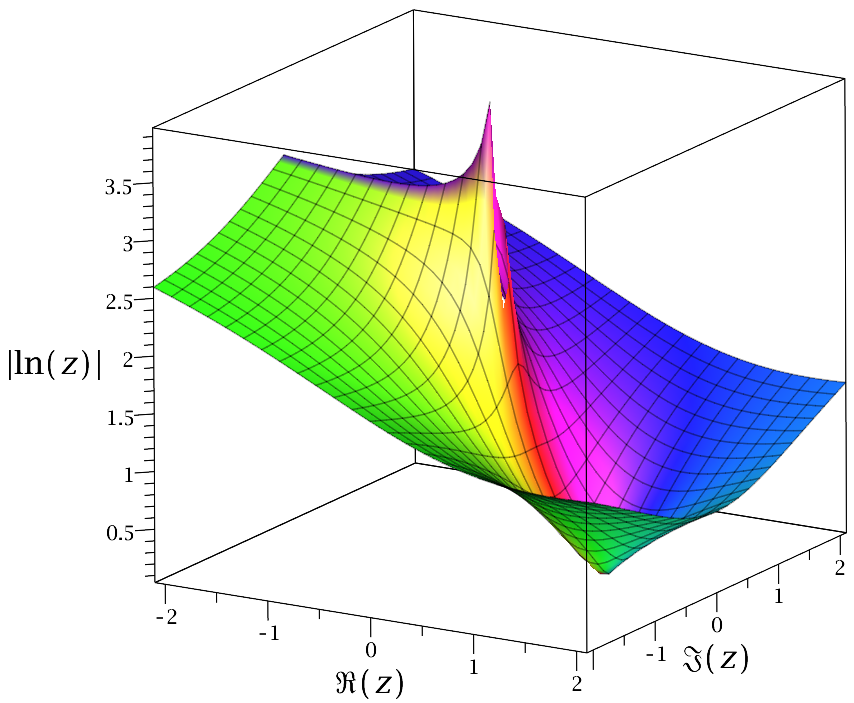
\includegraphics[width=0.47\textwidth]{lnComp2.png}
        \label{fig:ln-compl}%
    }
    \caption{The complex plot of the natural logarithm $\ln@{z}$. Figure~\protect\subref{fig:ln-color} plots only the colors of $\ln@{z}$. The coloring method is \Maple's continues phase mapping from figure~\protect\ref{fig:maple-color}. The branch cut of $\ln@{z}$ is at $(-\infty,0)$ and the values $\ln@{1+\iunit 0} = \iunit \cpi$ (which is mapped to purple), while $\ln@{1-\iunit 0} = -\iunit \cpi$ (which is represented by green).}
    \label{fig:ln-compl-comp}
\end{figure}

An alternative representation for multivalued functions to branch cuts are Riemann surfaces.

\subsubsection{Riemann Surfaces}
Assume we would not cut the multivalued functions and allow multiple values for a particular input. For example, if we allow $\phi$ to constantly increase in the complex logarithm function, we end up in helix structure as plotted in figure~\ref{fig:lnRiemann}. This representation of a multivalued function is called the Riemann surface. Technically, a Riemann surface is a one-dimensional complex manifold.

\begin{figure}[!ht]
	\centering
	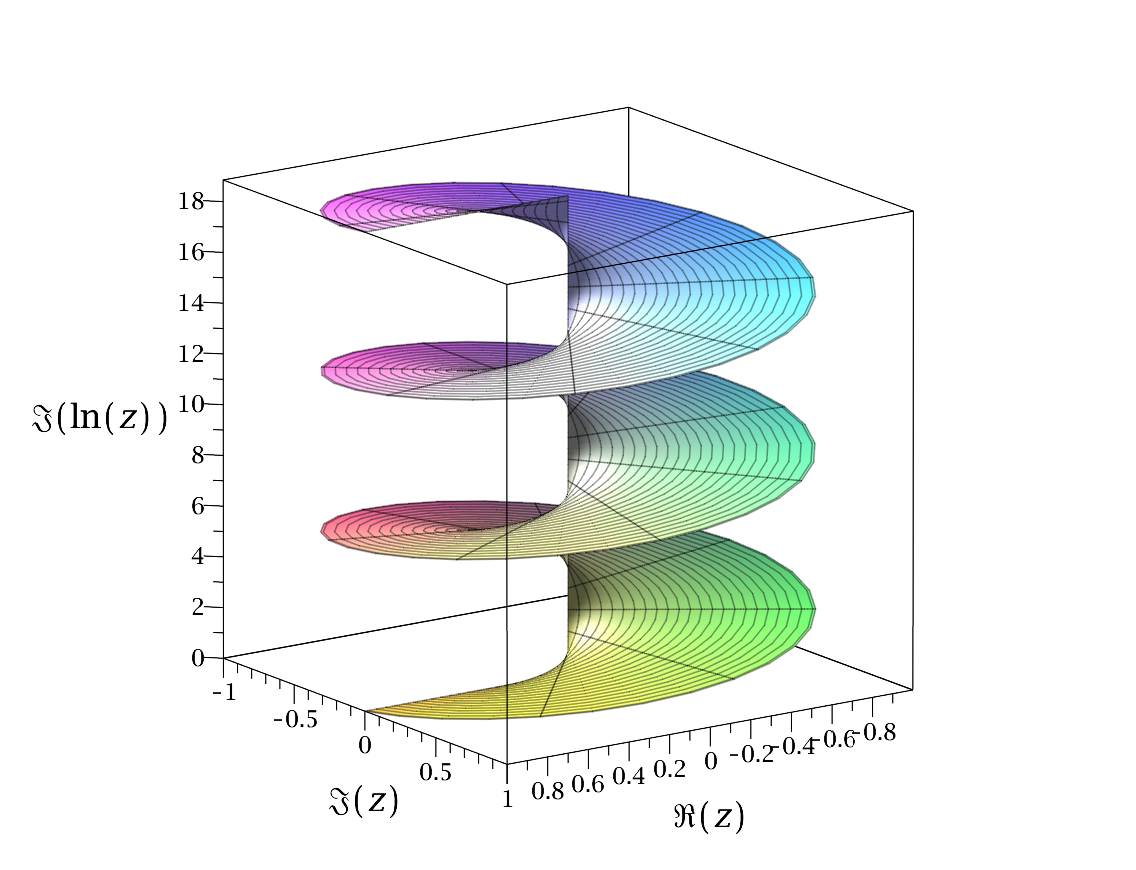
\includegraphics[width=0.8\textwidth]{lnRiemann.png}
	\caption{The Riemann surface of the imaginary part of the natural logarithm.}
	\label{fig:lnRiemann}
\end{figure}

In the Riemann surface of logarithm in figure~\ref{fig:lnRiemann} we can see the multiple branches of the function. If we use the same method for the square root function, we get figure~\ref{fig:sqrtRiemann}, where we can see that the square root function has only two branches.

\begin{figure}[!ht]
	\centering
	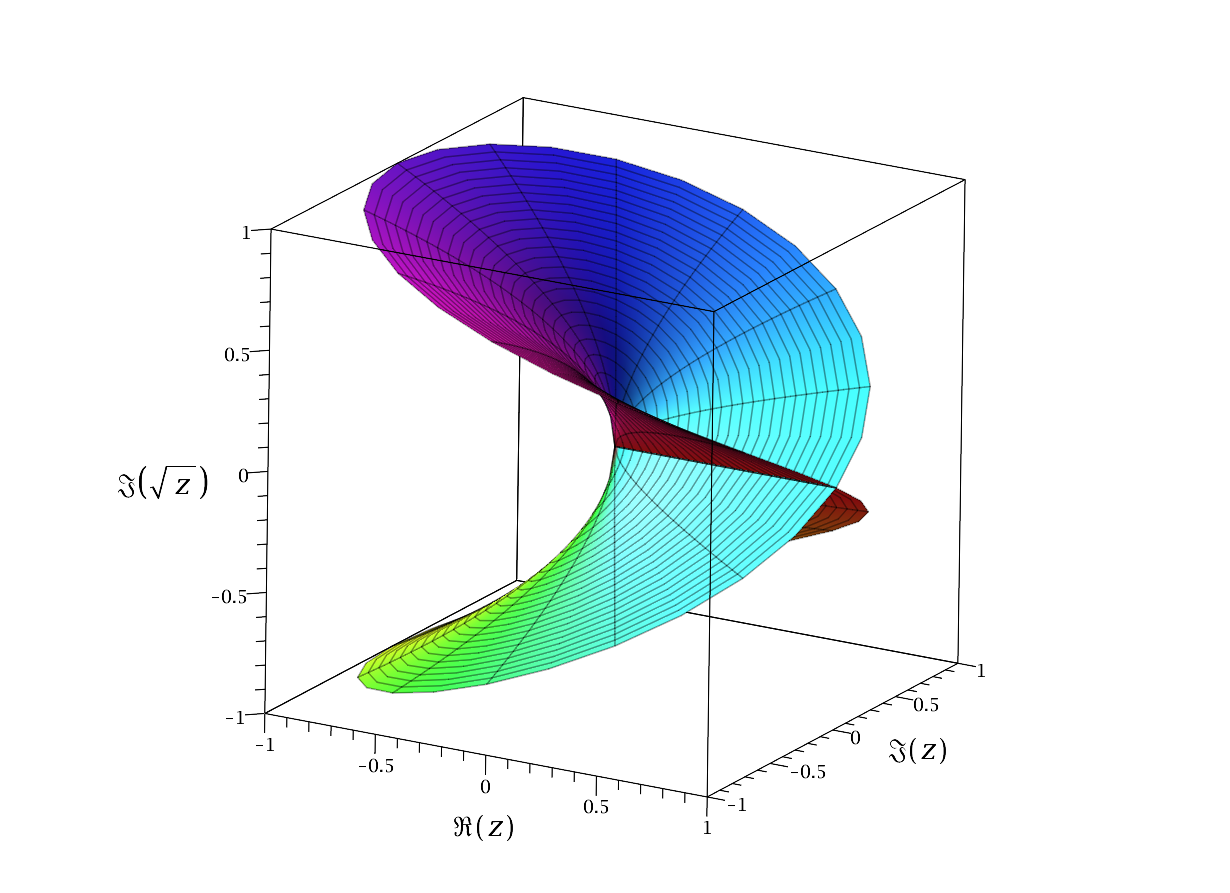
\includegraphics[width=0.9\textwidth]{sqrtRiemann.png}
	\caption{The Riemann surface of the imaginary part of the square root function.}
	\label{fig:sqrtRiemann}
\end{figure}

\subsection{Elementary \& Special Functions}\label{subsec:special-functions}
A function is called \textbf{elementary} if it can be constructed using only a finite combination of constant functions, field operations, and algebraic, trigonometric, exponential, and logarithmic functions together with their inverses~\parencites{Elementary:1}[145]{Elementary:2}.

Unlike elementary functions, special functions cannot be listed easily. They are mostly solutions of differential equations or integrals of elementary functions. Almost all of them have established names and notations. Many of them are complex and some are also multivalued. Besides that, special functions are highly related to each other. Therefore, most special functions can be expressed by other special functions. However, there is no general formal definition, but there are lists and mathematical compendia collecting functions which are commonly accepted as special. 

For example, in 1964 Milton Abramowitz and Irene A. Stegun published the \textit{Handbook of Mathematical Functions with Formulas, Graphs, and Mathematical Tables}~\parencite{AbramowitzStegun} at \gls{nist}\footnote{In 1988 the \textit{National Bureau of Standards} (NBS) was renamed to the \textit{National Instutute of Standards and Technology} (NIST).}. The handbook became the most comprehensive source of information on special functions. Therefore, the \gls{nist} has published a new version called \textit{NIST Handbook of Mathematical Function}~\parencite{NIST:Handbook} in 2010 to replace the predecessor.

Because there is no formal definition for special functions, some problems appear for our translator project. For example the \textit{Encyclop\ae{dia} Britannica} wrote:
\begin{myQuote}{Encyclop\ae{dia} Britannica - Special function~\parencite{SpecialFunctions:britannica}}
	Special function, any of a class of mathematical functions that arise in the solution of various classical problems of physics. [...] Different scientists might not completely agree on which functions are to be included among the special functions, although there would certainly be very substantial overlap.
\end{myQuote}

In \textit{Special Functions}~\parencite{SF:Book}, G.~E.~Andrews~et~al. wrote in the preface:
\begin{myQuote}{Special Functions - Preface~\parencite{SF:Book}}
Paul Tur\'an once remarked that special functions would be more appropriately labeled "useful functions".
\end{myQuote}

Our reference for special functions in this thesis will be the \textit{NIST Handbook of Mathematical Function} and its digital counterpart the \gls{dlmf}~\parencite{NIST:DLMF}. See the later section~\ref{sec:dlmf} for a more detailed explanation. 

Since most of the special functions represent solutions for other mathematical expressions, they were intensively studied - mostly in applied mathematics. In the past, huge tables of values were used for calculations~\parencite{Tables}. Therefore, the book by Abramowitz and Stegun also contains tables with values for several special functions~\parencite{AbramowitzStegun}. Obviously, computations of special functions with \gls{cas} were desired. Therefore, \gls{cas} support numerous of special functions. However, all \gls{cas} contain its own ever growing lists of them. Sometimes they use the same definitions, domains and position of branch cuts as defined the handbooks, sometimes not. A translator needs to pay attention to those differences as well. Otherwise the translation process could produce unexpected effects. One of these effects can be produced by different positions of branch cuts in the systems. The next section will give some examples and explanations of these problems.

\subsection{Problems of Branch Cuts}\label{subsec:branch-cut-issues}
Obviously, different positions of branch cuts can cause problems, if we transfer a function from one system to the other. Those differences can even appear in well-known elementary functions. For example, the \gls{dlmf} defines the branch cut for the inverse cotangent function~\parencite[(4.23.9)]{NIST:DLMF} at $[-\iunit, \iunit]$, while \Maple{} reasonably~\parencite{Branches:acot} defines the branch cut at $(-\infty\iunit, -\iunit]$ and $[\iunit, \infty\iunit)$. Figure~\ref{fig:acot} illustrates the problem. A scientist, who is familiar with the definition for the branch cut by the \gls{dlmf} would assume an output such as in figure~\ref{fig:acotCont}, but get an output such as in figure~\ref{fig:acotJump} in \Maple.

\begin{figure}[!ht]
    \centering
    \subfloat[Plot of the arccotangent function with the branch cut defined by \DLMF.]{%
        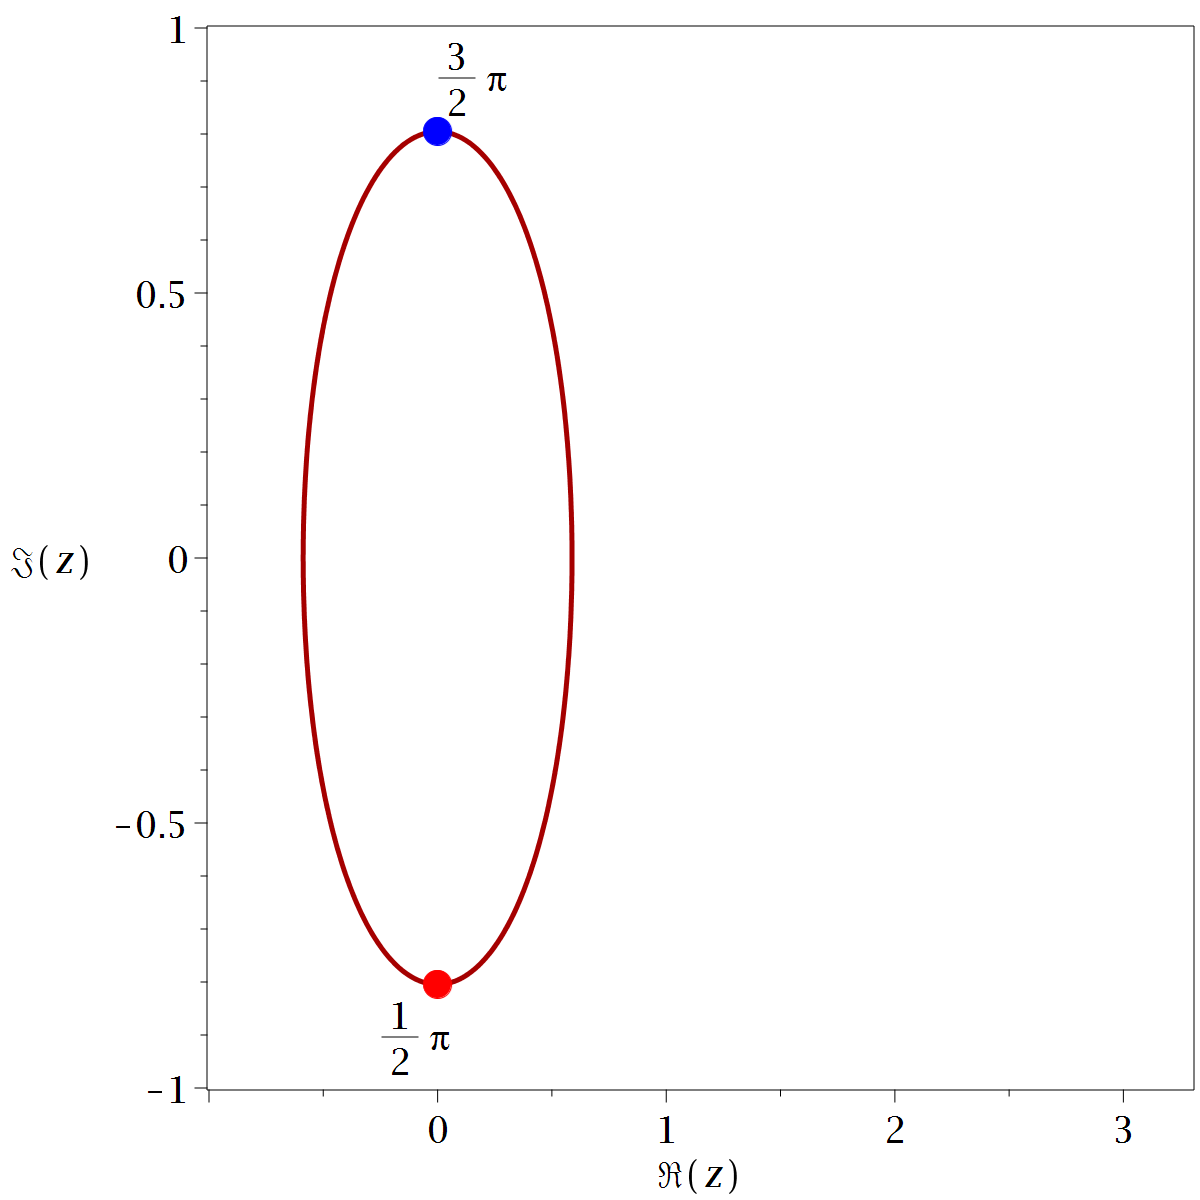
\includegraphics[width=0.45\textwidth]{acotCont.png}
        \label{fig:acotCont}%
    }
    \hspace{0.2cm}
    \subfloat[Plot of the arccotangent function with the branch cut defined by \Maple.]{%
        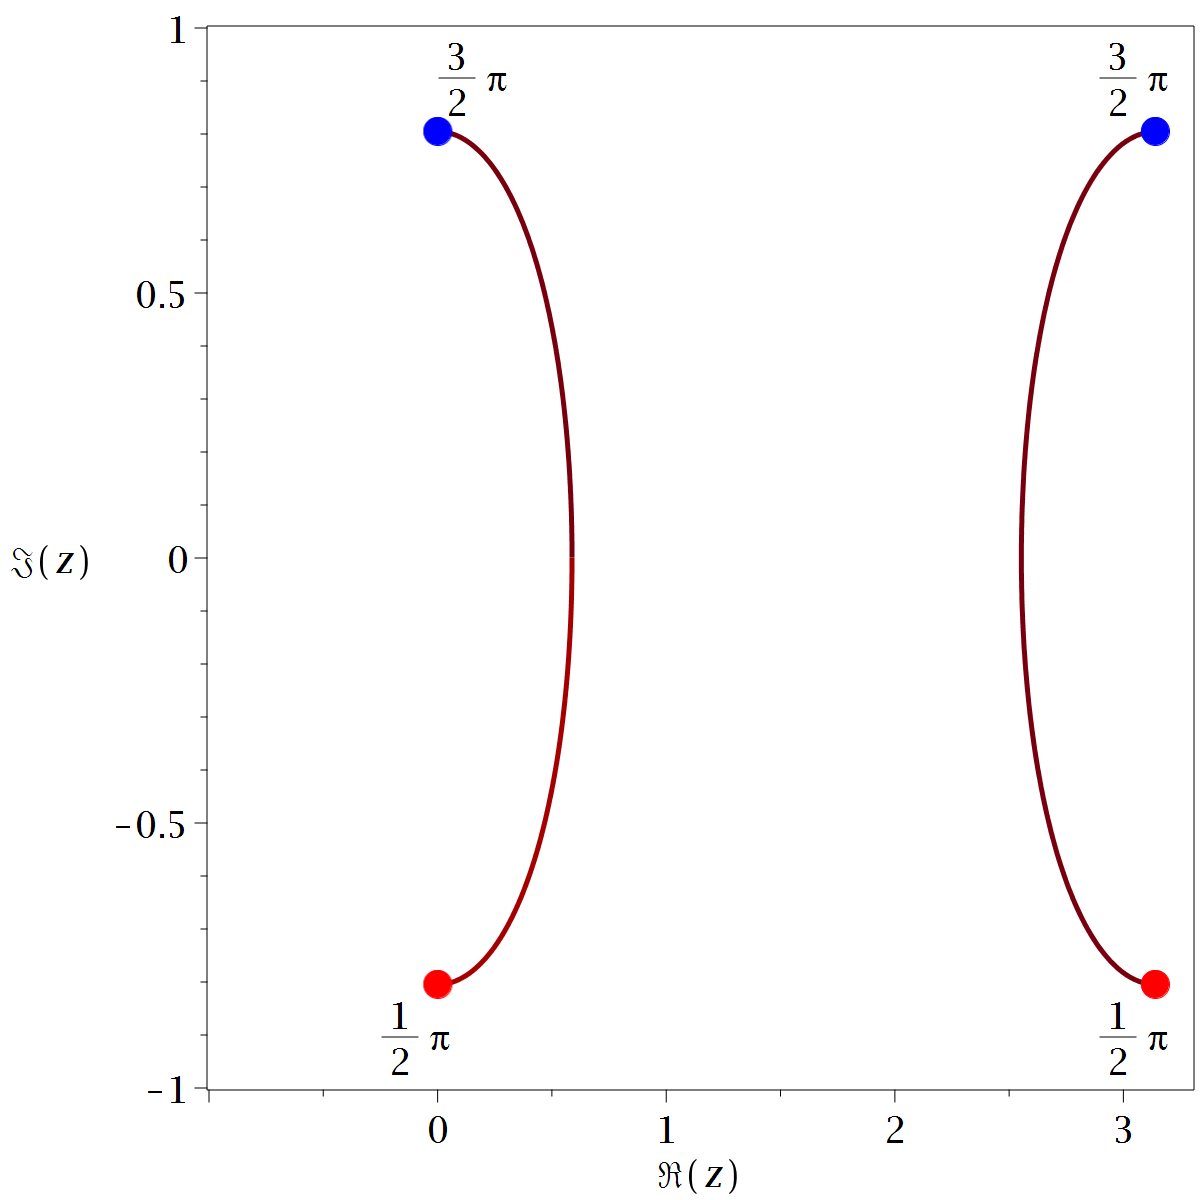
\includegraphics[width=0.45\textwidth]{acotJump.png}
        \label{fig:acotJump}%
    }
    \caption{Plots for the arccotangent function $\acot@{z}$ with $z = \frac{3}{2}\expe^{\iunit\phi}$, where $\phi \in [0,2\cpi]$. Figure~\protect\subref{fig:acotCont} illustrates a branch cut defined at $[-\iunit, \iunit]$ and figure~\protect\subref{fig:acotJump} illustrates the branch cuts defined at $(-\infty\iunit, -\iunit]$ and $[\iunit, \infty\iunit)$. The blue and red dots represents the positions, where the function jumps over the branch cuts in~\protect\subref{fig:acotJump}.}
    \label{fig:acot}
\end{figure}

We provide the following solution for such problems. Instead of translating the function itself, the translator uses other equivalent representations for the function. In case of the arccotangent function, we can use the following alternative representations, based on the suggestions in~\parencite{Branches:acot}.

Note that the following notation uses our standard notation for a translation from semantic \LaTeX{} to \Maple. We will introduce this notation in a formal way later in section~\ref{sec:definition}.

\begin{eqnarray}
\verb|\acot@{z}| & \overset{\langMaple}{\mapsto} & \verb|arccot(z)|\label{eq:acot-alternatives}\\
& \overset{\langMaple}{\mapsto} & \verb|arctan(1/z)|\label{eq:acot-alternatives-1}\\
& \overset{\langMaple}{\mapsto} & \verb|I/2*ln((z-I)/(z+I))|\label{eq:acot-alternatives-2}
\end{eqnarray}

As illustrated above, translation~(\ref{eq:acot-alternatives}) contains the branch cut issue. Translation~(\ref{eq:acot-alternatives-1}) is an alternative, because the arctangent function in \Maple{} has the same position for the branch cut of the arctangent function in the \gls{dlmf}. However, in this case, the arccotangent function would be no longer defined at $z=0$. Translation~(\ref{eq:acot-alternatives-2}) is another alternative and defined at $z=0$. 

A more complicated example might be the equation of the already introduced parabolic cylinder function $U(a,z)$ and the modified Bessel function of the second kind $\BesselK{\nu}@{z}$. The parabolic cylinder function is a solution of a second order differential equation~\parencite[(12.2i)]{NIST:DLMF} and can be represented by $\BesselK{\nu}@@{z}$ for $a=0$. The relation is defined in~(\ref{eq:branch-cut-issue}). 

\begin{equation}\label{eq:branch-cut-issue}
\displaystyle U(0,z) = \sqrt{\frac{z}{2\cpi}}\BesselK{\frac{1}{4}}@{\frac{1}{4}z^2}
\end{equation}

Following the same approach as for the arccotangent function discovers results in a branch cut problem. Figure~\ref{fig:u-bessel} illustrates that problem for equation~(\ref{eq:branch-cut-issue}) with $z=2.5\expe^{\iunit\phi}$ and letting $\phi$ increase from $0$ to $2\cpi$. While the left hand side is an entire function of $z$ (can be seen in figure~\ref{fig:u-cont}), the right hand side has two functions with a branch cut along the negative real axis each. As already discussed, the branch cut of the square root function is at $(-\infty,0]$. Therefore, at $\phi = \cpi$ the right hand side jumps over the branch cut (green dots) back to the principal branch rather than continue on the other branch. Furthermore, the principal branch of $K_\nu$ is defined for $\phi \in (-\cpi,\cpi]$. With $z^2 = r^2\expe^{2\iunit\phi}$, the branch cut of $K_\nu$ is reached at $\phi = \left\{ \frac{\cpi}{2}, \frac{3\cpi}{2} \right\}$ (red dots and blue dots). The branch cut of $K_\nu$ "moves" to $(-\infty\iunit,0]$ and $[0,\infty\iunit)$. Hence, we end up with three branch cuts for the right hand side of (\ref{eq:branch-cut-issue}).

\begin{figure}[!ht]
    \centering
    \subfloat[The left hand side of (\ref{eq:branch-cut-issue}).]{%
        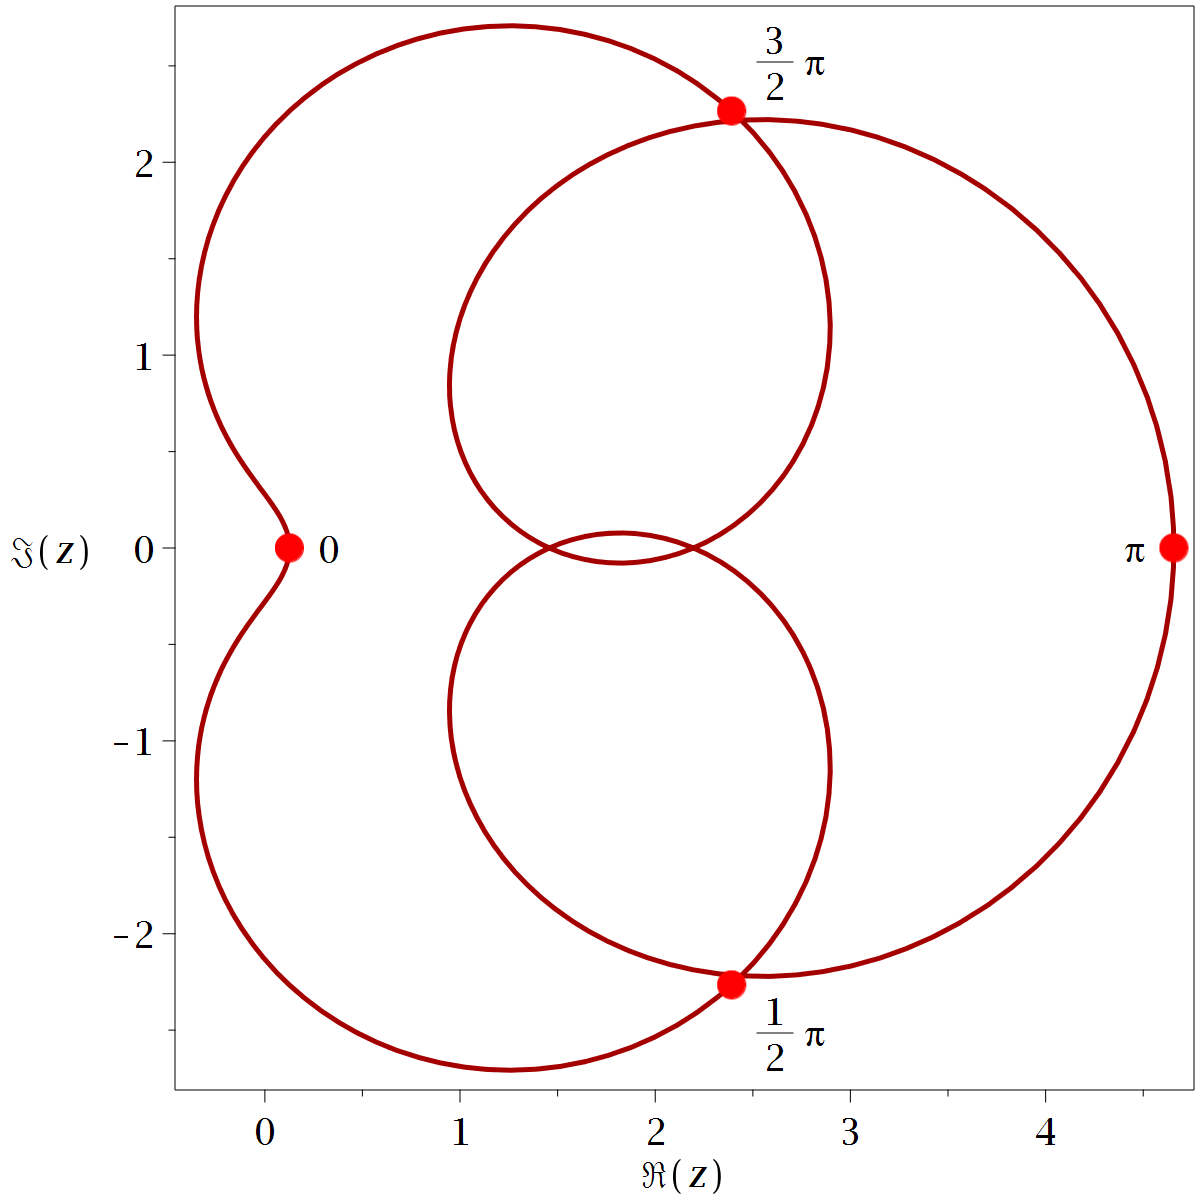
\includegraphics[width=0.45\textwidth]{CylinderU.png}
        \label{fig:u-cont}%
    }
    \hspace{1cm}
    \subfloat[The right hand side of (\ref{eq:branch-cut-issue}).]{%
        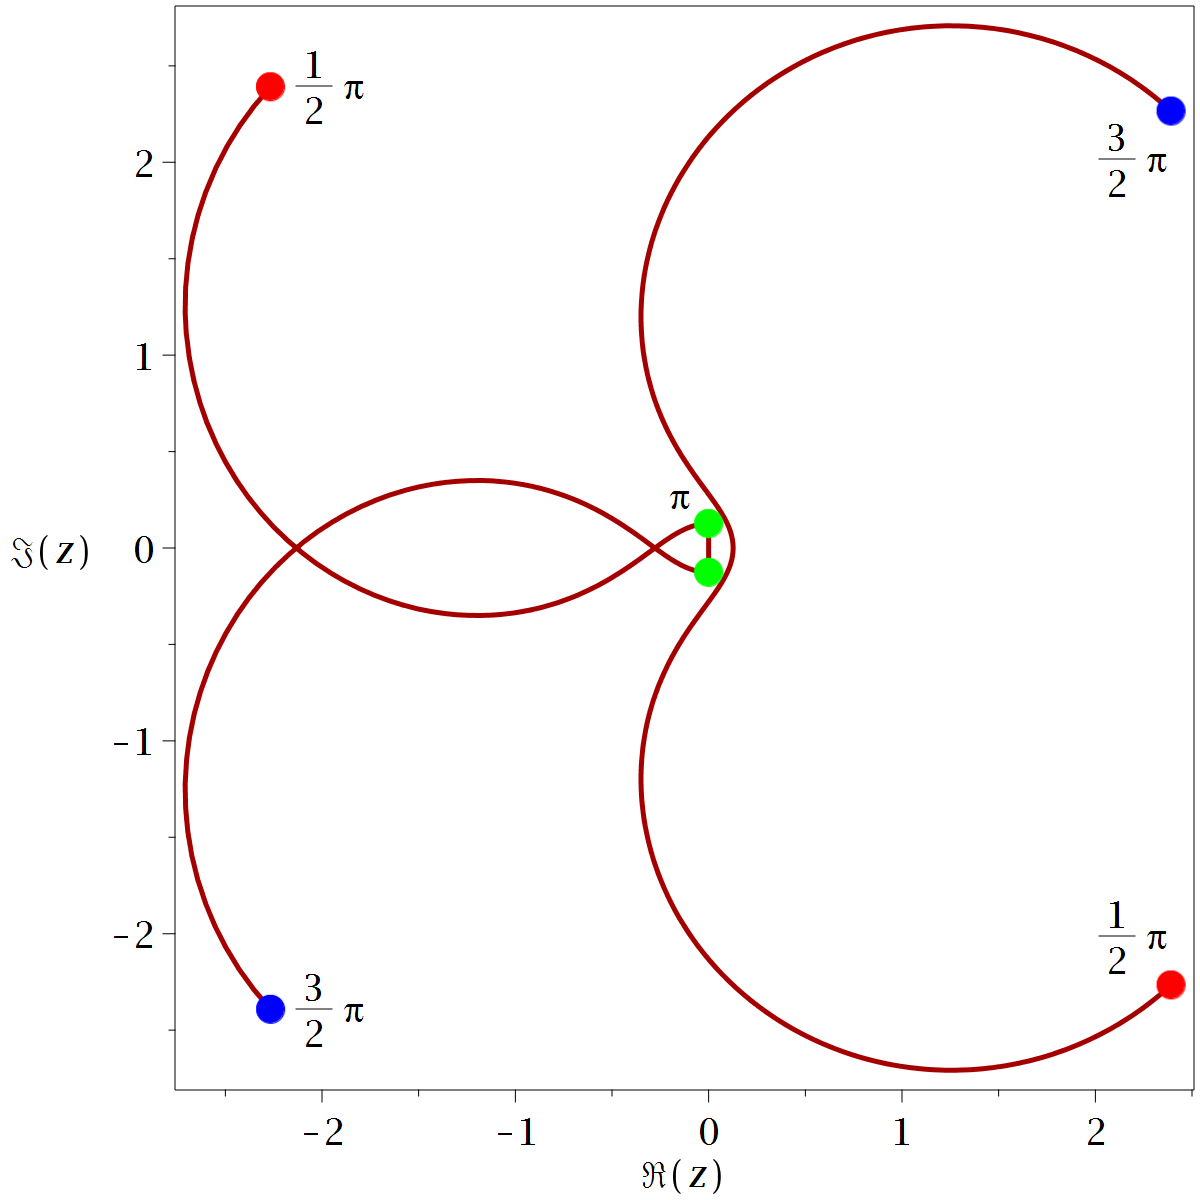
\includegraphics[width=0.45\textwidth]{WithCuts.png}
        \label{fig:bessel-cut}%
    }
    \caption{Two polar plots with $z=2.5\expe^{\iunit\phi}$ for $\phi \in [0,2\cpi]$ of left and right hand side of (\ref{eq:branch-cut-issue}) in \Maple. $U$ is an entire function, while $K_\nu$ and the square root function have a branch cut along $(-\infty,0]$. The colored dots represent the jumps over the branch cuts.}
    \label{fig:u-bessel}
\end{figure}

Since \gls{cas} do not provide Riemann surfaces, we use another approach to solve this problem, called \textbf{analytic continuation}. Analytic continuation is the process of extending the range of validity of a representation or more generally extending the region of definition of an analytic function~\parencite[152]{ComplexVariables}. For the modified Bessel function of the second kind the analytic continuation is defined in the \gls{dlmf}~\parencite[(10.34.4)]{NIST:DLMF}. With analytic continuation, the right hand side of equation~(\ref{eq:branch-cut-issue}) is illustrated in figure~\ref{fig:analytic-cont}.

\begin{figure}[!ht]
    \centering
    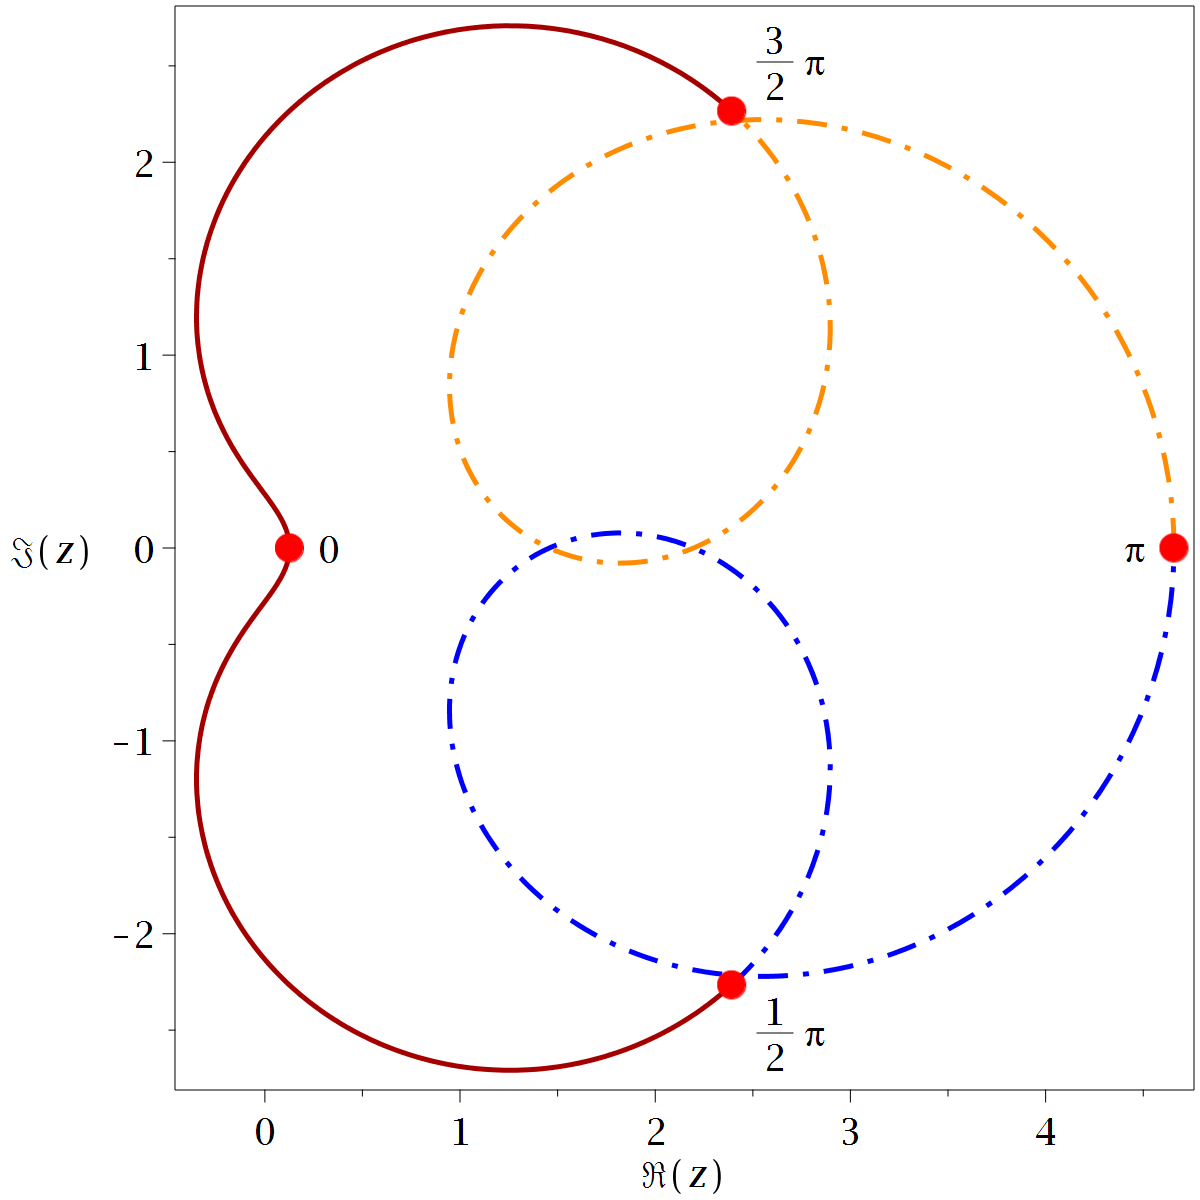
\includegraphics[width=0.6\textwidth]{WithAnalyticCont.png}
    \caption{The right hand side of (\ref{eq:branch-cut-issue}) using analytic continuation, when the function jumps over the branch cut at $\phi = \left\{\frac{\cpi}{2},\cpi\right\}$. At $\phi = \frac{3\cpi}{2}$, the function jumps back to the principal branch.}
    \label{fig:analytic-cont}
\end{figure}

\subsection{Injective, Surjective \& Bijective Mappings}
Later in the thesis, we will define our translation as a function. Since our main goal is to provide bijectivity for our translation, we will briefly introduce the terminology.

Consider a function $f: X \mapsto Y$.

\begin{definition}[Injective Function]
The function $f$ is \textbf{injective} if
\begin{equation}
\forall x,x' \in X: \quad f(x) = f(x') \Rightarrow x = x'.
\end{equation}
\end{definition}

\begin{definition}[Surjective Function]
The function $f$ is \textbf{surjective} if
\begin{equation}
\forall y \in Y, \exists x \in X: \quad y = f(x).
\end{equation}
\end{definition}

\begin{definition}[Bijection]
The function $f$ is \textbf{bijective} if $f$ is injective and surjective.
\end{definition}

The most useful part about bijective mappings is that every bijective function $f$ has an inverse function $f^{-1}$. Consider a translation between two systems as a function that is bijective. Such a translation has an inverse function, or in other words backward translation. This would allow us to translate each expression in one system to the other and back again.

Obviously, such a translation is desirable. However, we will see that this goal is not achievable for all possible expressions. Even worse, we will see that our translation is neither injective nor surjective.

\subsection{Graphs and Trees}
\glsreset{dag}
A typical way to formalize the structure of mathematical expressions are trees. We will briefly introduce what trees are and what an expression tree is.

\begin{definition}[Graph]
A \textbf{graph} is an ordered pair $G=(V,E)$, where $V$ is the set of \textbf{vertices} (or \textbf{nodes}) and $E$ the set of \textbf{edges}, which are a 2-element subset of $V$.
\end{definition}

\begin{definition}[Directed Graph]
A \textbf{directed graph} (sometimes also referred as \textbf{digraph}) $G = (V,E)$ is a graph with oriented edges. That means $E$ is a set of ordered pairs of vertices. Therefore, a graph is \textbf{undirected} if all edges $e \in E$ have no orientation.
\end{definition}

\begin{definition}[Paths, Cycles and connected Graphs]
Let $G = (V,E)$ be a directed or undirected graph with at least three vertices ($|V| \geq 3$). A \textbf{path} from one vertex $i\in V$ to another $j\in V$ is a finite sequence of vertices and edges
\begin{equation}
i = i_1, (i_1, i_2), i_2, \ldots , i_{k-1}, (i_{k-1}, i_k), i_k = j.
\end{equation}
A path is a \textbf{cycle} if $i = j$. If a graph $G = (V,E)$ has no cycles, it is called \textbf{acyclic}. Furthermore, if there is a path for every pair of vertices, $G$ is called \textbf{connected}.
\end{definition}

A \gls{dag}, for example, is used internally to represent mathematical expressions. However, another way to represent mathematical expressions are trees.

\begin{definition}[Tree]
A \textbf{tree} $T = (V,E)$ is an acyclic and connected graph.
\end{definition}

Let $T = (V,E)$ be a tree and $r \in V$. We call $r$ \textbf{root} of $T$ and order the other nodes in an ascending ordering according to its length of the path to $r$. Each node $v \in V$, which is directly connected with $r$ is called \textit{child} of $r$ and $r$ is called \textit{parent} of $v$. This can be defined for all nodes in the tree which created a hierarchical structure in the tree. A node is in a higher hierarchy, when it is closer to root node. A node can have multiple \textit{children}. Consider a node $a \in V$ as a node with three children $u,v,w$. We also define a order for the children, so that $u < v < w$. \textbf{Siblings} are nodes that share the same parent node. With the order we call $u$ the previous sibling of $v$ and $w$ the following sibling of $v$. With this additional terminology, we can move through trees easily. Trees with an ordering for all nodes and a root node are also called \textbf{ordered trees}.

Mathematical expressions can be represented by ordered trees consisting of terminal symbols, such as identifiers or numbers (leaf nodes), and functions or operators (non-leaf nodes)~\parencite{VMEXT}. Consider the mathematical expression
\begin{equation}\label{eq:simple-expr}
\expe^{x} + \frac{x^2}{\cpi}.
\end{equation}

The tool \gls{vmext}~\parencite{VMEXT} visualizes expression trees. Figure~\ref{fig:simple-expr-tree} draws the expression tree for (\ref{eq:simple-expr}).

\begin{figure}[ht]
    \centering
    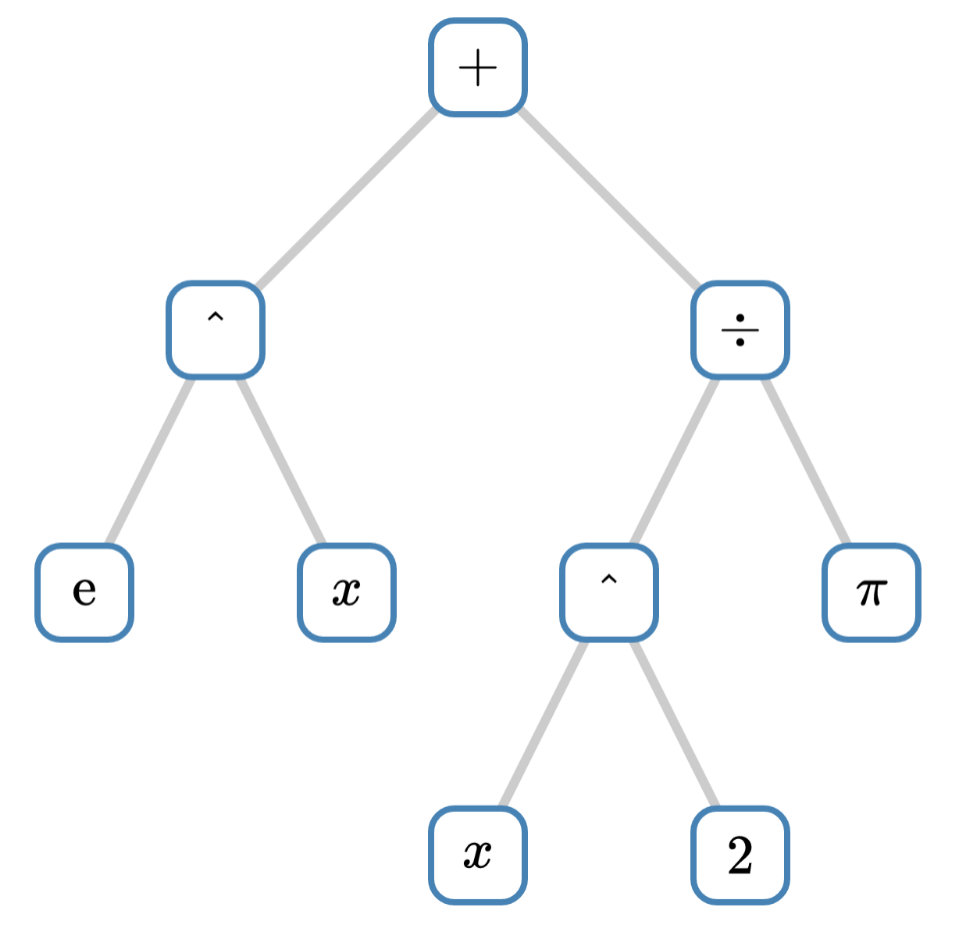
\includegraphics[width=0.7\textwidth]{expressionTreeSimple.png}
    \caption{The expression tree of (\ref{eq:simple-expr}) visualized with VMEXT~\parencite{VMEXT}.}
    \label{fig:simple-expr-tree}
\end{figure}
%\section{Digital Library of Mathematical Functions}\label{sec:dlmf}
\glsreset{dlmf}\glsreset{drmf}\glsreset{opsf}
The \gls{nist} \gls{dlmf}~\cite{NIST:DLMF:Paper} is the digital version of the \textit{NIST Handbook of Mathematical Function}. Internally, the \gls{dlmf} websites are \LaTeX{} files and all equations are numbered as usual. Therefore, we reference to a formula in the \gls{dlmf} with the given equation number.

The \gls{nist} \gls{drmf}~\cite{DRMF:14} is an outgrowth of the \gls{dlmf} and wants to create a digital compendium of mathematical formulae for \gls{opsf}. One of the main purposes is to facilitate interaction among a community of mathematicians and scientists~\cite{DRMF:15}. The \gls{drmf} also aims at expandability and interactivity. That was also a reason for this translation project, because a goal was to provide a one-click translation on the formulae in the \gls{drmf}.

Together, the \gls{dlmf} and \gls{drmf} build a comprehensive compendium for \gls{opsf} and they are therefore our main references in this thesis. A definition of a function in any \gls{cas} is therefore called different, if it differs from the corresponding \gls{dlmf}/\gls{drmf} definition.

%\section{Semantic \& Generic \LaTeX}\label{sec:semantics}
Donald E. Knuth developed the typesetting system \TeX{} in 1977~\cite[559]{DigitalTypo}, because he was unsatisfied with the typography of his book \textit{The Art of Computer Programming}, Volume 2~\cites[5]{DigitalTypo}{Knuth}. Around 1980, Leslie Lamport starts to extend \TeX{} by a set of macros, which became a new version of \TeX. According to his name \textit{Lamport}, this new version was called \LaTeX{~}\cite{LATEX}. Nowadays, \LaTeX{} has become the de facto standard for scientists to write their publications~\cite{LATEX:Standard}. This thesis, for example, is written in \LaTeXe, the current version of \LaTeX.

It is possible to customize and extend \LaTeX, for example through style files, where an editor can define new \LaTeX{} macros, environments and document styles.

\subsection{Mathematical Generic \LaTeX}
\LaTeX{} and \TeX{} enables printing of mathematical formulae in a structure similar to handwritten style. For example, the \LaTeX{} expression~\cite[(4.26.13)]{NIST:DLMF}
\begin{equation}\label{eq:latex-ex}
\verb|\int_{0}^{\infty} \sin(t^2) dt = \frac{1}{2} \sqrt{\frac{\pi}{2}}|
\end{equation}
will be rendered as
\begin{equation}\label{eq:latex-ex-r}
\int_{0}^{\infty} \sin(t^2) dt = \frac{1}{2} \sqrt{\frac{\pi}{2}}.
\end{equation}

We call the syntax of such mathematical expressions in \LaTeX{} \textit{mathematical \LaTeX{}} and hereafter use the terms \textit{\LaTeX{} expressions}, \textit{mathematical \LaTeX{} expressions} and \textit{mathematical \LaTeX{}} interchangeably.

Since \TeX{} and \LaTeX{} are typesetting systems, there are several ways to change the rendering of such mathematical expressions. However, for a \gls{cas} the information about the exact rendering of a mathematical expression is not as important as the meaning of the expression, the semantics.

\subsection{Semantic Information}\label{subsec:semantic-latex}
\textit{Semantics} in general is the study of meanings. Semantic information, for example, can be in words, whole sentences, mathematical expressions, and signs.

Consider the equation~(\ref{eq:latex-ex-r}). The meaning behind this expression is an equation. The left-hand side uses an infinite integral over the trigonometric sine function, which can be defined with~\cite[(4.14.1)]{NIST:DLMF}
\begin{equation}
\sin@{z} := \frac{\expe^{\iunit z}-\expe^{-\iunit z}}{2\iunit}.
\end{equation}
The right-hand side of~(\ref{eq:latex-ex-r}) contains a Greek letter $\cpi$, which is known to indicate the mathematical constant for the ratio of a circle's circumference to its diameter. However, $\pi$ can also indicate the prime-counting function. A human reader might conclude that $\pi$ cannot be the prime-counting function, because there is no variable given. In (\ref{eq:latex-ex-r}), $\cpi$ is much more likely the mathematical constant, also because the left-hand side contains the sine function and the mathematical constant $\cpi$ belonging to trigonometric functions.

As demonstrated, there are a lot of meanings behind~(\ref{eq:latex-ex-r}). Some of them are clear, others can be questionable. For a \gls{cas}, the exact meaning of a given input must be unique, otherwise the \gls{cas} cannot compute the input. Therefore, mathematical expressions in \gls{cas} contain accessible semantic information. This is realized to connect character sequences with unique internal procedures and classes, which represent specific mathematical objects.

Mathematical \LaTeX{} usually only contains information about the rendering of the expression and not about the meaning of the expression. However, there is semantic information in mathematical \LaTeX, but it's often hidden. This was shown in the example discussion of the meaning of equation~(\ref{eq:latex-ex-r}). In the plain text of the Greek letter $\pi$ (\verb|\pi|) is no exact meaning. Or, to be more precisely, there are multiple possible meanings, but there is no way to find the correct meaning. However, together with the left-hand side we can conclude that $\pi$ is the mathematical constant in that case. As demonstrated, there is semantic information in the expression, but a reader needs to analyze the whole expression and make conclusions to find it. Hence, for a computer it is difficult to understand mathematical \LaTeX. To provide a translation from mathematical \LaTeX{} to a \gls{cas}, the semantics must be clear and accessible.

We will introduce in the next subsection a semantic version of mathematical \LaTeX. To distinguish this version with classical mathematical \LaTeX, we call classical \LaTeX \textit{generic \LaTeX}.

Obviously, there must be different levels of semantics in expressions. We say an expression in generic \LaTeX{} such as 
\begin{equation}\label{eq:jac-latex}
\verb|P_n^{(\alpha,\beta)}(\cos(a\Theta))|
\end{equation}
contains less semantic information (more semantics are absent) than an appropriate representation in \Maple{}
\begin{equation}\label{eq:jac-maple}
\verb|JacobiP(n,alpha,beta,cos(a*Theta))|.
\end{equation}
This is because the meaning of (\ref{eq:jac-maple}) is unique and accessible, while the exact meaning of (\ref{eq:jac-latex}) must be concluded from the structure and context of the formula. Unfortunately, there is no formal definition for grading semantics or a \textbf{fully semantic} expression. However, we use this phrase, when there is sufficient semantic information accessible to provide an appropriate translation.

\subsection{DLMF/DRMF \LaTeX{} Macro Set}\label{subsec:macros}
Bruce Miller at \gls{nist} has created a set of semantic \LaTeX{} macros~\cite{DLMF:Macros}. Each macro ties specific character sequences to a well-defined mathematical object and is linked with the corresponding definition in the \gls{dlmf} or \gls{drmf}. Therefore, we call these semantic macros \Macro s. These semantic macros are internally used in the \gls{dlmf}, \gls{drmf} and also in this thesis. They are defined in multiple style files and allow optional parameters and multiple renderings. Table~\ref{tab:macro-def} show how a semantic macro is defined in a style file.

\begin{table}[ht]
\centering
\begin{tabular}{lp{7cm}}
	\hline
	\verb|\defSpecFun{function}| & Define a macro \verb|\function|.\\\hline
	\hspace*{0.5cm}\verb|[nparams]| & Number of parameters of the macro.\\\hline
	\hspace*{0.5cm}\verb|[optparams]| & The number of optional parameters of the macro.\\\hline
	\hspace*{0.5cm}\verb|{format}| & Defines the format of the macro. (How it will be displayed).\\\hline
	\hspace*{0.5cm}\verb|[keys]| & Attributes of the function. For example, \textit{meaning} or \textit{role}.\\\hline
	\hspace*{0.5cm}\verb|{arity}| & Number of arguments. Defines how many \{$\bullet$\} blocks come after the $@$ symbol.\\\hline
	\hspace*{0.5cm}\verb|[argformat]| & Format of arguments.\\\hline
	\hspace*{0.5cm}\verb|[altargformat]| & Alternative formats depends on the number of $@$ symbol.\\\hline
\end{tabular}
\caption{Overview for the definition of a semantic macro.}
\label{tab:macro-def}
\end{table}

The \verb|\defSpecFun| is a defined macro to easily define new macros for special functions. It takes a unique character sequence for the function name. The first optional argument \verb|nparams| defines the number of parameters of the special function. Some special functions, for example the associated Legendre functions, can define optional parameters. The general structure of a semantic macro has two parts to display the formula. The first part defines the display for the function symbol (including parameters) in \verb|{format}|. This format is fixed and cannot be changed. In contrast, the display for the arguments of the function can be controlled by the number of $@$ symbols and is defined in multiple optional \verb|[argformat]| blocks.

Consider the \textit{hypergeometric function}~\cite[(15.2.1)]{NIST:DLMF}. The semantic macro 
\begin{equation}
	\verb|\HypergeoF@{a}{b}{c}{z}| 
\end{equation}
is linked to the definition (15.2.1) in the \gls{dlmf}. The \textit{hypergeometric function} provides three different representations. Table~\ref{tab:hypergeo} gives an overview for all of them.

\begin{table}[ht]
\centering
\begin{tabular}{lc}
	\hline
	Semantic macro & Display\\
	\hline
	\tableRowSpace \verb|\HypergeoF@{a}{b}{c}{z}| & $\HypergeoF@{a}{b}{c}{z}$\\
	\tableRowSpace \verb|\HypergeoF@@{a}{b}{c}{z}| & $F\!\left({\genfrac{}{}{0pt}{}{a, b}{c}}; z \right)$\\
	\tableRowSpace \verb|\HypergeoF@@@{a}{b}{c}{z}| & $\HypergeoF@@@{a}{b}{c}{z}$\\
	\hline
\end{tabular}
\caption{The semantic macro for the \textit{hypergeometric function}~\cite[(15.2.1)]{NIST:DLMF} has three different ways to display the function. The different representations are controlled by the number of $@$ symbols.}
\label{tab:hypergeo}
\end{table}

The display of the function name $F$ is fixed, but the number of $@$ symbols control the display of the arguments. The third representation displays only the variable of the function, but hide the given parameters. Therefore, the semantic \LaTeX{} source in the background provide more semantic information than the displayed version. However, all of them represent the \textit{hypergeometric function} defined in the \gls{dlmf}.

The sets of macros from the \gls{dlmf} and the \gls{drmf} are mostly different. The \gls{drmf} uses the macros from the \gls{dlmf} and developed new macros as well. However, it happens that there are two different macros for the same mathematical object defined. One example is the \textit{Gegenbauer polynomial}\footnote{Also known as the \textit{ultraspherical polynomial}.}
\begin{eqnarray}
	&&\verb|\Ultra{\lambda}{n}@{x}|,\\
	&&\verb|\Ultraspherical{\lambda}{n}@{x}|.
\end{eqnarray}

There are currently 685 semantic macros defined. Note that the number of macros is constantly changing, because the project of semantic macros is still work in progress.

\subsection{Weakness of DLMF/DRMF Macros}\label{subsec:semanticVSmacro}
The set of \Macro s gives the opportunity to semantically enhance mathematical expressions. However, there are mostly macros for \gls{opsf}. It is difficult to foresee if a semantic macro provides sufficient semantic information for an appropriate translation, or, as we formulated above, if a semantic macro is really fully semantic.

One example is the \textit{Wronskian}. For example, for two differentiable functions the \textit{Wronskian} is defined as~\cite[(1.13.4)]{NIST:DLMF}
\begin{equation}
	\Wronskian@{w_1(z), w_2(z)} = w_1(z)w_2'(z) - w_2(z)w_1'(z).
\end{equation}
In semantic \LaTeX{} it is used with
\begin{equation}
	\verb|\Wronskian@{w_1(z), w_2(z)}|.
\end{equation}
It turned out, that for an appropriate translation to a \gls{cas}, we need access to the variables of $w_1(z)$ and $w_2(z)$. Therefore, we improved the macro and replaced it to a new version
\begin{equation}
	\verb|\Wron{z}@{w_1(z)}{w_2(z)}|.
\end{equation}
This new macro is displayed in the same way as the old version was displayed, but it provides more information. 

Another version of semantic \LaTeX{} is \sTeX, developed by Michael Kohlhase~\cite{sTeX}. This version of semantically enhanced \LaTeX{} is more comprehensive for general mathematics. It is not particularly useful for \gls{opsf}, and it doesn't link macros to unique mathematical definitions. Therefore, we did not use \sTeX{} in this project, although it provides more semantic information for simple arithmetic expressions. This part is almost completely missing in the \Macro s in its current state. One example is the question of white spaces. Scientists frequently uses white spaces to indicate multiplications. Most \gls{cas} are familiar with this convention and are able to understand such inputs. However, in \Maple's 1-D input notation, an asterisk is mandatory for multiplications. Therefore, we also added a macro \verb|\idot| (for \textit{invisible dot}), to provide a multiplication symbol which is not displayed in \LaTeX, but semantically enhances the \LaTeX{} expressions.
%\section{Computer Algebra Systems}\label{sec:cas}
\glsreset{cas}
A \gls{cas} is a mathematical software, which is, for example, able to analyze, simplify and compute mathematical expressions. It is based on the theory of computer algebra. Computer Algebra is a part of computer science that designs, analyzes, implements and applies algebraic algorithms~\cite{ComputerAlgebra}. In 1963, \textit{Schoonschip} was one of the first \gls{cas} developed by Martinus J. G. Veltman~\cite{Schoonschip}. It was mainly used for high-energy physics.

Using \gls{cas} was highly desirable, because it was a faster and easier alternative to calculation tables~\cite{Tables}. Another \gls{cas} \textit{MATLAB}\footnote{\textit{MATLAB} is an abbreviation for \textit{\textbf{mat}rix \textbf{lab}oratory}.} was initially developed by Cleve Moler in the late 1970s to allow students to use Fortran\footnote{Originally \textit{FORTRAN}, was the first widely used high-level programming language for general purposes and is still very popular for high-performance computing.} libraries without learning Fortran itself~\cite{MATLAB}. \textit{MATLAB} was constantly updated\footnote{Newest version is \textit{MATLAB 9.2} from march 2017.} and is still widely used for education and in image processing, because of its performance in linear algebra and numerical analysis.

Nowadays, there are several different \gls{cas} available. From proprietary solutions, such as \textit{MATLAB}, \Maple, \Mathematica, to freely available software packages, such as \textit{SageMath}. Most \gls{cas} are more or less specialized for fields in mathematics, such as \textit{MATLAB} for linear algebra and numerical computations. However, nowadays the most popular \gls{cas} are \Mathematica{} and \Maple.

\subsection{Maple}\label{subsec:maple}
\Maple{} was initially released in 1982 and is written in \textit{C}, \textit{Java} and its internal programming language, also called \textit{Maple}. The main purposes was to create an \gls{cas}, which would be able to run on lower cost computers. \Maple{} bases on a small kernel, which is written in \textit{C}, that provides the \Maple{} language. Additional libraries are written in the \Maple{} language, while the \gls{gui} is written in \textit{Java}.

In this thesis, we refer to version \textit{Maple 2016} and all information about internal data structures and the usage of \Maple{} is described in the manual~\cite{MAPLE:ProgrammingGuide}.

Internally, symbolic expressions are stored in the memory as \gls{dag} data structures. This avoids multiple blocks in the memory for the same object in an expression. 

Furthermore, \Maple{} allows different input notations: the \texttt{1D} input and the \texttt{2D} input. Consider the infinite integral
\begin{equation}\label{eq:maple-input}
\int\displaylimits_0^\infty \frac{\pi+\sin(2x)}{x^2} dx.
\end{equation}
The corresponding \texttt{1D} input notation in \Maple{} is
\begin{equation}\label{eq:1dmaple-input}
\texttt{int((Pi+sin(2*x))/x\^{}2, x=0..infinity)}.
\end{equation}

Historically, the \texttt{1D} format was used for inputting commands and expressions into \Maple, while the \texttt{2D} input is more used for interaction with human users. In fact, the internal \texttt{2D} representation is similar to \gls{mathML}~\cite{MathML} and its display is similar to \eqref{eq:maple-input}.

We consider \Maple's \texttt{1D} input as syntactically correct and our translation process always refers to the \texttt{1D} input representation rather than the \texttt{2D} input representation.

Another interesting characteristic, which becomes import for our translator, is determinism.

\begin{definition}[Deterministic Algorithm]
An algorithm is called \textbf{deterministic} if it produces always the same results on two identical inputs.
\end{definition}

\Maple{} is in general non-deterministic. That means, that two identical inputs possibly produce two different outputs depending on the run time environment. The reason is, that for example the order of the elements of a set\footnote{Mathematically, the elements in a set are not ordered. This is technically different in computer algebra, because each element is somewhere located in the memory. In a scope of a low-level programming environment, the elements of sets always have an order.} depends on the addresses of the elements in the memory. Mostly the background operation systems determine the positions of variables in the memory rather than the application \Maple{} does. 

However, \Maple{} works in sessions. When a user starts a worksheet a new \Maple{-session} will be created. It is also possible to start a new session in a worksheet with the command \texttt{restart}. Within such sessions \Maple{} is deterministic as long as the input doesn't use non-deterministic algorithms, such as probabilistic algorithms\footnote{Probabilistic algorithms use randomness to find approximate solutions. Such algorithms are obviously non-deterministic.}.

\subsection{Mathematica}\label{subsec:mathematica}
\textit{Wolfram Mathematica} was conceived by Stephen Wolfram and initially released in 1988~\cite{Mathematica}. It is also written in \textit{C/C++}, \textit{Java} and its internal programming language \textit{Wolfram Language}. It is one of the most comprehensive \gls{cas} nowadays and an ever growing software. The previously mentioned interactive document \gls{cdf} uses \Mathematica. Also the knowledge engine\footnote{Also known as answer engine, is a computer science discipline which tries to automatically answer questions posed by humans in natural language.} \textit{Wolfram|Alpha}\footnote{\url{https://www.wolframalpha.com/}, seen 08/2017} is based on \Mathematica.

In 2008 an error~\cite{Mathematica:Bug} in \Mathematica{} shows a problem of confidence in \gls{cas}. As we will explain later, our translator uses symbolic simplification\cite[section 2]{ComputerAlgebra} techniques in \Maple. Implemented symbolic simplification algorithms are rarely\footnote{In fact, there is no proof of correctness for symbolic simplifications in any \gls{cas} known.} proven and may therefore produce errors. We can only presume that the simplifications are correct.
%\section{Mathematical Language Processor}\label{sec:mlp}
\glsreset{mlp}\glsreset{pom}\glsreset{bnf}
The \gls{mlp}\footnote{Note that the official publication refers \gls{mlp} to \textit{Mathematical Language \textbf{Processor}}, rather than to the \textbf{parser}. However, the \textit{Mathematical Language Processor} project~\cite{MLP:Project} is slightly different and trying to analyize the natural language context of mathematical expressions. However, both projects are highly coupled and uses the same abbreviation. Since we focus on the parser, we use \gls{mlp} to refer to the \textit{Mathematical Language Parser}, even the official publication understood it as a \textbf{processor}.} project was developed to parse any mathematical expressions~\cite{POM-Tagger}. 

According to \gls{nlp}~\cite{NLP}, the \gls{mlp} understood mathematical expressions as a word of a formal language and parses expressions to so called parse trees. To understand the \gls{mlp}, we need to understand the concept of formal languages first. In the following, we will briefly introduce formal languages~\cite{Math:Encyclopedia:FormalLanguage}.

\begin{definition}[Alphabet]
An \textbf{Alphabet} $\Sigma$ is a finite, non-empty set. The elements of $\Sigma$ are called \textbf{letters} (or \textbf{symbols}).
\end{definition}

For example, the alphabet of a computer is simply the binary alphabet $\Sigma = \{1,0\}$.

\begin{definition}[Word]
A \textbf{word} (or string) $w$ over an alphabet $\Sigma$ is a finite sequence of letters of $\Sigma$. The set of all words over $\Sigma$ is denoted as $\Sigma^\ast$ (known as the Kleene star of $\Sigma$). The empty word $\epsilon$ (sequence of length 0) is always an element of $\Sigma^\ast$.
\end{definition}

\begin{definition}[Formal Language]
A subset $L \subseteq \Sigma^\ast$ is called \textbf{formal language} over an alphabet $\Sigma$.
\end{definition}

Hereafter we use the term \textit{formal language} and \textit{language} interchangeably. Usually, a formal language is constructed by a set of rules. In our case we construct a formal language by a context-free grammar~\cites[79]{Grammar}{IntroComp}.

\begin{definition}[Context-Free Grammar]
A context-free grammar $G = (V, \Sigma, R, S)$ is a $4$-tuple, where
\begin{enumerate}
\item $V$ is a finite set. The elements of $V$ are called \textbf{non-terminal symbols}.
\item $\Sigma$ is a finite set with $\Sigma \cap V = \varnothing$. The elements of $\Sigma$ are called \textbf{terminal symbols}.
\item $R$ is a finite relation from $V$ to $(\Sigma \cup V)^\ast$, thus $R \subseteq V \times (\Sigma \cup V)^\ast$. The members of $R$ are called \textbf{rules}.
\item $S \in V$ is called the \textbf{start symbol}.
\end{enumerate}
\end{definition}

A rule $(\alpha,\beta) \in R$ can be understood as a substitution. We denote the rule also as $\alpha \longrightarrow \beta$.

\begin{definition}[Derived Words \& Applied Rules]
Let $G = (V, \Sigma, R, S)$ be a context-free grammar. Let $A \in V$ and $u,v,w \in (\Sigma \cup V)^\ast$, such that $(A,w) \in R$. Than we say a word '$uwv$' can be \textbf{derived} in one step from the word '$uAv$' by \textbf{applying} the rule $(A,w)$.
\begin{equation}
uAv \Rightarrow uwv.
\end{equation}
\end{definition}

We can also apply multiple rules sequentially. 

\begin{definition}[Chain Derivation]
Let $G = (V, \Sigma, R, S)$ be a context-free grammar and $u,v \in (\Sigma \cup V)^\ast$, with $u \neq v$. We say $v$ can be derived from $u$, if
\begin{equation}
\exists\ k \geq 2\ \ \exists u_1, u_2, \ldots, u_k \in (\Sigma \cup V)^\ast: \quad u = u_1 \Rightarrow u_2 \Rightarrow \ldots \Rightarrow u_k = v,
\end{equation}
and write
\begin{equation}
u \overset{\ast}{\Rightarrow} v.
\end{equation}
\end{definition}

With a context-free grammar, we can define a context-free language over the grammar.

\begin{definition}[Context-Free Language]
Let $G = (V, \Sigma, R, S)$ be a context-free grammar. $G$ defines a language $L(G)$ by
\begin{equation}
L(G) = \left\{ w \in \Sigma^\ast:\ S \overset{\ast}{\Rightarrow} w \right\}.
\end{equation}
\end{definition}

A language $L$ is called \textbf{context-free language} if there is a grammar $G$, such that $L = L(G)$. In other words, a context-free language $L(G)$ is a set of all strings that can be derived from the start variable $S$ of $G$.

\begin{example}\label{ex:cfl}
A simple example for a context-free grammar are well-formed parentheses. Let $V = \{S\},\ \Sigma = \{(,\ )\}$ and $S$ be the start symbol. Furthermore, let $R$ contain the rules
\begin{eqnarray}
&&S \longrightarrow SS\\
&&S \longrightarrow (S)\\
&&S \longrightarrow ()
\end{eqnarray}
Let $G = (V, \Sigma, R, S)$. Than, for example
\begin{equation}\label{eq:example-proof}
\text{'}(()(()))\text{'} \in L(G).
\end{equation}
\end{example}

\begin{proof}[Proof of~\ref{eq:example-proof}]
We can produce the following chain of rules from $R$.
\begin{eqnarray}
S &\Rightarrow & (S)\label{eq:chain}\\
&\Rightarrow & (SS)\notag\\
&\Rightarrow & (()S)\notag\\
&\Rightarrow & (()(S))\notag\\
&\Rightarrow & (()(())).\notag
\end{eqnarray}
Therefore
\begin{equation}
S \overset{\ast}{\Rightarrow} \text{'}(()(()))\text{'} 
\end{equation}
and '$(()(()))$' $\in L(G)$.
\end{proof}

On the other hand
\begin{equation}
\text{'}(()\text{'} \not\in L(G).
\end{equation}

The chain of rules can also be represented in a tree structure. Such trees are called \textbf{parse trees}. The tree for~(\ref{eq:chain}) is visualized in figure~\ref{fig:parseTree}. Note that a parse tree is different to an expression tree. However, a parse tree can become an expression tree if the appropriated mathematical rules are defined.

\begin{figure}[ht]
	\centering
	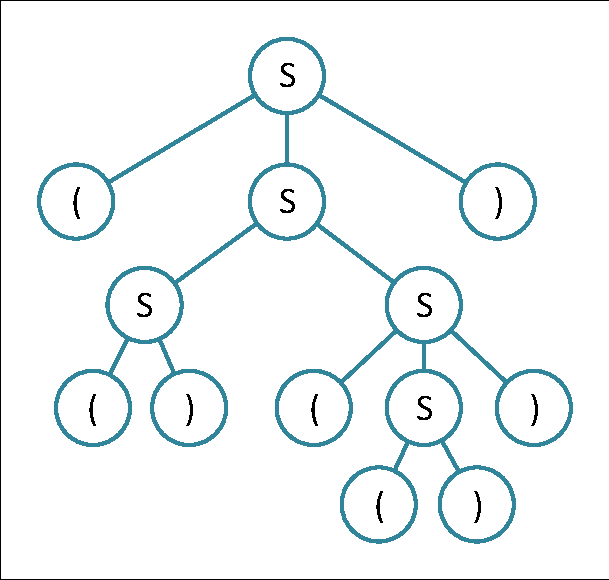
\includegraphics[clip, trim=0.2cm 0.2cm 0.2cm 0.2cm,width=0.6\textwidth]{ParseTree.pdf}
	\caption{The parse tree of the expression '$(()(()))$' for the well-formed parenthesis grammar $G = (V, \Sigma, R, S)$. Produced by the chain of rules~\ref{eq:chain}.}
	\label{fig:parseTree}
\end{figure}

There are several more definitions around formal languages, which we will not mention here. Note, for example, that a parse tree such as in figure~\ref{fig:parseTree} is not necessarily unique and can depend on the choice of a rule where more than one is \textit{applicable}. Consider a context-free grammar for simple arithmetic expressions with sums and subtractions of three variables $x,y$ and $z$. Let $V = \{S\},\ \Sigma = \{x,y,z,+,-\}$, $S$ be the start symbol and define the rules
\begin{eqnarray}
&&S \longrightarrow x\label{eq:chain-1}\\
&&S \longrightarrow y\label{eq:chain-2}\\
&&S \longrightarrow z\label{eq:chain-3}\\
&&S \longrightarrow S + S\label{eq:chain-4}\\
&&S \longrightarrow S - S\label{eq:chain-5}.
\end{eqnarray}
Now an expression such as $x+y-z$ is an element of the context-free language of $G = (V, \Sigma, R, S)$. However, there are two possible parse trees for this expression, tree~\ref{fig:parse1} and \ref{fig:parse2}, depending on the order of which rule gets applied first. Such grammars are also called ambiguous.

\begin{figure}[!ht]
    \centering
    \subfloat[The parse tree of $x+y-z$ if rule~(\ref{eq:chain-4}) gets applied first.]{%
        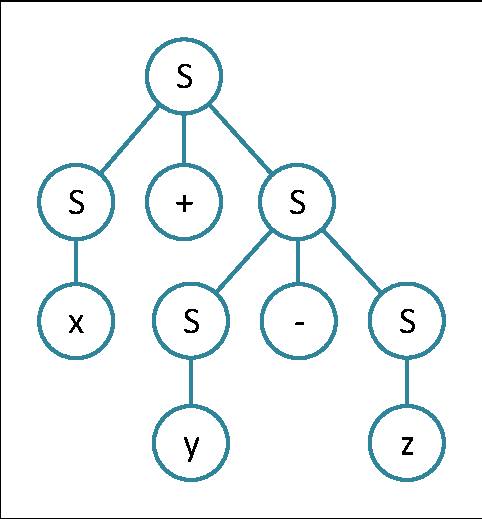
\includegraphics[clip, trim=0.2cm 0.2cm 0.2cm 0.2cm,width=0.4\textwidth]{ParseTree2a.pdf}
        \label{fig:parse1}%
    }
    \hspace{2cm}
    \subfloat[The parse tree of $x+y-z$ if rule~(\ref{eq:chain-5}) gets applied first.]{%
        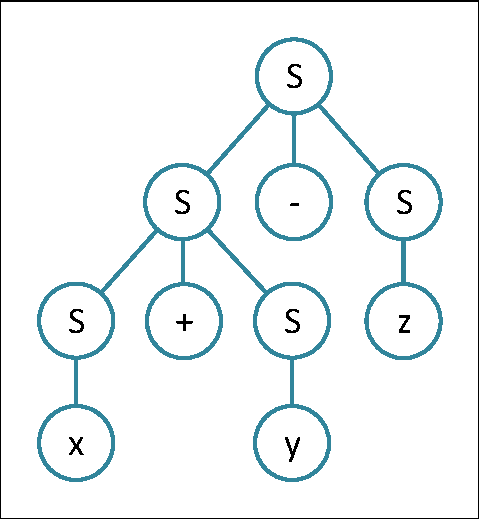
\includegraphics[clip, trim=0.2cm 0.2cm 0.2cm 0.2cm,width=0.4\textwidth]{ParseTree2b.pdf}
        \label{fig:parse2}%
    }
    \caption{Two different parse trees for $x+y-z$. \protect\subref{fig:parse1} applies rule~(\ref{eq:chain-4}) before (\ref{eq:chain-5}), while \protect\subref{fig:parse2} applies the rules vice versa.}
    \label{fig:parseMulti}
\end{figure}

A parser can define now in which order the rules get applied. For example, an \textbf{LL}-Parser parses the input from \textbf{L}eft to right and performing the \textbf{L}eftmost derivations. Leftmost in this terminology means, the parser takes the first applicable rule. In consequence, the internal ordering of rules is no longer irrelevant. The \gls{mlp} is such an \textbf{LL}-Parser. In case of the expression $x+y-z$ from above with the rules~(\ref{eq:chain-1}~-~\ref{eq:chain-5}), an \textbf{LL}-Parser would generates tree~\ref{fig:parse1}.

\subsection{BNF Grammar}
The \gls{bnf} is a notation technique for context-free grammars in computers. For example, a \gls{bnf} specification is a set of rules, written as
\begin{equation}
\verb|<symbol> ::= exp|,
\end{equation}
where \verb|<symbol>| is a non-terminal element and \verb|exp| are one or more sequences of symbols. Symbols that never appear on the left side are terminals.

The \gls{bnf} is often used to describe the syntax of programming languages. There are several tools that automatically generates a parser from a given grammar in \gls{bnf}. One of those tools is \textit{JavaCC} (for Java Compiler Compiler).

\subsection{POM-Tagger \& MLP}\label{subsec:pom-mlp}
The \gls{mlp} defines a \gls{bnf} grammar to parse mathematical \LaTeX{} expressions. The \gls{pom}-tagger (according to Part-of-Speech tagger in \gls{nlp}) categorizes math tokens. The main purpose of the \gls{pom}-tagger is the extraction of semantic information from mathematical \LaTeX. The \gls{pom} tagger is designed to perform multiple \textit{scans}. Given an input \LaTeX{} math document, the first scan of the tagger examines \textit{terms}, and groups them into sub-expressions where suitable. For instance $\verb|\frac{1}{2}|$ consists of two sub-expression of numerator and denominator. A \textit{term} is a non-terminal symbol defined in the \gls{bnf}. In the definition of a \LaTeX{} grammar this can be \LaTeX{} macros, environments, reserved symbols (such as the \LaTeX{} line break command \textbackslash\textbackslash), or numerical or alphanumerical expressions. The first scan of the \gls{pom}-tagger adds information to each term. The information is defined in lexicon files, which provide meanings, descriptions, categories and many more for a large variety of symbols. For example, table~\ref{tab:plus-lex-example} gives an example of the lexicon entry for the plus symbol.

\begin{table}[ht]
	\centering
	\begin{tabular}{lll}
	\hline
	\multicolumn{3}{l}{Symbol: \texttt{+}} \\
	\! & \multicolumn{2}{l}{Feature Set: universal} \\
	\! & \! & Category: operation\\
	\! & \! & Description: plus\\
	\! & \! & Source: unicode-math\\
	\! & \! & \TeX-equivalent: \verb|\mathplus|\\
	\! & \! & Unicode: u+0002b\\
	\hline
	\end{tabular}
	\caption{The lexicon entry for the $+$ symbol.}
	\label{tab:plus-lex-example}
\end{table}

A symbol can be tagged with multiple feature sets according to its ambiguous semantics. Tagged terms are called math terms. Math terms are rarely distinct at this stage and often have multiple features. All information are centralized in the \verb|global-lexicon.txt|.

Further scans will try to reduce the number of alternative feature sets by scanning the context of the math expression and concluding possible feature sets from the structure of the expression. See section~\ref{sec:resolution} for more information about this approach.

In its current state, the \gls{pom}-tagger only performs the first scan. Note that, technically, the \gls{mlp} parses mathematical expressions while the \gls{pom}-tagger categorizes elements of the parse tree. However, the \gls{mlp} also acts as an interface to interact with the parse tree and the \gls{pom}-tagger is a kind of an intermediate step of the whole parsing process. Therefore, we will refer to the \gls{mlp} in following chapters rather than to the \gls{pom}-tagger.

\subsection{MLP-Parse Tree}\label{subsec:mlp-syntax-tree}
Hereafter we consider the \gls{mlp-pt} as the parse tree, which is produced by the \gls{mlp}. The \gls{bnf} of the \gls{mlp} has no mathematical rules implemented in its current state. For example, there is no rule, similar to~(\ref{eq:chain-4}) for the binary operator $+$. Therefore, the \gls{mlp-pt} is not an expression tree. The \gls{pom} project was designed to extract semantic information from mathematical expressions. Certainly, the semantics of mathematical symbols is rarely unique. Consider the $-$ symbol as an example. As a binary operator it indicates the subtraction of two arguments. However, it is also a unary operator as a leading sign.

In its current stage, it is futile to implement arithmetical rules into the \gls{mlp} grammar. The next scan of the \gls{mlp} will reduce ambiguous meanings from the \gls{mlp-pt}. It can be anticipated that the \gls{mlp-pt} will become an expression tree when the planned next scans are implemented.

\begin{figure}[!ht]
    \centering
    \subfloat[The MLP-PT for $a+b$. The POM-Tagger adds information to all terminals. F-Set are feature sets. The terms $a$ and $b$ have multiple feature sets. An F-set represents another semantic meaning. In the figure are not all F-sets listed.]{%
        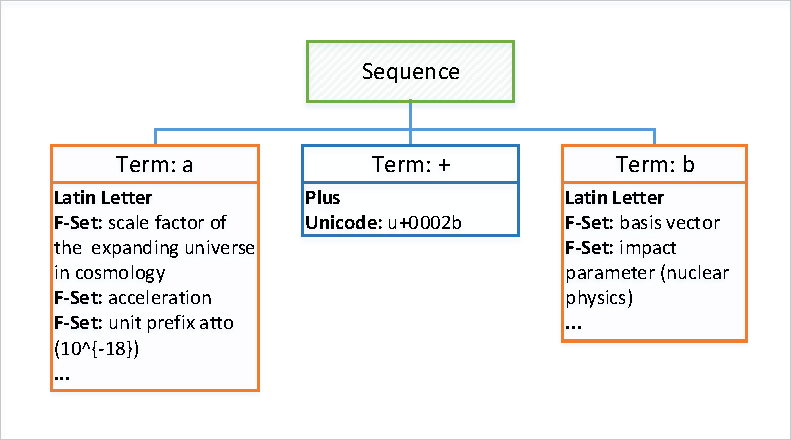
\includegraphics[clip, trim=0.2cm 0.2cm 0.2cm 0.2cm,width=0.65\textwidth]{ParseTreeSimple.pdf}
        \label{fig:tree-parse}%
    }
    \hspace{0.5cm}
    \subfloat[The expression tree for $a+b$.]{%
        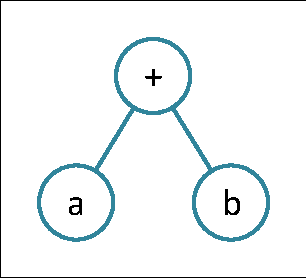
\includegraphics[clip, trim=0.2cm 0.2cm 0.2cm 0.2cm,width=0.25\textwidth]{ExpressionTreeSimple.pdf}
        \label{fig:tree-expr}%
    }
    \caption{Comparing the MLP-Parse tree with an expression tree for $a+b$.}
    \label{fig:tree-compare}
\end{figure}
%\section{Translator Definitions}\label{sec:definition}
To explain translations mathematically, we need to define some techniques first. Mainly, a translation process is a function that maps an input expression to an output expression. The input and output expressions are written in two different formal languages. For a translation, the exact types of input and output language are insignificant. Therefore, we consider mathematical \LaTeX, semantic \LaTeX, \Maple's \texttt{1D} input and \Mathematica{} input as formal languages. 

\begin{definition}[Translation]
Let $\mathcal{L}$ be a set of formal languages and $L_1, L_2 \in \mathcal{L}$ be two formal languages. A \textbf{translation} $\mathrm{tr}$ is a mapping from an input language $L_1$ to an output language $L_2$, denoted as
\begin{equation*}
\mathrm{tr}^{L_1}_{L_2}: L_1 \rightarrow L_2.
\end{equation*}
\end{definition}

\begin{definition}[Forward \& Backward Translation]
Let $\mathcal{L}$ be a set of formal languages. Let $L_1 \in \mathcal{L}$ be the language of semantic \LaTeX{} and $L_2 \in \mathcal{L}$ the language of any \gls{cas}. The function $\mathrm{tr}^{L_1}_{L_2}$ is called \textbf{forward translation to $L_2$} and $\mathrm{tr}^{L_2}_{L_1}$ is called \textbf{backward translation from $L_2$} respectively.
\end{definition}

Therefore, we define $\langTex$ as the formal language of semantic \LaTeX, $\langMaple$ as the formal language of \Maple{} and $\langMathe$ as the formal language of \Mathematica. Since we will only translate expressions between $\langTex$ and a \gls{cas}, we will use a more convenient notation for forward and backward translations. Let $t \in \langTex$ be an arbitrary expression in semantic \LaTeX{}. A forward translation to \Maple{} is denoted as
\begin{equation}
t \overset{\langMaple}{\mapsto} c, \quad \text{with } c \in \langMaple,
\end{equation}
and a backward translation from \Maple{} as
\begin{equation}
t \overset{\langMaple}{\mapsfrom} c, \quad \text{with } c \in \langMaple.
\end{equation}

Note that there is an identity translation between two formal languages $L_1, L_2$ defined if there is a word $w \in L_1 \cap L_2$. We specially denote the identity translation with 
\begin{align}
&\mathrm{id}^{L_1}_{L_2}:\ L_1 \rightarrow L_2,\notag\\
&\mathrm{id}^{L_1}_{L_2}(w) := w,\quad \text{with } w \in L_1 \cap L_2.
\end{align}

In this thesis, we will translate expressions from one system to another. There is no formal definition to compare mathematical expressions in two different systems. As an example, consider the trigonometric cosine function $\cos@{z}$. There is a formal definition in the \gls{dlmf} given~\cite[(4.14.2)]{NIST:DLMF}
\begin{equation}
\cos@{z} = \frac{\expe^{\iunit z} + \expe^{-\iunit z}}{2}.
\end{equation}
The internal definition of the cosine function in \Maple{} is given by
\begin{equation}
\cos@{z} = \frac{1}{2}\expe^{\iunit z} + \frac{1}{2\expe^{\iunit z}}.
\end{equation}
Technically, we would agree that both definitions are equivalent. However, \Maple{} is limited by the possibilities of a computer system. For example, the mathematical constant $\expe$ is irrational and can therefore never be \textit{absolutely equivalent} to the abstract mathematical construct of Euler's number. Instead of defining a new equivalence term for our purpose, we conveniently look for an \textbf{appropriate} translations between two formal languages. Obviously, this is not a formal definition, but should prevent us from translating one mathematical object\footnote{We are aware that it could be even more difficult to formally define what a \textit{mathematical object} is. We consider a mathematical object to be a function or symbol with a formal mathematical definition behind it.} into a completely different object in another language.

Therefore, we would label a translation such as
\begin{equation}\label{eq:cos-def}
\verb|\cos@{z}| \overset{\langMaple}{\mapsto} \verb|cos(z)|
\end{equation}
as \textit{appropriate}, while a translation such as
\begin{equation}
\verb|\cos@{z}| \overset{\langMaple}{\mapsto} \verb|sin(z)|
\end{equation}
would be \textit{inappropriate}. However, note that it is not always as easy as in this example to decide if a translation is appropriate or not. Therefore, we developed validation techniques to automatically check if a translation can be considered appropriate. In addition to this terminology, we introduce \textit{direct translations}. Later in the thesis, we will explain that a translation from one specific mathematical object to its \textit{appropriate} counterpart in the other system is not possible. We call a translation to the \textit{appropriate} counterpart \textbf{direct}. For example, the translation~(\ref{eq:cos-def}) is \textit{direct}, while a translation to the definition of the cosine function
\begin{equation}
\verb|\cos@{z}| \overset{\langMaple}{\mapsto} \verb|(exp(I*z)+exp(-I*z))/2|
\end{equation}
is not a \textit{direct} translation.
%\cleardoublepage

%\section{Semantic \LaTeX{} Translator}\label{ch:translator}
%\section{Translation Problems}\label{sec:problems}
There are several potential problems to perform translations between systems that embed semantic information in the input. Those problems vary from simple cases, e.g., a function is not defined in the system, too complex cases, e.g., different positioning of branch cuts for multivalued functions. This section will discuss the problems and workarounds.

If a function is defined in one system but not in the other, we can translate the definition of the mathematical function. For example, the \textit{Gudermannian}~\parencite[eq. 4.23.10]{NIST:DLMF} $\Gudermannian{x}$ function is defined by
\begin{equation}\label{eq:gudermannian}
\Gudermannian{x} := \atan{\sinh{x}} \quad x \in \Real.
\end{equation}
and linked with the semantic macro \verb|\Gudermannian| in the \gls*{dlmf} but does not exist in \Maple. We can perform a translation for the definition~\ref{eq:gudermannian} instead of macro itself
\begin{equation}\label{eq:guder-trans}
\verb|\Gudermannian{x}| \overset{\langMaple}{\mapsto} \texttt{arctan(sinh(x))}.
\end{equation}

Since those translations are nonintuitive, describing explanations become necessary for the translation process. A special logging function takes care of each translation and provide details after a successful translation process. Section~\ref{sec:forward-translation} explains this task further.

Providing detailed information also solves the problem for multiple alternative translations. In some cases, a semantic macro has two alternative representations in the \gls*{cas} or vice versa. In such cases, the translator picks one of the alternatives and informs the user about the decision.

In case of differences between defined branch cuts we can also use alternative translations to solve the problems. Consider the mentioned case of the arccotangent function~\parencite{Branches:acot} that has different positioned branch cuts in \Maple{} compared to the \gls*{dlmf} or \Mathematica{} definitions. Alternative but mathematically equivalent translations are
\begin{eqnarray}
\verb|\acot@{z}| & \overset{\langMaple}{\mapsto} & \verb|arccot(z)|,\label{eq:acot-alternatives}\\
& \overset{\langMaple}{\mapsto} & \verb|arctan(1/z)|,\label{eq:acot-alternatives-1}\\
& \overset{\langMaple}{\mapsto} & \verb|I/2*ln((z-I)/(z+I))|.\label{eq:acot-alternatives-2}
\end{eqnarray}

The direct translation~(\ref{eq:acot-alternatives}) has the branch cut issue, while the alternative translations~(\ref{eq:acot-alternatives-1}) and~(\ref{eq:acot-alternatives-2}) using other functions instead of the arccotangent function. The arctangent function~(\ref{eq:acot-alternatives-1}) and the natural logarithm~(\ref{eq:acot-alternatives-2}) have the same positioned branch cuts in the \gls*{dlmf} and in \Maple. In consequence, translation~(\ref{eq:acot-alternatives-1}) solves the issue, as long as the user do not evaulate the function at $z = 0$, while translation~(\ref{eq:acot-alternatives-2}) solves the issue except for $z = -\iunit$.

Other problematic cases for translations are the \Macro s itself. In some cases, they do not provide sufficient semantic information to perform translations. One example is the \textit{Wronskian} symbol. For two differentiable functions the \textit{Wronskian} is defined as~\parencite[eq. 1.13.4]{NIST:DLMF}
\begin{equation*}
	\mathscr{W} \left\{ w_1(z), w_2(z) \right\} = w_1(z)w_2'(z) - w_2(z)w_1'(z).
\end{equation*}
In semantic \LaTeX{} it is used with
\begin{equation}
	\verb|\Wronskian@{w_1(z), w_2(z)}|.
\end{equation}
A translation become infeasible, because the macro do not explicitely defined the variable of the functions $w_1$ and $w_2$. For a correct translation, the \gls*{cas} needs to be aware of the used variable $z$. We solved this issue by creating a new macro
\begin{equation}
	\verb|\Wron{z}@{w_1(z)}{w_2(z)}|.
\end{equation}
This example shows that the \Macro s are still work in progress and are getting constantly updated.

A similar problem is multiplications since they are rarely explicitly marked in \LaTeX{} expressions, e.g., scientists using whitespaces to indicate multiplications rather than using \verb|\cdot| or similar symbols. For such problems, we introduced a new macro \verb|\idot| for an invisible multiplication symbol (this macro will not be rendered). Since this macro is newly introduced and automatic conversion of existing equations is difficult, none of the equations in the \gls*{dlmf} uses this macro yet. As a consequence, the translator has some simple rules to perform translations without explicitly marked translations with \verb|\idot|.

Even we only allow the special dialect of \LaTeX{} using semantic macros not all expressions are unambiguous. In table~\ref{tab:amb-latex} are four examples of ambiguous expressions. These expressions are unambiguous for the \LaTeX{} compiler since it only considers the very next token for power and subscripts. Our translator following the same rules to solve these issues.

\begin{table}[ht]
\centering
\begin{tabular}{cc}
	\hline
	Ambiguous Input & \LaTeX{} Output\\
	\hline
	\verb|n^m!| & $n^m!$\\
	\verb|a^bc^d| & $a^bc^d$\\
	\verb|x^y^z| & Double superscript error\\
	\verb|x_y_z| & Double subscript error\\
	\hline
\end{tabular}
\caption{Ambiguous \LaTeX{} expressions and how \LaTeX{} displays them.}
\label{tab:amb-latex}
\end{table}

Another more questionable translation decision is alphanumerical expressions. As explained in table~\ref{tab:allTypesTable}, the \gls*{pom}-tagger handles strings of letters and numbers differently, depending on the order of the symbols. The reason is, that an expression such as '$4b$' is usually considered to be a multiplication of $4$ and '$b$,' while '$b4$' looks like indexing '$b$' by $4$. While the first example produces two nodes, namely $4$ and '$b$', the second example '$b4$' produces just a single alphanumerical node in the \gls*{pom-pt}. The translator interprets alphanumerical expressions as multiplications for two reasons. (1) We would assume that the inputs '$4b$' and '$b4$' are mathematically equivalent and (2) it is more common in mathematics to use single letter names for variables~\parencite{Notation:History}. Therefore we define the following definitions

\begin{eqnarray*}
\verb|4b| & \overset{\langMaple}{\mapsto} & \verb|4*b|,\\
\verb|b4| & \overset{\langMaple}{\mapsto} & \verb|b*4|,\\
\verb|energy| & \overset{\langMaple}{\mapsto} & \verb|e*n*e*r*g*y|.
\end{eqnarray*}

In general, the translator is drafted to solve ambiguous expressions or automatically find a work-around to disambiguate the expression. Only if there is no way to solve the ambiguity with the defined rules, the translation process stops.

\section{The Translator}
All translations are defined by a library (\gls*{csv} and \gls*{json} files) that defines translation patterns for each function and symbol. The pattern uses \verb|$i| as placeholders to define the positions of the arguments. For example, the translation patterns for the Jacobi polynomial are illustrated in table~\ref{tab:placeholder_ex2}.

\begin{table}[ht]
	\centering
	\begin{tabular}{lc}
		\hline
		\multicolumn{2}{l}{\textit{Forward Translation:}} \\
		\Maple & \verb|JacobiP($2, $0, $1, $3)| \\
		\Mathematica & \verb|JacobiP[$2, $0, $1, $3]|\\
		\hline
		\multicolumn{2}{l}{\textit{Backward Translation from \Maple/\Mathematica:}} \\
		Semantic \LaTeX & \verb|\JacobiP{$1}{$2}{$0}@{$3}|\\
		\hline
	\end{tabular}
	\caption{Forward and backward translation patterns of the Jacobi polynomial. The pattern for the backward translation is the same for \Maple{} and \Mathematica.}
	\label{tab:placeholder_ex2}
\end{table}

These placeholders causes trouble when the \gls*{cas} uses the symbol \verb|$| for other reasons, e.g., the differentiation in \Maple{} is defined by
\begin{equation*}
\verb|diff(f, [x$n])|,
\end{equation*}
where $f$ as an algebraic expression or an equation, $x$ the name of the differentiation variable and $n$ for the $n$-th order differentiation. A translation for $\frac{d^2x^2}{dx^2}$ should be like this
\begin{equation*}
\verb|\deriv[2]{x^2}{x}| \overset{\langMaple}{\mapsto} \verb|diff(x^2, [x$2])|
\end{equation*}
but would end up as
\begin{equation*}
\verb|\deriv[2]{x^2}{x}| \overset{\langMaple}{\mapsto} \verb|diff(x^2, [xx])|.
\end{equation*}

We can solve this issue by using paranthesis in such cases, e.g., \verb|diff($1, [$2$($0)])|.


The \Macro s also allow to specify optional arguments to distinguish between standard and another version of functions. The Legendre and associated Legendre function of the first kind are examples for such cases. The library that defines translations for each macro using the macro name as a primary key to identify the translation. The Legendre and associated Legendre function of the first kind both using the same macro \verb|\LegendreP|. To distinguish such cases, we are using a special syntax such cases, shown in table~\ref{tab:legendreP-lex}.

\begin{table}[ht!]
	\centering
	\begin{tabular}{ll}
		\hline
		Semantic Macro Entry & Maple Entry \\
		\hline
		\verb|\LegendreP{\nu}@{x}| & \verb|LegendreP($0, $1)| \\
		\verb|X1:\LegendrePX\LegendreP[\mu]{\nu}@{x}| & \verb|LegendreP($1, $0, $2)|\\
		\hline
	\end{tabular}
	\caption{Example entries of the Legendre and associated Legendre function in the translation library. The prefix notation \texttt{X<d>:<name>X} defines the translation for \texttt{<name>} with \texttt{<d>}-number of optional arguments.}
	\label{tab:legendreP-lex}
\end{table}

The translator using the \gls*{pom}-Tagger~\parencite{POM-Tagger}\footnote{Named according to the Part-of-Speech-Taggers in \gls*{nlp}.} to parse \LaTeX{} expressions into a parsed tree. The \gls*{pom}-Tagger is an \texttt{LL}-Praser defined by a context-free grammar in \gls*{bnf}. Each token will be tagged by meta information defined in lexicon files. We extend the lexicon files to provide also the information that is necessary for the translation process. An example of an entry of the lexicon file is given in table~\ref{tab:sine-lex-example}.

\begin{table}[ht!]
	\centering
	\begin{tabular}{lll}
	\hline
	\multicolumn{3}{l}{Symbol: \texttt{\textbackslash sin}} \\
	\! & \multicolumn{2}{l}{Feature Set: dlmf-macro} \\
	\! & \! & DLMF: \verb|\sin@@{z}|\\
	\! & \! & DLMF-Link: dlmf.nist.gov/4.14\# E1\\
	\! & \! & Meanings: Sine\\
	\! & \! & Number of Parameters: 0\\
	\! & \! & Number of Variables: 1\\
	\! & \! & Number of Ats: 2\\
	\! & \! & Maple: \verb|sin($0)|\\
	\! & \! & Maple-Link: www.maplesoft.com/support/\\
	\! & \! & \hspace{32pt} help/maple/view.aspx?path=sin\\
	\! & \! & Mathematica: \verb|Sin[$0]|\\
	\! & \! & Mathematica-Link: reference.wolfram.com/\\
	\! & \! & \hspace{32pt} language/ref/Sin.html\\
	\hline
	\end{tabular}
	\caption{The entry of the sine function in the lexicon file.}
	\label{tab:sine-lex-example}
\end{table}
%\section{Forward Translations}\label{sec:forward-translation}
An abstract translator class analyzes each node of the parsed tree and delegates them to specialized subtranslators. In this process, an object called \gls*{teo} is built. This \gls*{teo} is needed to rebuild a string representation of the mathematical expression after all nodes of the parsed tree were translated.

The parsed tree generated by the \gls*{pom}-tagger is not a mathematical expression tree. The \gls*{pom} project aims to disambiguate mathematical \LaTeX{} expressions and generates an expression tree. However, in the current state, many expressions cannot be disambiguated yet. In consequence, the \gls*{pom}-tagger generates a raw parsed tree where each token in the \LaTeX{} expression is a node in the tree. We call this parsed tree, the \gls*{pom-pt}.

{\sloppy The overall forward translation process is explained in~\Cref{fig:forward-trans}. All translation patterns and related information are stored in the DLMF/DRMF tables. These tables are converted by the \verb|lexicon-creator| to the \verb|DLMF-macros-lexicon| lexicon file. Together with the \verb|global|-\verb|lexicon| file, the \gls*{pom-pt} will be created by the \gls*{pom}-tagger. The \verb|latex-converter| takes a string representation of a semantic \LaTeX{} expression and uses the \gls*{pom} engine as well as our \verb|Translator| to create an appropriate string representation for a specified \gls*{cas}.}

\begin{figure}[ht]
	\vspace{-10pt}
	\centering
	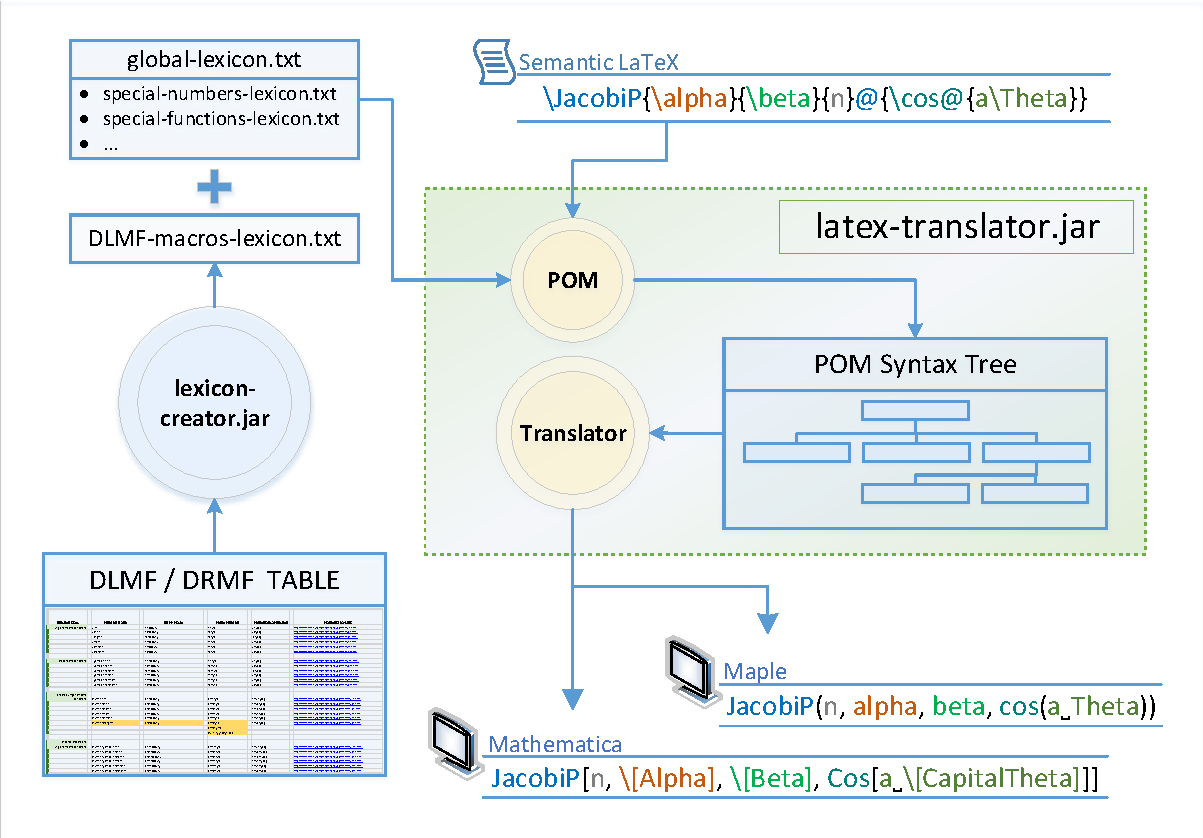
\includegraphics[clip, trim=0.2cm 0.2cm 0.2cm 0.2cm, scale=0.72]{ForwardTranslationProcess.pdf}
	\caption{Process diagram of a forward translation process. The \gls*{pom}-tagger generates the \gls*{pom-pt} based on lexicon and \gls*{json} files. The \gls*{pom-pt} will be translated to different \gls*{cas}.}
	\label{fig:forward-trans}
	\vspace{-10pt}
\end{figure}

\subsection{Analyzing the PoM-Parsed Tree}\label{subsec:analyze-mlp}
Since the \gls*{bnf} does not define rules for semantic macros, each argument of the semantic macro and each $@$ symbol are following siblings of the semantic macro node. That is the reason why we stored the number of parameters, variables and $@$ symbols in the lexicon files. Otherwise, the translator could not find the end of a semantic macro in the \gls*{pom-pt}.

\begin{figure}[ht]
	\centering
	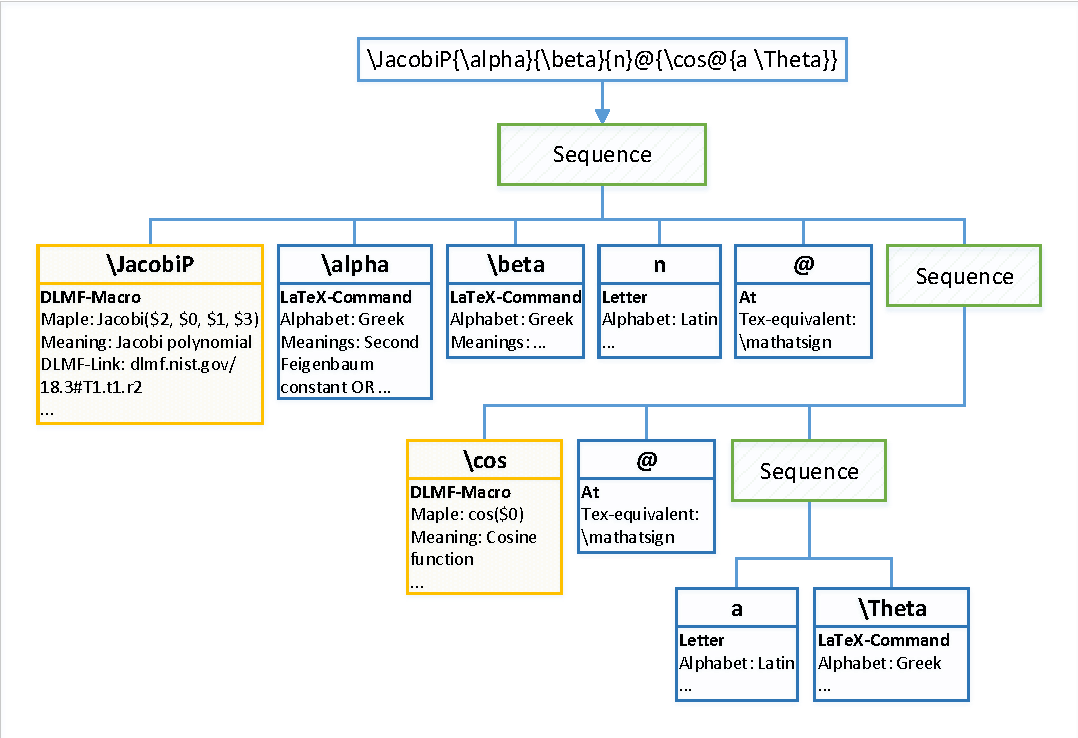
\includegraphics[clip, trim=0.2cm 0.2cm 0.2cm 0.2cm, scale=0.75]{SyntaxTreeUseCase.pdf}
	\caption{The \gls*{pom-pt} for the Jacobi polynomial example~\eqref{eq:P} using the DLMF/DRMF \LaTeX{} macro. Each leaf contains information from the lexicon files.}
	\label{fig:syntax-tree-usecase}
	\vspace{-10pt}
\end{figure}

\begin{wrapfigure}{r}{0.5\textwidth}
\vspace{-20pt}
\begin{minipage}{0.5\textwidth}
\begin{algorithm}[H]
\caption{Simple translation algorithm for the POM-Parse Tree}\label{alg:simple-translation}
	\begin{algorithmic}[1]
	\Require Root $r$ of the parse tree $T$
	\Procedure{translate}{$r$}
	\If{$r$ is leaf}
		\State {\scriptsize TRANSLATE\_LEAF}($r$);
	\Else
		\ForAll{children $v_n$ of $r$}
			\State {\scriptsize TRANSLATE}($v_n$);
		\EndFor
	\EndIf
	\EndProcedure
	\end{algorithmic}
\end{algorithm}
\end{minipage}
\vspace{-14pt}
\end{wrapfigure}

\Cref{fig:syntax-tree-usecase} visualizes the \gls*{pom-pt} of the Jacobi polynomial example from~\Cref{tab:JacobiP-usecase}. Because of the differences to expression trees, a backward conversion of the \gls*{pom-pt} to a string representation can be difficult, especially for finding necessary or unnecessary parentheses. Therefore we create the \gls*{teo}.

With these tools, we can translate a \LaTeX{} expression by translating the \gls*{pom-pt} node by node and perform group or reordering operations for some special cases. The algorithm is realized in a simple recursive structure. The Algorithm~\ref{alg:simple-translation} explains the translation process. Whenever the algorithm finds a leaf, it can translate this single term. If the node is not a leaf, it starts to translate all children of the node recursively. 

\begin{algorithm}[t]
\caption{Abstract translation algorithm to translate MLP-Parse trees.}\label{alg:translation}
	\begin{algorithmic}[1]
	\Require Root $r$ of a POM-Parse tree $T$. List \textit{following\_siblings} with the following siblings of $r$. The list can be empty.
	\Procedure{abstract\_translator}{$r$, \textit{following\_siblings}}
	\If{$r$ is leaf}
		\State {\scriptsize TRANSLATE\_LEAF}($r$, \textit{following\_siblings});\label{line:transLeaf}
	\Else
		\State \textit{siblings} $ = r$.getChildren(); \Comment{\textit{siblings} is a list of children}
		\State {\scriptsize ABSTRACT\_TRANSLATOR}(\textit{siblings}.removeFirst(), \textit{siblings});\label{line:transSeq}
	\EndIf
	\If{\textit{following\_siblings} is not empty}\label{line:ifNotEmpty}
		\State $r =$ \textit{following\_siblings}.removeFirst();
		\State {\scriptsize ABSTRACT\_TRANSLATOR}($r$, \textit{following\_siblings});
	\EndIf
	\EndProcedure
	\end{algorithmic}
\end{algorithm}
%\vspace{-20px}

This approach is not completely feasible since the algorithm needs to look ahead and check the following siblings in some cases, e.g., in the case of a semantic macro with arguments (see~\Cref{fig:syntax-tree-usecase}). The {\footnotesize \verb|TRANSLATE_LEAF|} function needs to know the following siblings of the current node. Algorithm~\ref{alg:translation} explains a more detailed but abstract version of the final algorithm of the presented translation tool. 

If the root $r$ is a leaf, it still can be translated as a leaf. Eventually, some of the following siblings are needed to translate $r$. The list of \textit{following\_siblings} in Line~\ref{line:transLeaf} might be reduced to avoid multiple translations for one node. If $r$ is not a leaf, it contains one or more children. Therefore, we can call the {\footnotesize \verb|ABSTRACT_TRANSLATOR|} recursively for the children. Once we have translated $r$, we can go a step further and translate the next node. Line~\ref{line:ifNotEmpty} checks if there are following siblings left and calls the {\footnotesize \verb|ABSTRACT_TRANSLATOR|} recursively in such cases. Translated expressions are stored by the \gls*{teo} object. Algorithm~\ref{alg:translation} is a simplified version of the translator process. The \Cref{line:transLeaf,line:transSeq} process the translations for each node. \Cref{tab:allTypesTable} gives an overview of all the different node types the root $r$ can be. A more detailed explanation of the types can be found in~\parencite{POM-Tagger}.

The \gls*{bnf} grammar defines some basic grammatical rules for generic \LaTeX{} macros, such as for \verb|\frac|, \verb|\sqrt|. Therefore, there is a hierarchical structure for those symbols similar to the structure in expression trees. As already mentioned, some of these types can be translated directly, such as Greek letters, while others are more complex, such as semantic \LaTeX{} macros. Therefore, the translators delegate the translation to specialized subtranslators. This delegation process is implemented in \Cref{line:transLeaf,line:transSeq} of Algorithm~\ref{alg:translation}. The Subsection~\ref{sec:subtranslators} discusses these classes in more detail.

\begin{table}[H]
\vspace{-10pt}
\centering
\sloppy
\newcolumntype{L}{>{\raggedright\arraybackslash}X}
\newcolumntype{Y}[1]{>{\raggedright\let\newline\\\arraybackslash\hspace{0pt}}p{#1}}
\begin{tabularx}{\textwidth}{Y{1.55cm} Y{2.5cm} L L}
	\hline
	& \textbf{Node type} & \textbf{Explanation} & \textbf{Example} \\
	\hline
	\hline
	\multicolumn{1}{Y{1.5cm}|}{\textbf{$r$ has children}} & Sequence & Contains a list of expressions. & $a+b$ is a sequence with three children ($a$, $+$ and $b$).\\
	\cline{2-4}
	\multicolumn{1}{l|}{} & Balanced Expression & Similar to a sequence. But in this case the sequence is wrapped by \texttt{\tbs left} and \texttt{\tbs right} delimiters. & \texttt{\tbs left(}$a+b$\texttt{\tbs right)} is a balanced expression with three children ($a$, $+$ and $b$).\\
	\cline{2-4}
	\multicolumn{1}{l|}{} & Fraction & All kinds of fractions, such as \texttt{\tbs frac}, \texttt{\tbs ifrac}, etc. & \texttt{\tbs ifrac\{a\}\{b\}} is a fraction with two children ($a$ and $b$).\\
	\cline{2-4}
	\multicolumn{1}{l|}{} & Binomial & Binomials & \texttt{\tbs binom\{a\}\{b\}} has two children ($a$ and $b$).\\
	\cline{2-4}
	\multicolumn{1}{l|}{} & Square Root & The square root with one child. & \texttt{\tbs sqrt\{a\}} has one child ($a$).\\
	\cline{2-4}
	\multicolumn{1}{l|}{} & Radical with a specified index & $n$-th root with two children. & \texttt{\tbs sqrt[a]\{b\}} has two children ($a$ and $b$).\\
	\cline{2-4}
	\multicolumn{1}{l|}{} & Underscore & The underscore '\_' for subscripts. & The sequence $a$\_$b$ has two children ($a$ and '\_'). The underscore itself '\_' has one child ($b$).\\
	\cline{2-4}
	\multicolumn{1}{l|}{} & Caret & The caret '\^{}' to for superscripts or exponents. Similar to the underscore. & The sequence $a$\^{}$b$ has two children ($a$ and '\^{}'). The caret itself '\^{}' has one child ($b$).\\
	\hline
	\hline
	\multicolumn{1}{Y{1.5cm}|}{\textbf{$r$ is a leaf}} & \Macro{} & A semantic \LaTeX{} macro & \texttt{\tbs JacobiP}, etc.\\
	\cline{2-4}
	\multicolumn{1}{l|}{} & Generic \LaTeX{} macro & All kinds of \LaTeX{} macros & \texttt{\tbs Rightarrow}, \texttt{\tbs alpha}, etc.\\
	\cline{2-4}
	\multicolumn{1}{l|}{} & Alphanumerical Expressions & Letters, numbers and general strings. & Depends on the order of symbols. $ab3$ is alphanumerical, while $4b$ are two nodes ($4$ and $b$).\\
	\cline{2-4}
	\multicolumn{1}{l|}{} & Symbols & All kind of symbols & '$@$', '$*$', '$+$', '$!$', etc.\\
	\hline
\end{tabularx}
\caption{A table of all kinds of nodes in a MLP syntax tree. Note that this table groups some kinds for a better overview. For a complete list and a more detailed version see~\cite{POM-Tagger}.}
\label{tab:allTypesTable}
\end{table}

This approach seems to work for most of semantic \LaTeX{} expressions. However, there is one problem with this straight forward approach which was mentioned shortly mentioned in~\Cref{sec:problems}. There are many different types of notations used to represent formulae. \Cref{tab:notations} illustrates the simple expression $(a+b)x$ in different notations. The \gls*{pol}\footnote{Also known as \textit{Warsaw Notation} or \textit{prefix notation}} (hereafter called prefix notation) places the operator to the left of/before its operands. The \gls*{rpol}\footnote{Also known as \textit{postfix notation}} (hereafter called postfix notation) does the opposite and places the operator to the right of/after its operands. The infix notation is commonly used in arithmetic and places the operator between their operands, which only makes sense as long as the operator is a binary operator.

\begin{wrapfigure}{r}{0.38\textwidth}
\vspace{-10pt}
\begin{minipage}{0.38\textwidth}
\center
\begin{tabular}{lc}
	\hline
	Notation & Expression \\
	\hline
	Infix & $(a+b) \cdot x$\\
	Prefix & $\cdot + a\ b\ x$\\
	Postfix & $a\ b + x\ \cdot$\\
	Functional & $\cdot(+(a, b), x)$\\
	\hline
\end{tabular}
\vspace{-5pt}
\caption{The mathematical expression '$(a+b) \cdot x$' in infix, prefix, postfix and functional notation.}
\label{tab:notations}
\end{minipage}
\vspace{-5pt}
\end{wrapfigure}

In mathematical expressions, notations are mostly mixed, depending on the case and number of operands. For example, infix notation is common for binary operators ($+$, $-$, $\cdot$, $\mod$, etc.), while functional notations are conveniently used for any kind of functions ($sin$, $cos$, etc.). Sometimes the same symbol is used in different notations to distinguish different meanings. For example, the `$-$' as a unary operator is used in prefix notation to indicate the negative value of its operand, such as in `$-2$'. Of course, `$-$' can also be the binary operator for subtraction, which is commonly used in infix notation. An example for the postfix notation is factorial, such as `$2!$'.

Most programming languages (and \gls*{cas} as well) internally use prefix or postfix notation and do not mix the notations in one expression, since it is more convenient to parse expressions in uniform notations. However, the common practice in science is to use mixed notations in expressions. Since the \gls*{pom} has rarely implemented mathematical grammatical rules yet, it takes the input as it is and does not build an expression tree. Therefore, it parses all four examples from~\Cref{tab:notations} to four different \gls*{pom-pt}s rather than to one unique expression tree. In general, this is not a problem for our translation process since most \gls*{cas} are familiar with the most common notations. Therefore, the translator does not need to know that `$a$' and `$b$' are the operands of the binary operator `$+$' in `$a+b$.' The translator could simply translate the symbols in `$a+b$' in the same order as they appear in the expression and the \gls*{cas} would understand it. However, this simple approach generates two problems.
\begin{enumerate}%[label=\arabic*)]
\item \label{prob:1} The translated expression is only syntactically correct if the input expression was syntactically correct.
\item \label{prob:2} We cannot translate expressions to a \gls*{cas} which uses a non-standard notation.
\end{enumerate}

Problem~\ref{prob:1} should be obvious. Since we want to develop a translation tool and not a verification tool for mathematical \LaTeX{} expressions, we can assume syntactically correct input expressions and produce errors otherwise. Problem~\ref{prob:2} is more difficult to solve. If a user wants to support a \gls*{cas} that uses prefix or postfix notation by default, the translator would fail in its current state. Supporting \gls*{cas} with another notation would be a part of future work.

Nonetheless, changing a notation could also solve ambiguities in some situations. Consider the two ambiguous examples in~\Cref{tab:amb_ex}. While a scientist would probably just ask for the right interpretation of the first example, \Maple{} automatically computes the first interpretation. On the other hand, \LaTeX{} automatically disambiguate the first example by only recognizing the very next element (single symbols or sequence in curly brackets) for the superscript and therefore displays the second interpretation. The second example is already interpreted as the double factorial function of $n$, since this notation is the standard interpretation in science. We wrote the second interpretation as the standard way in science to make it even more obvious. However, surprisingly, \Maple{} computes the first interpretation again rather than the common standard interpretation.
\begin{table}[ht]
\centering
\begin{tabular}{lccc}
	\hline
	& Text Format Expression & First Interpretation & Second Interpretation\\
	\hline
	1: & \rule{0pt}{0.9\normalbaselineskip} $4\ \hat{\ }\ 2!$ & $4^{2!}$ & $4^2!$ \\
	2: & $n!!$ & $(n!)!$ & $(n)!!$\\
	\hline
\end{tabular}
\caption{Ambiguous examples of the factorial and double factorial function. One expression in a text format can be interpreted in different ways.}
\label{tab:amb_ex}
\end{table}

In most cases, parentheses can be used to disambiguate expressions. We used them in~\Cref{tab:amb_ex} to clarify the different interpretations in example 2. But sometimes, even parentheses cannot solve a mistaken computation. For example, there is no way to add parentheses to force \Maple{} to compute `$n!!$' as the double factorial function. Even `$(n)!!$' will be interpreted as `$(n!)!$'. Rather than using the exclamation mark in \Maple, one could also use the functional notation. For example, the interpretations `$(2!)!$' and `$(2)!!$' can be distinguished in \Maple{} by using \verb|factorial(factorial(2))| and \verb|doublefactorial(2)| respectively. We define the translations as follows:

\begin{eqnarray*}
\verb|n!| &\overset{\langMaple}{\mapsto}& \verb|factorial(n)|,\\
\verb|n!!| &\overset{\langMaple}{\mapsto}& \verb|doublefactorial(n)|.
\end{eqnarray*}
%The translator needs to presume some properties for the functions similar to \LaTeX, which only recognizes the very next element right after the caret for the superscript. 

Algorithm~\ref{alg:translation} does not allow this translation right now. It has no access to previously translated nodes in its current state. This problem is solved by the \gls*{teo} that stores and groups translated objects like lists. This allows to access the latest translated expression and use it as the argument for the factorial function. Table~\ref{tab:teo-list} shows three example for the \gls*{teo} list that groups some tokens.

\begin{table}[ht]
\centering
\begin{tabular}{cc}
	\hline
	Input Expression & TEO List\\
	\hline
	$a+b$ & \verb|[a, +, b]|\\
	$(a+b)$ & \verb|[(a+b)]|\\
	$\frac{a}{b}-2$ & \verb|[(a)/(b), -, 2]|\\
	\hline
\end{tabular}
\caption{How the TEO-list groups subexpressions.}
\label{tab:teo-list}
\end{table}

\subsection{Subtranslators}\label{sec:subtranslators}

A \verb|SequenceTranslator| translates the \textit{sequence} and \textit{balanced expressions} in the \gls*{pom-pt}. If a node $n$ is a leaf and the represented symbol an open bracket (parentheses, square brackets and so on) the following nodes are also taken as a \textit{sequence}. Hence, combined with the recursive translation approach, the \verb|SequenceTranslator| also checks balances of parentheses in expressions. An expression such as `$(a]$' is producing a mismatched parentheses error. On the other hand, this is a problem for interval expressions such as `$[a,b)$'. In the current version, the program cannot distinguish between mismatched parentheses and half-opened, half-closed intervals. Whether an expression is an interval or another expression is difficult to decide and can depend on the context. Also, the parenthesis checker could simply be deactivated to allow mismatched parentheses in an expression. But this functionality is not implemented yet.

The \verb|SequenceTranslator| also handle positions of multiplication symbols. There are a couple of obvious choices to translate multiplication signs. The most common symbol for multiplications is still the white space or none symbol at all, as explained previously. Consider the simple expression `$2n\pi$'. The \gls*{pom-pt} generates a sequence node with three children, namely $2$, $n$ and $\pi$. This sequence should be interpreted as a multiplication of the three elements. The \verb|SequenceTranslator| checks the types of the current and next nodes in the tree to decide if it should add a multiplication symbol or not. For example, if the current or next node is an operator, a relation symbol or an ellipsis, there will be no multiplication symbol added. However, this approach implies an important property. The translator interprets all sequences of nodes as multiplications as long as it is not defined otherwise. This potentially produces strange effects. Consider an expression such as `$f(x)$'. Translate this to \Maple{} will be \verb|f*(x)|. But we do not consider this translation to be wrong, because there is a semantic macro to represent functions. In this case, the user should use \verb|\f{f}@{x}| instead of \verb|f(x)| to distinguish between $f$ as a function call and $f$ as a symbol.

\begin{algorithm}[!ht]
\caption{The translate function of the MacroTranslator. This code ignores error handling.}\label{alg:macro-translation}
	\begin{algorithmic}[1]
	\Require 
		\Statex \textit{macro} - node of the semantic macro. 
		\Statex \textit{args} - list of the following siblings of \textit{macro}. 
		\Statex \textit{lexicon} - lexicon file
	\Ensure 
		\Statex Translated semantic macro.
	
	\Procedure{translate\_macro}{\textit{macro}, \textit{args}, \textit{lexicon}}
	\State \textit{info} = \textit{lexicon}.getInfo(\textit{macro});
	\State \textit{argList} = new List(); \Comment{create a sorted list for the translated arguments.}
	\State \textit{next} = \textit{args}.getNextElement();
	\If{\textit{next} is caret}\label{line:next_caret}
		\State \textit{power} = translateCaret(\textit{next});
		\State \textit{next} = \textit{args}.getNextElement();
	\EndIf
	
	\While{\textit{next} is $[$}\label{line:next_optional} \Comment{square brackets starts a balanced sequence of optional arguments.}
		\State \textit{optional} = {\scriptsize TRANSLATE\_UNTIL\_CLOSED\_BRACKET}(\textit{args});
		\State \textit{argList}.add(\textit{optional});
		\State \textit{next} = \textit{args}.getNextElement();
	\EndWhile
	
	\State \textit{argList}.add( {\scriptsize TRANSLATE\_PARAMETERS}(\textit{args}, \textit{info}) ); \label{line:trans_paras} \Comment{number is given in \textit{info}.}
	\State {\scriptsize SKIP\_AT\_SIGNS}( \textit{args}, \textit{info} );  \label{line:skip_ats} \Comment{number is given in \textit{info}.}
	\State \textit{argList}.add( {\scriptsize TRANSLATE\_VARIABLES}(\textit{args}, \textit{info}) ); \label{line:trans_vars} \Comment{number is given in \textit{info}.}
	
	\State \textit{pattern} = \textit{info}.getTranslationPattern();
	\State \textit{translatedMacro} = \textit{pattern}.fillPlaceHolders(\textit{argList});
	\If{\textit{power} is not \NULL}
		\State \textit{translatedMacro}.add(\textit{power});
	\EndIf
	\State \Return\ \textit{translatedMacro};
	\EndProcedure
	\end{algorithmic}
\end{algorithm}

Algorithm~\ref{alg:macro-translation} explains the \verb|MacroTranslator| without error handling. It extracted necessary information from the \gls*{pom-pt}, such as how many arguments this function has. In consequence, it also processes the following siblings to translate the arguments. There are some special cases about the next node right after the macro occurs. This node can be
\begin{itemize}
\item an exponent, such as for '\verb|^2|';
\item an optional parameter in square brackets;
\item a parameter in curly brackets (a \textit{sequence} node in the \gls*{pom-pt}) if none of the above;
\item an $@$ symbols if none of the above;
\item or a variable in curly brackets (a \textit{sequence} node) if none of the above.
\end{itemize}

An exponent will be translated and shifted to the end of the translated semantic macro, since it is more common to write the exponent after the arguments of a function in \gls*{cas}. Therefore, the function translates and stores the exponent in Line~\ref{line:next_caret}. One could ask what happens when there is an exponent given before and after the arguments. The \verb|MacroTranslator| only translates the following siblings until each argument is translated. The first exponent will be shifted to the end. If right after the translated macro (with all arguments) follows another exponent, we interpret it as another exponent for the whole previous expression. In that case, it would be the macro with the first translated exponent. Table~\ref{tab:multi-expo} shows an example for the trigonometric cosine function with multiple exponents. 
\begin{table}[ht]
\centering
\begin{tabular}{lc}
\hline
Displayed As & \rule{0pt}{0.9\normalbaselineskip} $\cos^2(x)^2$ \\
Semantic \LaTeX & \verb|\cos^2@{x}^2| \\
Translated \Maple{} Expression & \verb|((cos(x))^(2))^2|\\
\hline
\end{tabular}
\caption{A trigonometric cosine function example with exponents before and after the argument.}
\label{tab:multi-expo}
\end{table}

As you can see, the input expression in semantic \LaTeX{} is interpreted as
\begin{equation}\label{eq:multi-expo}
\left( \cos(x)^2 \right)^2.
\end{equation}

%\section{Maple to Semantic \LaTeX{} Translator}\label{sec:backward-translation}
The backward translation is based on the internal data structure of \Maple. Therefore, a license of \Maple{} is mandatory to perform backward translations. The following subsections will explain why this approach was necessary and how \Maple{} works internally. Using the internal data structure also requires to handle the internal properties of \Maple. This can causes some problems. Those problems and our solutions will be explained in subsection~\ref{subsec:maple-probs}. In the last subsection~\ref{subsec:maple-impl}, we will focus on the implementation of the backward translation.

Note that all explanations in this section is based on \Maple's programming guide~\cite{MAPLE:ProgrammingGuide} for \Maple{} 2016. 

\subsection{Internal Data Structure}
While our forward translation is realized for the \texttt{1D} input representation in \Maple, this representation is not suitable for a backward translation. Since \Maple{} uses it's own syntax and programming language, we would need a new parser for \Maple{} expressions to realize a backward translation tool. Of course, \Maple{} has this parser implemented. But it is not possible to use the parser without using \Maple{} itself. Therefore, an installed version of \Maple{} is mandatory for our backward translation.  

As already mentioned, \Maple{} has several ways to represent an expression. The \texttt{1D} and \texttt{2D} representations are used as input representations. Besides those, there are internal data structures to perform all kinds of computations on the expression. Internally, each expression is handled and stored as a \gls{dag}. The \Maple{} \gls{dag} is very similar to an expression tree. But for efficiency, it does not store copies of an object. Consider the integral from (\ref{eq:maple-input})
\begin{equation}\label{eq:maple-input-2}
\int\displaylimits_0^\infty \frac{\pi+\sin(2x)}{x^2} dx.
\end{equation}

As already mentioned, the \Maple{} \gls{dag} has no copies of objects. Therefore, the '$x$' in \eqref{eq:maple-input-2} only appears once in the \gls{dag}.
\begin{figure}[ht]
\centering
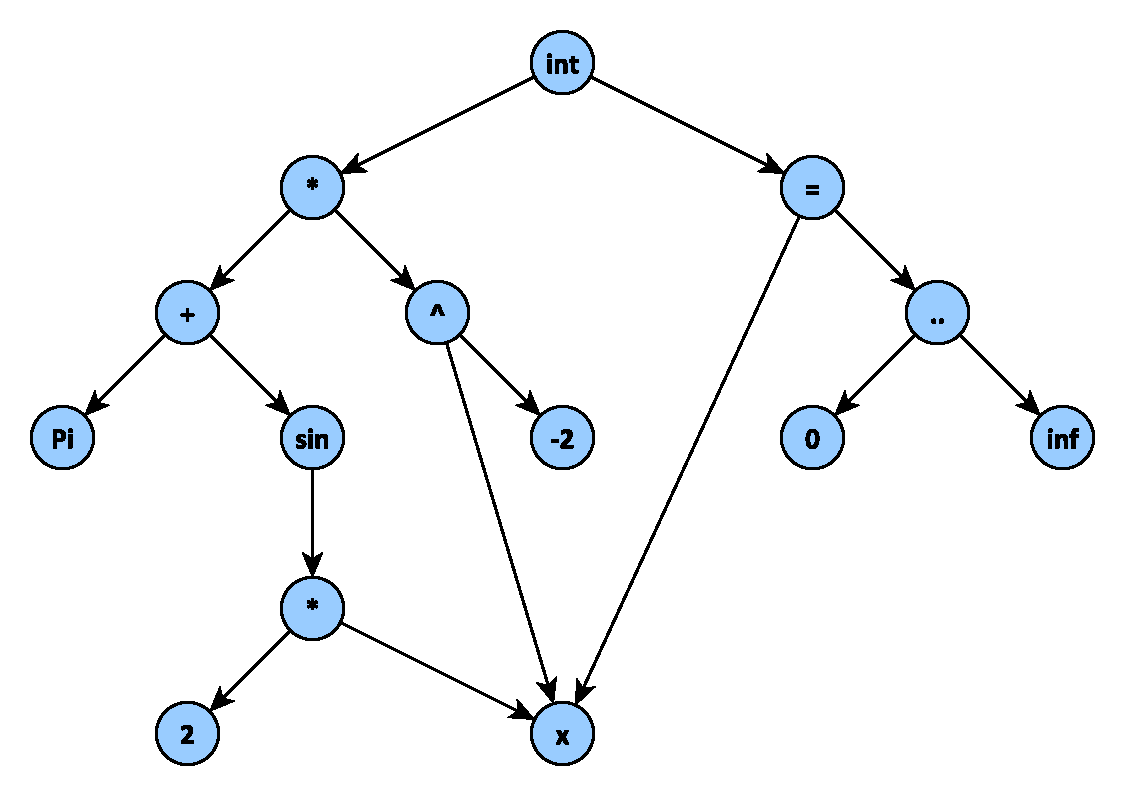
\includegraphics[scale=0.7]{DAG.pdf}
\caption{The \Maple{} DAG of equation~\eqref{eq:maple-input}}
\label{fig:maple-dag}
\end{figure}

The \Maple{} \gls{dag} can be visualized in a graph, such as in figure~\ref{fig:maple-dag}. But the internal representation looks a bit different. Each node in the \gls{dag} stores its children and has a header, which defines the type and the length of the node. Consider the polynomial $x^2+x$. Figure~\ref{fig:internal-maple-dag} illustrates the internal \gls{dag} representation with headers and arguments.

\begin{figure}[ht]
	\centering
	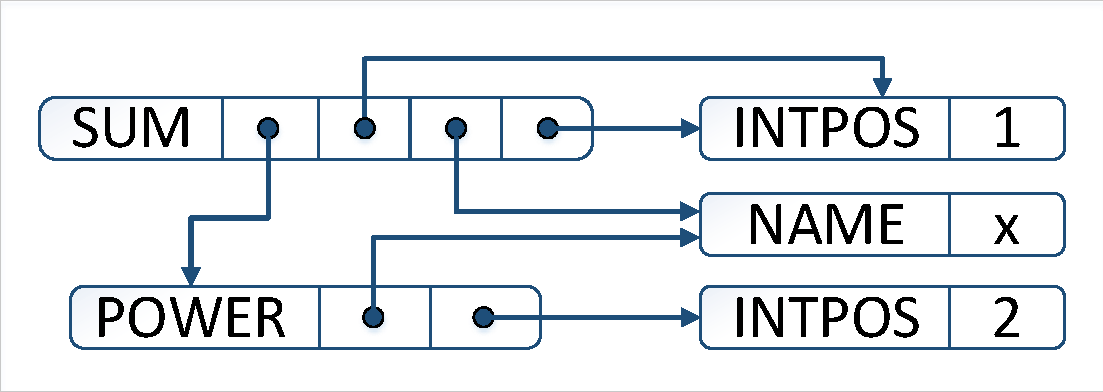
\includegraphics[clip, trim=0.1cm 0.1cm 0.1cm 0.1cm, scale=0.7]{DAGreal.pdf}
	\caption{The internal \Maple{} DAG representation of $x^2+x$.}
	\label{fig:internal-maple-dag}
\end{figure}

\Maple{} has also another representation, similar to the \gls{dag}, that allows multiple copies of the same object in its representation. This representation is called \inertF{} and is more similar to an expression tree than \Maple's \gls{dag}. The \inertF{} represents the \gls{dag} as a tree by splitting object copies and displays the tree in a list structure. Each node (or element in the list) has the prefix \texttt{\_Inert\_XXX}, that indicates the node is in the \inertF. The suffix \texttt{XXX} is the type of the node. Some of the important types are specified in table~\ref{tab:maple-types}. Note that this is only a subset of all possible types.

\begin{table}[ht]
\centering
\begin{tabular}{cp{10cm}}
	\hline
	Type & Explanation\\
	\hline
	SUM & Sums.\\
	PROD & Products.\\
	EXPSEQ & Expression sequence is a kind of list. The arguments of functions are stored in such sequences.\\
	INTPOS & Positive integers.\\
	INTNEG & Negative integers.\\
	COMPLEX & Complex numbers with real and imaginary part.\\
	FLOAT & Float numbers are stored in the scientific notation with integer values for the exponent $n$ and the significand $m$ in $m \cdot 10^n$.\\
	RATIONAL & Rational numbers are fractions stored in integer values for the numerator and positive integers for the denominator.\\
	POWER & Exponentiation with expressions as base and exponent.\\
	FUNCTION & Function invocation with the name, arguments and attributes of the function.\\
	\hline
\end{tabular}
\caption{A subset of important internal \Maple{} structures. See~\cite{MAPLE:ProgrammingGuide} for a complete list.}
\label{tab:maple-types}
\end{table}

\subsection{Maple's Open Maple API}
\Maple{} provides an \gls{api}, called \texttt{OpenMaple}~\cite[\S 14.3]{MAPLE:ProgrammingGuide} for interaction with the \Maple{} kernel. The \texttt{OpenMaple} \gls{api} is implemented for different programming languages such as \texttt{C}, \texttt{Java} and \texttt{Visual Basic}. Since our forward translation and the \gls{mlp} is implemented in \texttt{Java}, we use the \texttt{Java} \gls{api} for the backward translation. The \texttt{Java} \gls{api} has some limitations to interact with \Maple's \gls{dag}.

For the backward translation, we use the \inertF. This representation can be converted to a nested list version and the \texttt{OpenMaple} Java \gls{api} can handle lists. Therefore, the backward translation firstly converts the \inertF{} to a nested list structure before any translation process starts.

The following figure~\ref{fig:inertform-list} shows the \inertF{} and the nested list of the polynomial $x^2+x$.

\begin{figure}[ht]
\centering
\begin{minipage}{.45\linewidth}
\centering
\begin{tabular}{lll}
\multicolumn{3}{l}{\_Inert\_SUM(}\\
& \multicolumn{2}{l}{\_Inert\_POWER(}\\
& & \_Inert\_NAME("x"),\\
& & \_Inert\_INTPOS(2)\\
& ),\\ 
& \multicolumn{2}{l}{\_Inert\_NAME("x")}\\
)
\end{tabular}
\end{minipage}
\begin{minipage}{.45\linewidth}
\centering
\begin{tabular}{lll}
\multicolumn{3}{l}{[\_Inert\_SUM,}\\
& \multicolumn{2}{l}{[\_Inert\_POWER, }\\
& & [\_Inert\_NAME, "x"],\\
& & [\_Inert\_INTPOS, 2]\\
& ],\\ 
& \multicolumn{2}{l}{[\_Inert\_NAME, "x"]}\\
]
\end{tabular}
\end{minipage}
\caption{\inertF{} and the nested list representation of $x^2+x$.}
\label{fig:inertform-list}
\end{figure}

In the nested list, the first element specifies the type of the current list while the following arguments store the arguments and optional attributes.

\subsection{Workarounds for Problems}\label{subsec:maple-probs}
Note that the backward translations usually do not have problems with ambiguous expressions. Every \gls{cas} needs to solve ambiguities in its own representation, otherwise it could not compute the expression. Our backward translation from \Maple{} back to semantic \LaTeX{} is therefore based on already disambiguated expressions.

The general walkthrough of our backward translation starts with a string of a \texttt{1D} \Maple{} input expression. As described above, this string is entered in \Maple{} to parse the expression and work on the nested list version of the \inertF{} afterwards. This causes some problems. Mostly because \Maple{} automatically evaluates input expressions immediately - even before we have a chance to take a look at the internal data structure of the input. For example, an input such as $\sin@{\frac{\cpi}{2}}$ is immediately evaluated to $1$ and the internal data structure just shows us the positive integer value $1$ instead of the trigonometric function.

Furthermore, \Maple{} also changes input expressions slightly, mostly because of missing data types for a specific expression. For example, the internal data structure has no type to represent fractions except the \texttt{RATIONAL} type, which only allows integer values for the numerator and denominator. Thereby, an expression like $\frac{x}{2}$ is automatically changed to $x\frac{1}{2}$. There is no way no avoid such simple arithmetic changes in the expression, but we can avoid the automatic evaluations.

Firstly, we summarize all known changes and evaluations \Maple{} automatically performs on input expressions.

\begin{itemize}
\item \Maple{} evaluates input expressions immediately.
\item There is no data type to represents square roots such as $\sqrt{x}$ (or $n$-th roots). Therefore, \Maple{} stores roots as an exponentiation with a fractional exponent. For example, $\sqrt{x}$ is stored as $x^{\frac{1}{2}}$.
\item There is no data type for subtractions, only for sums. Negative terms are changed to absolute values times '$-1$'. For example, $x-y$ is stored as $x + y \cdot (-1)$. 
\item Floating point numbers are stored in the scientific notation with a mantissa and an exponent in the base $10$. For example, $3.1$ is internally represented as $31 \cdot 10^{-1}$.
\item There is only a data type for rational numbers (fractions with integer numerator and positive denominator), but not for general fractions, such as $\frac{x+y}{z}$. This will be automatically changed to $(x+y)\cdot z^{-1}$.
\end{itemize}

There are unevaluation quotes implemented to avoid evaluations on input expression. Table~\ref{tab:unevaluation-quotes} gives an example how those unevaluation quotes work.

\begin{table}[ht]
\centering
\begin{tabular}{lcc}
\hline
& Without unevaluation quotes & With unevalation quotes\\
\hline
Input expression: & \texttt{sin(Pi)+2-1} & \texttt{'sin(Pi)+2-1'}\\
Stored expression: & 1 & \texttt{sin(Pi)+1}\\
\hline
\end{tabular}
\caption{Example of unevaluation quotes for \texttt{1D} \Maple{} input expressions.}
\label{tab:unevaluation-quotes}
\end{table}

Since we want to keep a translated expression similar to the input expression, we use unevaluation quotes during the whole translation process. Unevaluation quotes also solve the problems with square roots and $n$-th roots. In \Maple's \texttt{1D} input representation, a square root is a function call (\texttt{sqrt(x)}) and the unevaluation quotes prevent evaluations on functions. Therefore, a backward translation simply needs to translate a square root as a normal function. Hence, we do not have problems with the internal representation of roots in \Maple.

Because of the absent data type for subtractions, a long sum with negative terms could be difficult to read. We change the order of constants (such as an integer value) to be in front of products. Therefore, an expression such as '$-y$' is not represented by '$y\cdot (-1)$', but by '$(-1) \cdot y$'. The translator now needs to check if there is a leading '$-1$' and can translate it to '$-y$' rather than to '$(-1) \cdot y$'.

Floating point numbers in scientific notation also causes a problem. Consider the input expression $0.41$ as the nested list \inertF{} representation
\begin{equation}
\texttt{[\_Inert\_FLOAT, [\_Inert\_INTPOS, 41], [\_Inert\_INTNEG, 2]]}.
\end{equation}

The backward translator is implemented in \texttt{Java}. To translate such an expression back to $0.41$, computations become necessary. Of course, it makes sense to perform those computations in the \gls{cas} (in that case, in \Maple) rather than in the translation program. Therefore, we implemented a procedure\footnote{\textit{Procedures} in \Maple{} are small programs similar to methods and functions in \gls{oop} languages.} to automatically convert \texttt{FLOAT} nodes to a string representation of the floating point number. We created a new type, called \texttt{MYFLOAT} to represent such numbers. With this approach, we avoided computations in the translation process.

For fractions, we use a similar approach and introduce a new internal data type \texttt{DIVIDE}. The implementation of \texttt{DIVIDE} was difficult. On the one hand, some expressions with negative exponent should be displayed as a fraction while others should should be displayed with the negative exponent. We follow the same rule as \Maple{} follows internally to display fractions. When the exponent is a negative numeric element, the expression should be displayed as a fraction. If the exponent is something else, we uses the negative exponent representation. Table~\ref{tab:maple-fracs} shows two examples with negative exponents. One of them is displayed as a fraction (exponent '$-2$') and the other is not (exponent '$-2y$'). We implement the same rule for our newly developed \texttt{DIVIDE} data type. Note that with the new created data type, we are still not able to avoid changes from $\frac{x}{2}$ to $x\frac{1}{2}$, but we are able to work with more general fraction expressions.

\begin{table}[ht]
\centering
\begin{tabular}{p{2.6cm}cc}
	\hline
	& Negative numeric exponent & General negative exponent\\
	\hline
	\texttt{1D} \Maple{} input expression & $\texttt{(x-1)\^{}(-2)}$ & \rule{0pt}{0.9\normalbaselineskip}$\texttt{(x-1)\^{}(-2*y)}$\\
	How \Maple{} displays the input & $\displaystyle\frac{1}{(x-1)^2}$ & $\displaystyle(x-1)^{-2y}$\\
	\hline
\end{tabular}
\caption{Different styles to display negative exponents depending on the type of the exponent. \Maple{} displays expressions with negative numeric exponents as fractions, while other negative exponents are not displayed as fractions.}
\label{tab:maple-fracs}
\end{table}

We implement all of these changes before the actual translation process starts. This helps keeping the translated expression similar to the input expression.

\subsection{Implementation Details}\label{subsec:maple-impl}
\begin{wrapfigure}{l}{0.485\textwidth}
	\vspace{-12pt}
	\centering
	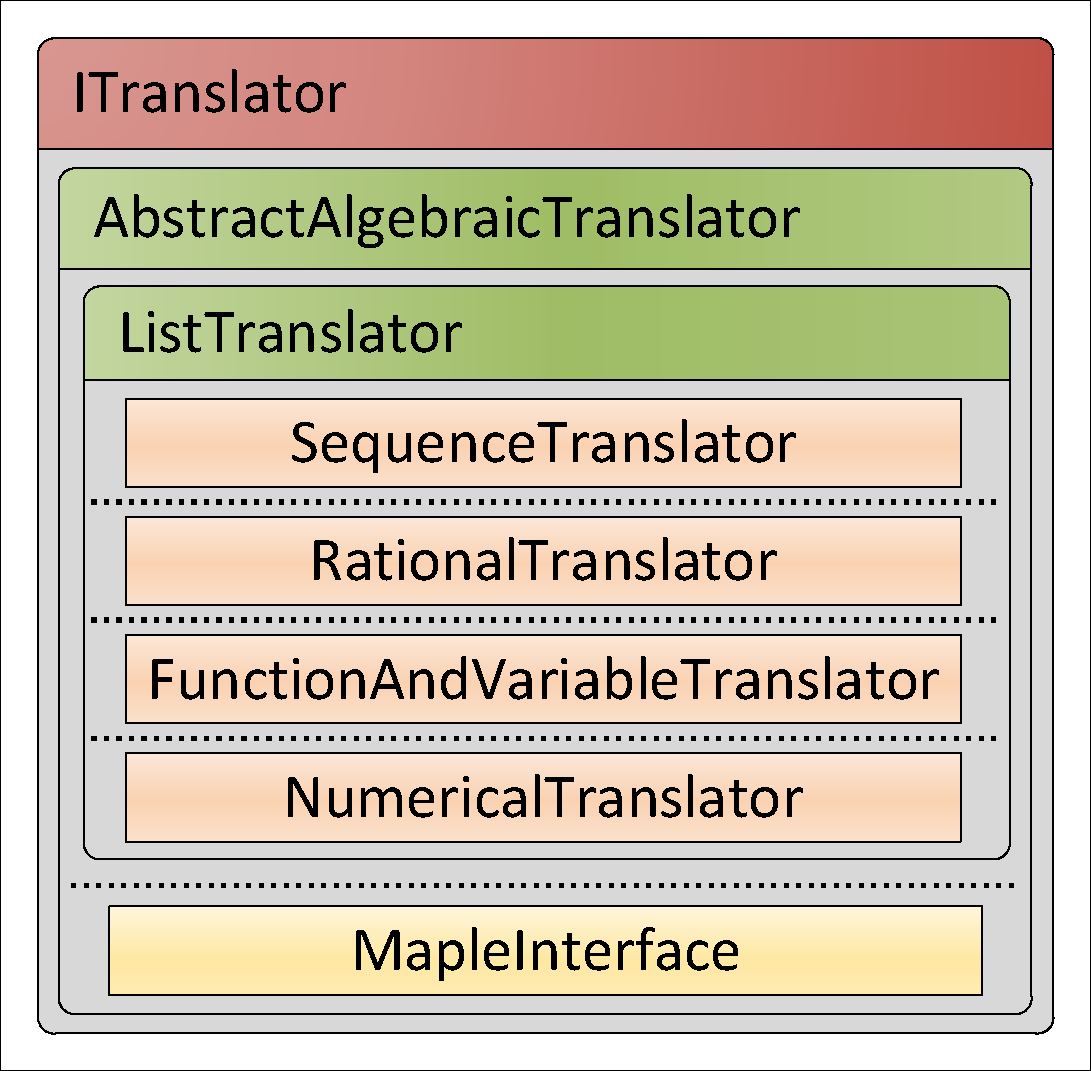
\includegraphics[clip, trim=0.1cm 0.1cm 0.1cm 0.1cm, scale=0.39]{BackwardTranslator.pdf}
	\caption{A scheme of the backward translator and its specialized subtranslators.}
	\label{fig:BackwardDel}
	\vspace{-13pt}
\end{wrapfigure}

The general translation process runs through different states. Each translation process starts with the string representation of a \texttt{1D} \Maple{} input. This string will be converted to the internal nested list representation of our custom \inertF{} (see the previous subsection~\ref{subsec:maple-probs}). Since the \inertF{} is similar to an expression tree, it can be translated as the \gls{mlp-pt} in the forward translation. Hence, we use the same approach of multiple subtranslators for the backward translation process.

Figure~\ref{fig:BackwardDel} shows the subtranslators of the backward translation process. The structure is the same as for the forward translation, seen in figure~\ref{fig:ForwardDel}. The \verb|MapleInterface| represents the entry point of a translation process. Before the translation starts, the \Maple{} kernel needs to be initialized and prepared for the translation process by loading all custom procedures. Once everything is loaded, an expression is delegated to specialized subtranslators depending on the internal data type, defined by custom procedures and \Maple's \inertF.

The following figure~\ref{fig:backward-trans} illustrates the backward translation process for the Jacobi polynomial example $\JacobiP{\alpha}{\beta}{n}@{\cos@{a\Theta}}$ from table~\ref{tab:JacobiP-usecase}. The input expression is converted to the nested list representation of the \texttt{MyInertForm} (the customized \inertF{} of \Maple). Afterwards, each node of the tree is translated separately by specialized subtranslators (visualized by blue arrows). The translation of functions (bold blue arrows) is again realized by translation patterns, which define the correct position for each argument. The last step is used to put all translated arguments to the right position (visualized by red arrows).

\begin{figure}[!htp]
	\centering
	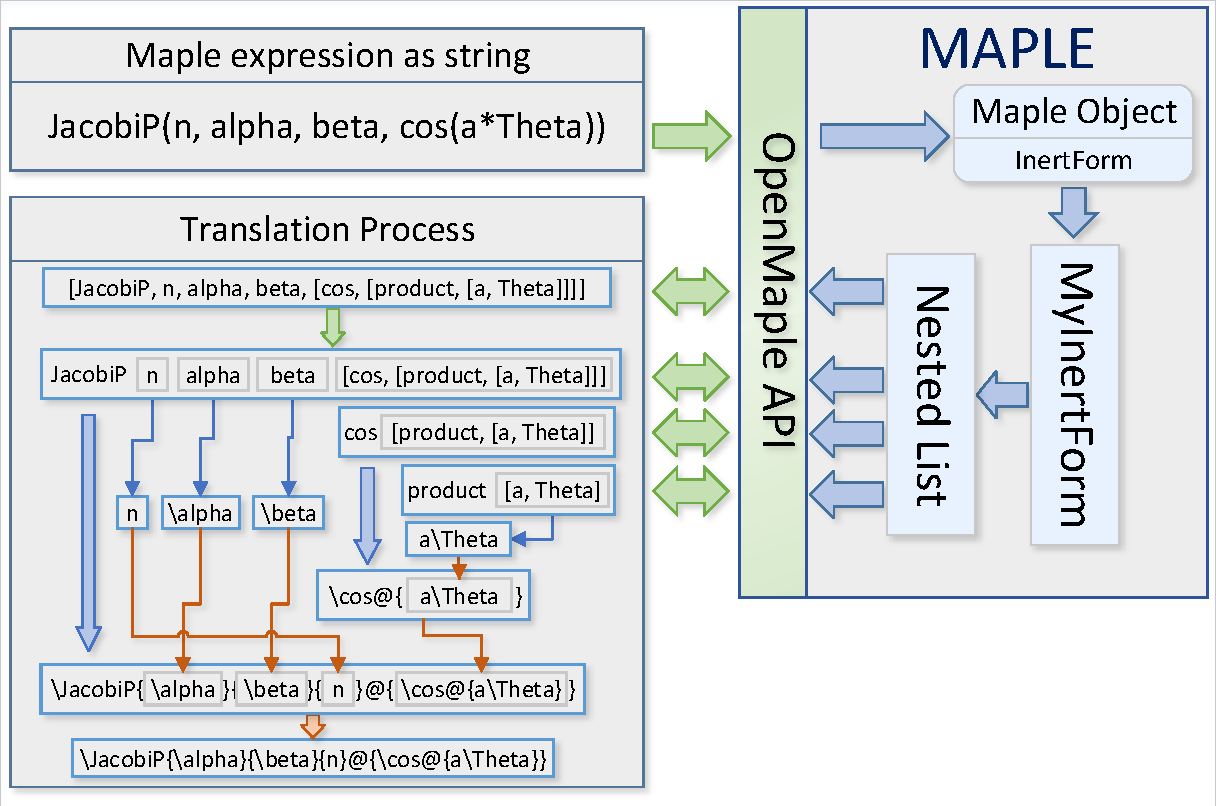
\includegraphics[clip, trim=0.1cm 0.1cm 0.1cm 0.1cm, scale=0.7]{MapleTranslation.pdf}
	\caption{A scheme of the backward translation process from \Maple{} for the Jacobi polynomial $\JacobiP{\alpha}{\beta}{n}@{\cos@{a\Theta}}$. The input string is converted by the \Maple{} kernel into the nested list representation. This list is translated by subtranslators (blue and red arrows). A function translation (bold blue arrows) is again realized by translation patterns to define the position of the arguments (red arrows).}
	\label{fig:backward-trans}
\end{figure}

\cleardoublepage

%\section{Evaluation}\label{ch:evaluation}
%\section{Evaluation}\label{sec:evaluation}
We implemented three approaches to evaluate whether a translation was \textit{appropriate} or \textit{inappropriate}.
\begin{enumerate}
\item \textbf{Round Trip Tests}: translates expressions back and forth and analyzing the changes.
\item \textbf{Function Relation Tests}: translate mathematically proven equivalent expressions from one system to a \gls*{cas} and evaluate whether the relation remains valid
\begin{enumerate}
\item via equivalence checks of the \gls*{cas} or
\item via numerical evaluation tests.
\end{enumerate}
\end{enumerate}

\subsection{Round Trip Tests}\label{sec:round-trip}
A round trip test always starts with a valid expression either in semantic \LaTeX{} or in \Maple. A translation from one system to another is called \textbf{a step}. A complete round trip translation (two steps) is called \textbf{one cycle}.

\begin{definition}[Fixed Point Representation]
A \textbf{fixed point representation} (or short fixed point) in a round trip translation process is a string representation that is identical to all string representations in the following cycles.
\end{definition}

Table~\ref{tab:fixpoint} illustrates an example of a round trip test which reaches a fixed point. The test formula is
\begin{equation}
\frac{\cos\left(a\Theta\right)}{2}.
\end{equation}

\begin{table}[ht]
\centering
\begin{tabular}{cc}
	\hline 
	Steps & semantic \LaTeX{}/\Maple{} representations\\
	\hline
	\rule{0pt}{0.9\normalbaselineskip}0 & \verb|\frac{\cos@{a\Theta}}{2}|\\
	1 & \verb|(cos(a*Theta))/(2)| \\
	2 & \verb|\frac{1}{2}\idot\cos@{a\idot\Theta}| \\
	3 & \verb|(1)/(2)*cos(a*Theta)|\\
	4 & \verb|\frac{1}{2}\idot\cos@{a\idot\Theta}| \\
	\hline
\end{tabular}
\caption{A round trip test reaching a fixed point.}
\label{tab:fixpoint}
\end{table}

Step 4 is identical to step 2, and since the translator is a deterministic algorithm it can be easily shown that step 2 and step 3 are fixed-point representations for semantic \LaTeX{} and \Maple.

There is currently only one exception known where a round trip test does not reach a fixed point representation: Legendre's incomplete elliptic integrals~\parencite[eq. 19.2.4-7]{NIST:DLMF} are defined with the amplitude $\phi$ in the first argument in the \DLMF, while \Maple{} takes the trigonometric sine of the amplitude as the first argument. Therefore, the forward and backward translations are defined as
\begin{eqnarray}
\verb|\EllIntF@{\phi}{k}| & \overset{\langMaple}{\mapsto} & \verb|EllipticF(sin(phi),k)|,\\
\verb|\EllIntF@{\asin@{\phi}}{k}| & \overset{\langMaple}{\mapsfrom} & \verb|EllipticF(phi,k)|,
\end{eqnarray}

And round-trip translations will produce infinite chains of sine and inverse sine calls. Since there are no evaluations involved, these chains will not be reduced during the translations. 
The round trip tests are very successful, but they only detect errors in string representations. However, because of the simplification techniques of fixed points, we are able to at least detect logical errors in one system: \Maple. On the other hand, these tests cannot determine logical errors in the translations between the two systems. Consider we mistakenly defined an \textit{inappropriate} forward and backward translation for the sine function
\begin{eqnarray}
\verb|\sin@{\phi}| & \overset{\langMaple}{\leftrightarrow} & \verb|cos(phi)|,\label{eq:wrong-trans-1}\\
\verb|\cos@{\phi}| & \overset{\langMaple}{\leftrightarrow} & \verb|sin(phi)|.\label{eq:wrong-trans-2}
\end{eqnarray}
In that case the round trip test would not detect any errors and reach a fixed point representation, because the simplification techniques only simplify two representations in the same system but cannot compare the representation in one system to those in the other.

\subsection{Function Relation Tests}\label{sec:relation-tests}
The \gls*{dlmf} is a compendium of special functions and orthogonal polynomials and lists several relations between the functions and polynomials. The idea of this evaluation approach is to translate an entire relation and test whether the relation remains valid after performing the translations.

With this technique we can detect translation errors such as in (\ref{eq:wrong-trans-1} and \ref{eq:wrong-trans-2}). Consider the \gls*{dlmf} equation for the sine and cosine function~\parencite[eq 4.21.2]{NIST:DLMF}
\begin{equation}
\sin \left(u+v\right) = \sin{u}\cos{v} + \cos{u}\sin{v}.
\end{equation}
Assume the translator would forward translate the expression based on (\ref{eq:wrong-trans-1},~\ref{eq:wrong-trans-2}). Than
\begin{eqnarray}
\verb|\sin@{u + v}| & \overset{\langMaple}{\mapsto} & \verb|cos(u + v)|,\\
\verb|\sin@@{u}\cos@@{v}| & \overset{\langMaple}{\mapsto} & \verb|cos(u)*sin(v)|,\\
\verb|\cos@@{u}\sin@@{v}| & \overset{\langMaple}{\mapsto} & \verb|sin(u)*cos(v)|.
\end{eqnarray}
This produces the equation in \Maple
\begin{equation}
\cos\left(u+v\right) = \cos{u}\sin{v} + \sin{u}\cos{v},
\end{equation}
which is wrong. Since the expression is correct before the translation, we conclude an error during the translation process.

However, there are two essential problems with this approach. Testing the mathematical equivalence of expressions is hard to solve and \gls*{cas} have trouble to test even simple equations. Furthermore, this approach only checks forward translations because there is no way to check equivalence of expressions in \LaTeX{} automatically (again this could become feasible with our translator). We use \Maple's \textit{simplify} function to check if the difference of the left-hand side and the right-hand side of the equation is equal to zero. In addition, we use \textit{simplify} and check if the division of the right-hand side by the left-hand side returns a numerical value or not. This simplification function is the most powerful function to check the equivalence in \Maple. However, there are several cases where the simplification fails. Because of implementation details, there are some techniques that helps \Maple{} to find possible simplifications. For example we can force \Maple{} to convert the formula
\begin{equation}
\sinh{x} + \sin{x}
\end{equation}
to an equivalent representation using the exponential representations
\begin{equation}
\frac{1}{2}\expe^x - \frac{1}{2}\expe^{-x} - \frac{1}{2} \iunit \left( \expe^{\iunit x}-\expe^{-\iunit x} \right).
\end{equation}
With such pre-conversions we are able to improve the simplification process in \Maple. However, the limitations of the \textit{simplify} function are still the weakest part of this verification approach. Consider the complex example~\parencite[eq. 12.7.10]{NIST:DLMF}
\begin{equation}\label{eq:branch-cut-near}
\displaystyle U(0,z) = \sqrt{\frac{z}{2\cpi}} K_{\frac{1}{4}}\left(\frac{1}{4}z^2\right),
\end{equation}
where $U(0,z)$ is the parabolic cylinder function and $K_\nu(z)$ the modified Bessel function of the second kind. Both functions are well-defined in both systems and we can define a \textit{direct} translation for~\eqref{eq:branch-cut-near}. 
The modified Bessel function of the second kind has its branch cut in \Maple{} and in the \gls*{dlmf} at $z < 0$. However, the argument of $K$ contains $z^2$. If $|\ph{z}| \in \left(\frac{\cpi}{2}, \cpi\right)$ the value of the right-hand side of~\eqref{eq:branch-cut-near} would be no longer on the principal branch. However, \Maple{} will still compute the principal values independently of the value of $z$. Hence, a translation
\begin{equation}
\verb|\BesselK{\frac{1}{4}}@{\frac{1}{4}z^2}| \overset{\langMaple}{\mapsto} \verb|BesselK(1/4,(1/4)*z^2)|
\end{equation}
is incorrect if $|\ph{z}| \in \left(\frac{\cpi}{2}, \cpi\right)$ and one has to use analytic continuation for the right-hand side of equation (\ref{eq:branch-cut-near}). 

To evaluate such complex cases, the equivalence checks of \gls*{cas} are insufficient. Therefore we implement numerical tests as an additional step.

\subsection{Numerical Tests}\label{sec:numerical-tests}
Consider the differences of the left- and right-hand side of equation~\eqref{eq:branch-cut-near}
\begin{equation}\label{eq:difference}
D(z) := U(0,z) - \sqrt{\frac{z}{2\cpi}} K_{\frac{1}{4}}\left(\frac{1}{4}z^2\right).
\end{equation}
Table~\ref{tab:computations-for-difference} presents four computations for $D(z)$, one value for each quadrant in the complex plane.
\begin{table}[ht]
\centering
\begin{tabular}{rcc}
	\hline
	$z\ \ $ & & $D(z)$\\
	\hline
	\tableRowSpace{} $1+\iunit$ & & $2 \cdot 10^{-10} - 2 \cdot 10^{-10} \iunit$\\
	$-1+\iunit$& & $2.222121916 - 1.116719816 \iunit$\\
	$-1-\iunit$& & $2.222121916 + 1.116719816 \iunit$\\
	$1-\iunit$ & & $2 \cdot 10^{-10} + 2 \cdot 10^{-10} \iunit$\\
	\hline
\end{tabular}
\caption{Four computations of $D(z)$ in \Maple.}
\label{tab:computations-for-difference}
\end{table}

Considering machine accuracy and the default precision of $10$ significant digits, we can regard the first and last values as zero differences. While this evaluation is very powerful, it has a significant problem. Even when all tested values return a value differ from zero, it does not proof the equivalence of~\eqref{eq:branch-cut-near}. However, when the values are different from zero, it does proof an error in one of the four cases~\parencite{NumericalTests:Paper}
\begin{enumerate}
\item the numerical engine tests invalid combinations of values;
\item the translation is incorrect;
\item there may be an error in the \gls*{dlmf} source; or
\item there may be an error in \Maple.
\end{enumerate}

\subsection{Results}\label{sec:test-summary}
There are 685 \Macro s\footnote{The macros are still work in progress, and therefore the total number is constantly changing.} in total, and 665 of them were implemented in the translator engine. We defined forward translations to \Maple{} for 201 and backward translations from \Maple{} for 195 functions. 

The \gls*{dlmf} provides a dataset of \LaTeX{} expressions with semantic macros. We extracted 4.087 equations from \gls*{dlmf} and apply our round-trip and relation tests on them. The translator was able to translate 2.405 (58.8\footnote{All percentages are approximately calculated.}\%) of the extracted equations without errors. 660 (27.4\%) of the successfully translated expressions were verified by the simplification techniques of \Maple. We apply additional numerical tests for the remaining 1.745 equations. For 418 (24\%) cases the numerical tests were valid. More detailed results for numerical and symbolical tests were presented in~\parencite{NumericalTests:Paper}.

The evaluation techniques have proven to be very powerful also for evaluating \gls*{cas} and online mathematical compendia such as the \gls*{dlmf}. During the evaluations, we were able to detect several errors in the translation and evaluation engine. However, even errors in the \gls*{dlmf} were discovered.

The numerical test engine was able to discover a sign error in equation~\parencite[eq. 14.5.14]{NIST:DLMF}\footnote{The equation had originally been stated as shown in equation~(\ref{eq:signerror}). The error were reported on 10th April 2017.}
\begin{equation}\label{eq:signerror}
\displaystyle \mathsf{Q}^{-1/2}_{\nu}\left(\cos\theta\right)=-\left(\frac{\pi}{2\sin\theta}\right)^{1/2}\frac{\cos\left(\left(\nu+\frac{1}{2}\right)\theta\right)}{\nu+\frac{1}{2}}.
\end{equation}
The error can be found on~\parencite[p. 359]{NIST:Handbook} and has been fixed in the \gls*{dlmf} with version 1.0.16. The same engine also identified a missing comma in the constraint of~\parencite[eq. 10.16.7]{NIST:DLMF}. The original constraint was given by $2\nu \neq -1, -2 -3, \ldots$, with a missing comma after $-2$.


%\section{Results \& Current Status}\label{ch:results}
%The goal is to develop an independent, lite translation tool between mathematical \LaTeX{} expressions and \gls{cas}. The semantic \LaTeX{} macros are constantly changing. Therefore, the translator can easily be updated as well, without implementing new code. Furthermore, we have implemented forward translations to the \gls{cas} \Maple{} and \Mathematica{} and a backward translation from \Maple. The translator is therefore able to allow complete round trip translations between \Maple{} and semantic \LaTeX. We have summarized the results of those validation techniques in chapter~\ref{ch:evaluation}.

The translator is based on not published code from the \gls{mlp} and \gls{pom}-tagger. Furthermore, the \Macro s are not published yet as well. Therefore, the current version of the translator is not online available yet. However, we are planning to publish the translator soon on the \gls{drmf} website\footnote{\url{http://drmf.wmflabs.org}}.

Our translator knows 665 \Macro s. We have defined forward translations for 201 of those to \Maple{} and 195 functions for backward translation from \Maple, plus translations for all Greek letters, constants and generic \LaTeX{} macros. The small percentage of covered macros is the translator's most important weakness. The reason is that most of the functions which are represented by a \Macro{} are not defined in \Maple. For example, the multivalued versions of the inverse trigonometric functions~\cite[(4.23.1-6)]{NIST:DLMF} and the $q$-generalizations are not defined in \Maple. A possible workaround is to define alternative translations based on the definition or other representations of the function, see the equations~\ref{eq:acot-alternatives} as an example. 

Nonetheless, the translator is able to handle a wide range of input expressions. This is shown by the test case of several formulae directly taken from the \DLMF. Out of 4165 test equations, 716 have been successfully forward translated to \Maple{} and proven to be correct by the internal simplification functions of \Maple. In addition, 1519 have been successfully forward translated to \Maple, but all validation methods failed. Thus, the translator is able to translate approximately $53.59\%$ of all test cases. Numerical test cases can advance the validation process and have been proven to be very powerful, but implementations of such automatic numerical tests are very complex and therefore not realized yet.
\newpage

\section{Bijection of Translations}
One of the main goals has been the provision of bijective mappings between semantic \LaTeX{} and \gls{cas}. This goal has not been achieved, because of the large number of functions that are only defined in one system, but not in the other. Our translations are in general neither injective nor surjective.

The forward translation is not injective, because there exist multiple macros for the same mathematical object. For example, the ultraspherical orthogonal polynomial (or Gegenbauer polynomial) has two macros and both are translated to the same function in the \gls{cas}. One of the macros is defined in the \gls{dlmf}, while the other is defined by the \gls{drmf}. For the background translation we choose the \gls{dlmf} representation.
\begin{eqnarray*}
	\verb|\Ultra{\lambda}{n}@{x}| & \overset{\langMaple}{\mapsto} & \verb|GegenbauerC(n, lambda, x)|,\\
	\verb|\Ultraspherical{\lambda}{n}@{x}| & \overset{\langMaple}{\mapsto} & \verb|GegenbauerC(n, lambda, x)|,\\
	\verb|\Ultraspherical{\lambda}{n}@{x}| & \overset{\langMaple}{\mapsfrom} & \verb|GegenbauerC(n, lambda, x)|.
\end{eqnarray*}

Deleting those multiple definitions from the set of macros would make a forward translation injective. Note that this is only true if two expressions are defined as identical as soon as their semantic meanings are identical. For example, formulae with a different number of white spaces are technically not identical, but will be translated to the same expression. However, those formulae can be defined as identical.

The forward translation is not surjective either, because obviously there are expressions in \gls{cas} which the translator would never produce. The same problems appear for the backward translation. For example, a backward translation from \Maple{} can never produce $\frac{x}{2}$, because of \Maple's internal changes it will only produce $x\frac{1}{2}$. Therefore, a backward translation is not surjective. Furthermore, it is not injective because of functions that cannot be translated yet.

However, for a subset of functions and expressions a bijective mapping is possible and has been proven by round trip tests. The main goal is therefore to enlarge these subsets. Mathematically, we looking for subsets $L_1 \subseteq \langTex$ and $L_2 \subseteq \langMaple$, such that $|L_1|$ and $|L_2|$ are maximal and $\mathrm{tr}^{L_1}_{L_2}$ is bijective and its inverse function is $\mathrm{tr}^{L_2}_{L_1}$.

\section{Supported CAS}
We support a forward translation to \Maple{} and \Mathematica. Nevertheless, the forward translation to \Mathematica{} is in an early state and only support a few translations for functions. Since the main work is already done for \Maple{}, one only needs to update the libraries for a better support of \Mathematica.

In theory it is possible to support even more \gls{cas}, but this has not been tested yet. Especially difficult are \gls{cas} that use different mathematical notations in their input format, such as the prefix notation. Those \gls{cas} cannot be supported as long as the \gls{mlp} does not produce expression trees. 

A backward translation has only been implemented for \Maple{} yet and it needs to have a licensed version of \Maple{} installed on the system to work, because access to the internal expression tree of \Maple{} expressions is necessary for the translator. Therefore, possible backward translations from other \gls{cas} also need access to the internal data structure.

\section{Open Problems}
One still unsolved problem are different branch cuts in two systems for the same mathematical function. Our workaround only provides additional information to the user, who needs to handle this issue on his own. However, we have presented an approach to solve this problem. Instead of translating the function itself, the translator could use equivalent formulae for the translation that only contain functions that use the same positions for branch cuts in both systems.

On the other hand, this approach does not solve the problem of the relation~(\ref{eq:branch-cut-near}), between the modified Bessel function of the second kind and the parabolic cylinder function. 
\begin{equation*}
\displaystyle \ParabolicU@{0}{z} = \sqrt{\frac{z}{2\cpi}}\BesselK{\frac{1}{4}}@{\frac{1}{4}z^2}
\end{equation*}
In this case, the problem is not an inconsistent definition of the position of the branch cuts, but that the variable $z$ jumps over branch cuts. While this is generally an issue of \gls{cas}, the translator could solve it automatically by using analytic continuation if necessary. This presumes that the translator can compute semantic \LaTeX{} expressions to detect critical values of $z^2$. Together with a \gls{cas}, this approach is feasible.

Another open problem are the verification techniques for translated expressions. While the backward translations are mostly verified by round trip tests, almost all of the translations need a powerful equivalence checker in the \gls{cas}. The limitations of this functionality are an important open problem for our validations. Furthermore, we currently need to assume the correctness of the used simplification functions. A bug in the simplification process spuriously verifying or mistakenly refusing the translation must be taken into consideration.

An approach to solve this problems are the described numerical tests. However, the verification of equivalence with a finite set of discrete values in a sufficient way, is an open problem.

Besides all of this, the translator still has problems with unclear semantics. One example are the already explained prime symbols to indicate derivatives. Another example are mathematical conventions for notations. For example, an expression
\begin{equation}
\sin^{-1}@{x}
\end{equation}
is mostly interpreted as the arcsine function $\asin@{x}$. However, our translator translates it as
\begin{equation}
\verb|\sin^{-1}@{x}| \overset{\langMaple}{\mapsto} \verb|1/(sin(x))|.
\end{equation}

Another problem are mismatched parenthesis. An expression for an half-opened interval $(a,b]$ currently returns an error because of the mismatch of the parenthesis. Nonetheless, this expression is valid for the representation of an interval.

We have also discovered a bug in the grammatical rules for the square root \LaTeX{} macro. The expression
\begin{equation}\label{eq:mlp-bug}
\verb|\sqrt \frac{a}{b}|
\end{equation}
produces an error. The generic \LaTeX{} macros always taken a fixed number of following expression as arguments. It is possible to group an expression with curly brackets. However, if there are no curly brackets used, a \LaTeX{} compiler interprets just one symbol as the argument. Therefore, the expression '\verb|\frac{a}{b}|' and '\verb|\frac ab|' produces the same output: $\frac ab$. The next symbol can also be a \LaTeX{} macro, such as in expression~(\ref{eq:mlp-bug}). Because the \gls{bnf} rule of the \gls{mlp} defines curly brackets currently as mandatory around the argument of the square root function, the \gls{mlp} produces an error during the parsing process.

%\section{Conclusion \& Future Work}\label{ch:conc-future-work}
%The results and conclusions of the translations of the formula set from the \DLMF{} are diverse. Some test cases have shown us that the set of semantic macros is not perfect yet and needs to be improved, seen in the example of the macro definition for the Wronskian symbol. However, simply adding more and more macros to improve the set is not the right decision. In that case we would end up in something similar to \sTeX, which is overloaded and too complicated to use. Obviously, if the system is no longer handy, it will not be used.

On the other hand, the concept of the translator has been proven. For example, one test case has revealed an overall sign error in an equation in the \DLMF~\cite[(14.5.14)]{NIST:DLMF} and therefore the validation system has shown the potential to become a strong verification tool for mathematical compendia. The test cases have also shown how difficult it is to validate a translated expression and have uncovered the problems of translations between two systems with different sets of supported functions. Our validation techniques also assume the correctness of the simplification and computational algorithms in \gls{cas}. However, combining those techniques and automatically running translation checks can potentially not only discover errors in mathematical compendia, but also detect errors in simplifications or computations in \gls{cas}.

Finally we can conclude that the project has been successful and the translator has great potential to become a handy translation tool. Nonetheless, it is without any doubts an ever-growing project and needs to be improved constantly.
%%\section{Approaches for Further Improvements}\label{sec:resolution}
As already discussed, the percentage of defined translations is small. Therefore, extending the backend libraries with additional translations for more semantic macros is the first obvious task to improve the translator. Adding more \gls{cas} would also be worthwhile for forward and backward translations. Some \gls{cas} or other software use other notations than the infix notations. Therefore, another improvement for the translator would be the support for other types of notations. This could be achieved by using expression trees during the translation process rather than the \gls{mlp-pt} generated by the \gls{mlp}.

Another minor issue is the way of representing functions after a backward translation. The \Macro s allow different representations and control the different styles by the number of $@$ symbols. Currently the backward translation simply adds the largest possible number of $@$ symbols, which has undesirable effects. Categorizing the functions (Possible categories may be \textit{trigonometric functions} or \textbf{polynomials}) can be used to define the right typical number of $@$ symbols for the most common representations.

Besides the extensions for the backend libraries, we saw in \cref{sec:numerical-tests} that automatic numerical tests are not implemented yet. Certainly, automatic numerical tests are a powerful approach to verify translations and also to find errors in the mathematical sources. However, the realization of such powerful numerical tests is very difficult. As far as we know, there is no general theory for such methods developed yet. An approach could be to adapt error handling methods in telecommunications such as the cyclic redundancy checks~\cite{CRC} that use checksums to detect errors. Adapting such approaches for general mathematical functions could be helpful.

The most desirable improvement for the translator is the support for generic \LaTeX. Since the semantic \LaTeX{} macros are newly invented and generic \LaTeX{} is still the de facto standard for mathematical expressions, it is definitely worthwhile to support generic \LaTeX{} later on. However, we already explained the difficulties of this task. One approach we want to realize is the \textbf{multiple-scan approach}. This approach is inspired by the approach of humans. When a human reader reads mathematical expressions, he concludes the correct semantics from the structure and the context of the expression. His conclusions highly depend on his own knowledge. If he is not familiar with a mathematical symbol, he has difficulties to understand the whole expression.

The multiple-scan approach tries to adapt these techniques with the following three objectives:
\begin{enumerate}[label=(\arabic*)]
\item\label{multi-scan-1} narrow down possible meanings only from the expression itself, without referring to the context of the expression;
\item\label{multi-scan-2} refine the process with conclusions from the nearby context of the expressions and
\item\label{multi-scan-3} improve the previous process by analyzing not only the nearby context but the overall topic of the whole scientific paper or book, its references and other publications by the authors.
\end{enumerate}
Starting with the lexicon files from the \gls{pom}-tagger, we want to narrow down the possible meanings of an expression. It is planned to extend the \gls{pom}-tagger from \cite{POM-Tagger} to achieve objective~\ref{multi-scan-1}. Furthermore, a large-scale corpus study has shown that around 70 percent of the symbolic elements in scientific papers are denoted in the surrounded text \cite{SymbolDec}. With this awareness we can achieve objective~\ref{multi-scan-2} by just searching the close context \cite{MLP:Project,SIGIR:Semantification,MORITZ:Evaluating}. If the correct semantic information is still unsure, objective~\ref{multi-scan-3} is the last way to find a solution. Online compendia, such as arXiv, can be used to discover the overall topic of a scientific paper, the references and the area of research of the authors. The MCAT search engine developed by Kristianto, Topic and Aizawa \cite{MCAT,MCAT:MathSemanticSearch} is able to extract and score information from the document at this '\textit{document granularity level}'. Ideally, there is only one possible interpretation left after step~\ref{multi-scan-3}. Otherwise, even a human reader might have difficulties to understand the expression.

Figure~\ref{fig:multiple-scan} visualizes the process of conclusions for the Jacobi polynomial example from \cref{tab:JacobiP-usecase}.

\begin{figure}[htp]
	\centering
	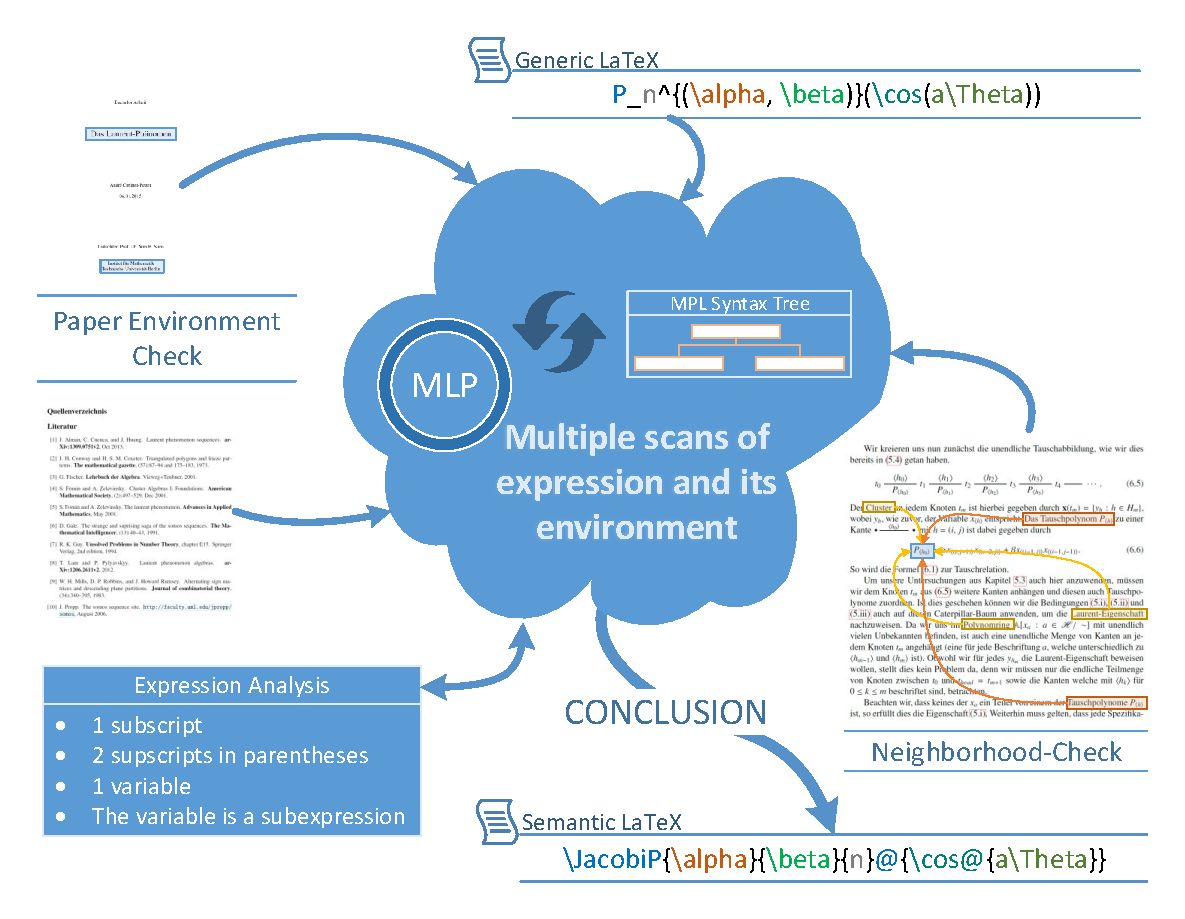
\includegraphics[clip, trim=0.1cm 0.1cm 0.1cm 0.1cm, scale=0.7]{MultipleScanApproach.pdf}
	\caption{Visualization of the multiple-scan approach. Exemplified using the Jacobi polynomial example.}
	\label{fig:multiple-scan}
\end{figure}

With such improvements the translator possibly becomes multifunctional: from automatic translations between word processors and computer algebra systems over to a verification tool for mathematical compendia, then over to a tool that can automatically enrich mathematical expressions with semantic information. A combination of the automatic semantically enrichment process and \LaTeX{} extraction tools~\cite{MaxTract} would be even hypothetically able to semantically enrich already published articles in PDF format afterwards.

\cleardoublepage

\emergencystretch=1em
%\phantomsection
%\addcontentsline{toc}{chapter}{Bibliography}
\printbibliography
\end{document}